% IEEE Access submission: single-file LaTeX source of the manuscript.
% Generated by scripts/17_ieee_access_bundle.py from paper/main_access_v2.tex; edit the
% repository sources, not this file. Compile: pdflatex main.tex (twice).
% SHORTENED IEEE Access version (v2). Same numbers, references and class as
% main_access.tex, with rewritten sections in sections_v2/ and new figures
% figs/v2_*.pdf (TikZ sources figs_src/v2_*_tikz.tex). main_access.tex is unchanged.
% generated numbers (generated/*.tex), figures and references as main.tex
% (neutral IEEEtran working format); only the front matter differs.
% Class files: access_template/ (provisional copy, see access_template/README.md;
% replace with the current official IEEE Access template before submission).
% Build: ./build.sh (compiles main.tex, main_access.tex and the supplement).
\documentclass{ieeeaccess}
\usepackage[T1]{fontenc}
\usepackage{amsmath,amssymb}
\usepackage{graphicx}
\usepackage{booktabs}
\usepackage{multirow}
\usepackage{makecell}
\usepackage{algorithm}
\usepackage{algpseudocode}
\usepackage{xcolor}
% TikZ does not work with this class; Fig. 1 is included as the PDF that build.sh
% renders from the same TikZ source (figs_src/pipeline_tikz.tex).
\def\UsePipelinePDF{}
\usepackage{url}
\usepackage{cite}
\usepackage[hidelinks]{hyperref}
\graphicspath{{./}}

% ---- begin generated/numbers.tex
% AUTO-GENERATED by scripts/05_make_tables.py -- do not edit
\newcommand{\AblAsymBayesCost}{0.825}
\newcommand{\AblAsymBayesPrAuc}{0.517}
\newcommand{\AblAsymBayesRecall}{79.8}
\newcommand{\AblAsymBayesRocAuc}{0.572}
\newcommand{\AblAsymBayesSpec}{32.0}
\newcommand{\AblAsymCostCost}{0.625}
\newcommand{\AblAsymCostPrAuc}{0.517}
\newcommand{\AblAsymCostRecall}{94.8}
\newcommand{\AblAsymCostRocAuc}{0.572}
\newcommand{\AblAsymCostSpec}{8.6}
\newcommand{\AblBalBayesCost}{0.890}
\newcommand{\AblBalBayesPrAuc}{0.486}
\newcommand{\AblBalBayesRecall}{76.6}
\newcommand{\AblBalBayesRocAuc}{0.554}
\newcommand{\AblBalBayesSpec}{33.1}
\newcommand{\AblBalCostCost}{0.660}
\newcommand{\AblBalCostPrAuc}{0.486}
\newcommand{\AblBalCostRecall}{94.3}
\newcommand{\AblBalCostRocAuc}{0.554}
\newcommand{\AblBalCostSpec}{4.3}
\newcommand{\AblDoubleBayesCost}{0.903}
\newcommand{\AblDoubleBayesPrAuc}{0.491}
\newcommand{\AblDoubleBayesRecall}{76.9}
\newcommand{\AblDoubleBayesRocAuc}{0.543}
\newcommand{\AblDoubleBayesSpec}{29.8}
\newcommand{\AblDoubleCostCost}{0.681}
\newcommand{\AblDoubleCostPrAuc}{0.491}
\newcommand{\AblDoubleCostRecall}{93.1}
\newcommand{\AblDoubleCostRocAuc}{0.543}
\newcommand{\AblDoubleCostSpec}{5.3}
\newcommand{\AblDuelBayesCost}{0.890}
\newcommand{\AblDuelBayesPrAuc}{0.494}
\newcommand{\AblDuelBayesRecall}{77.3}
\newcommand{\AblDuelBayesRocAuc}{0.559}
\newcommand{\AblDuelBayesSpec}{30.5}
\newcommand{\AblDuelCostCost}{0.644}
\newcommand{\AblDuelCostPrAuc}{0.494}
\newcommand{\AblDuelCostRecall}{94.6}
\newcommand{\AblDuelCostRocAuc}{0.559}
\newcommand{\AblDuelCostSpec}{5.8}
\newcommand{\AblFullBayesCost}{0.864}
\newcommand{\AblFullBayesPrAuc}{0.500}
\newcommand{\AblFullBayesRecall}{79.2}
\newcommand{\AblFullBayesRocAuc}{0.563}
\newcommand{\AblFullBayesSpec}{27.5}
\newcommand{\AblFullCostCost}{0.667}
\newcommand{\AblFullCostPrAuc}{0.500}
\newcommand{\AblFullCostRecall}{93.7}
\newcommand{\AblFullCostRocAuc}{0.563}
\newcommand{\AblFullCostSpec}{5.4}
\newcommand{\AblGammaZeroBayesCost}{0.825}
\newcommand{\AblGammaZeroBayesPrAuc}{0.510}
\newcommand{\AblGammaZeroBayesRecall}{80.6}
\newcommand{\AblGammaZeroBayesRocAuc}{0.576}
\newcommand{\AblGammaZeroBayesSpec}{29.2}
\newcommand{\AblGammaZeroCostCost}{0.645}
\newcommand{\AblGammaZeroCostPrAuc}{0.510}
\newcommand{\AblGammaZeroCostRecall}{94.4}
\newcommand{\AblGammaZeroCostRocAuc}{0.576}
\newcommand{\AblGammaZeroCostSpec}{6.4}
\newcommand{\AblSoftBayesCost}{0.804}
\newcommand{\AblSoftBayesPrAuc}{0.472}
\newcommand{\AblSoftBayesRecall}{82.9}
\newcommand{\AblSoftBayesRocAuc}{0.529}
\newcommand{\AblSoftBayesSpec}{23.5}
\newcommand{\AblSoftCostCost}{0.634}
\newcommand{\AblSoftCostPrAuc}{0.472}
\newcommand{\AblSoftCostRecall}{94.9}
\newcommand{\AblSoftCostRocAuc}{0.529}
\newcommand{\AblSoftCostSpec}{6.5}
\newcommand{\AblWarmBayesCost}{0.896}
\newcommand{\AblWarmBayesPrAuc}{0.497}
\newcommand{\AblWarmBayesRecall}{77.7}
\newcommand{\AblWarmBayesRocAuc}{0.547}
\newcommand{\AblWarmBayesSpec}{27.7}
\newcommand{\AblWarmCostCost}{0.656}
\newcommand{\AblWarmCostPrAuc}{0.497}
\newcommand{\AblWarmCostRecall}{93.8}
\newcommand{\AblWarmCostRocAuc}{0.547}
\newcommand{\AblWarmCostSpec}{7.1}
\newcommand{\AlwaysAcc}{44.2}
\newcommand{\AlwaysAlarm}{100.0}
\newcommand{\AlwaysBalAcc}{50.0}
\newcommand{\AlwaysCost}{0.558}
\newcommand{\AlwaysFN}{0}
\newcommand{\AlwaysFNR}{0.0}
\newcommand{\AlwaysFP}{5,243}
\newcommand{\AlwaysFPR}{100.0}
\newcommand{\AlwaysFone}{61.3}
\newcommand{\AlwaysGmean}{0.0}
\newcommand{\AlwaysMCC}{0.000}
\newcommand{\AlwaysPrec}{44.2}
\newcommand{\AlwaysRecall}{100.0}
\newcommand{\AlwaysSpec}{0.0}
\newcommand{\AlwaysTN}{0}
\newcommand{\AlwaysTP}{4,147}
\newcommand{\AttAucFracSmall}{87}
\newcommand{\AttAucMaxAbsChange}{0.089}
\newcommand{\AttAucNVariants}{17}
\newcommand{\AttEvasionDropMax}{19}
\newcommand{\AttEvasionDropMin}{4}
\newcommand{\BestBaseline}{RF}
\newcommand{\BestModelAUC}{HGB}
\newcommand{\BestModelCost}{RF}
\newcommand{\CSMLPAttAucMaxDrop}{0.025}
\newcommand{\CSMLPAttAucMaxRise}{0.005}
\newcommand{\CSMLPAttAucaccelspikes}{0.652}
\newcommand{\CSMLPAttAucclean}{0.654}
\newcommand{\CSMLPAttAucfpscap}{0.649}
\newcommand{\CSMLPAttAucrotjitter}{0.654}
\newcommand{\CSMLPAttAucrotsmooth}{0.646}
\newcommand{\CSMLPAttAucspeedscaledown}{0.629}
\newcommand{\CSMLPAttAucspeedscaleup}{0.630}
\newcommand{\CSMLPAttCleanFPR}{93.9}
\newcommand{\CSMLPAttCleanRecall}{99.4}
\newcommand{\CSMLPAttWorstFPR}{100.0}
\newcommand{\CSMLPAttWorstRecall}{95.6}
\newcommand{\CSMLPAttaccelspikesFPR}{99.1}
\newcommand{\CSMLPAttaccelspikesRecall}{99.9}
\newcommand{\CSMLPAttfpscapFPR}{98.3}
\newcommand{\CSMLPAttfpscapRecall}{100.0}
\newcommand{\CSMLPAttrotjitterFPR}{96.5}
\newcommand{\CSMLPAttrotjitterRecall}{99.7}
\newcommand{\CSMLPAttspeedscaleupFPR}{98.2}
\newcommand{\CSMLPAttspeedscaleupRecall}{100.0}
\newcommand{\CSMLPBayesAccEns}{57.4}
\newcommand{\CSMLPBayesAccMean}{57.0}
\newcommand{\CSMLPBayesAccSD}{1.5}
\newcommand{\CSMLPBayesAlarmEns}{73.5}
\newcommand{\CSMLPBayesAlarmMean}{72.1}
\newcommand{\CSMLPBayesAlarmSD}{2.2}
\newcommand{\CSMLPBayesBalAccEns}{60.3}
\newcommand{\CSMLPBayesBalAccMean}{59.7}
\newcommand{\CSMLPBayesBalAccSD}{1.6}
\newcommand{\CSMLPBayesCostEns}{0.691}
\newcommand{\CSMLPBayesCostMean}{0.731}
\newcommand{\CSMLPBayesCostSD}{0.066}
\newcommand{\CSMLPBayesFNEns}{622}
\newcommand{\CSMLPBayesFNMean}{707}
\newcommand{\CSMLPBayesFNREns}{15.0}
\newcommand{\CSMLPBayesFNRMean}{17.0}
\newcommand{\CSMLPBayesFNRSD}{3.1}
\newcommand{\CSMLPBayesFNSD}{129.7}
\newcommand{\CSMLPBayesFPEns}{3,381}
\newcommand{\CSMLPBayesFPMean}{3,332}
\newcommand{\CSMLPBayesFPREns}{64.5}
\newcommand{\CSMLPBayesFPRMean}{63.6}
\newcommand{\CSMLPBayesFPRSD}{2.3}
\newcommand{\CSMLPBayesFPSD}{118.2}
\newcommand{\CSMLPBayesFoneEns}{63.8}
\newcommand{\CSMLPBayesFoneMean}{63.0}
\newcommand{\CSMLPBayesFoneSD}{1.5}
\newcommand{\CSMLPBayesGmeanEns}{54.9}
\newcommand{\CSMLPBayesGmeanMean}{54.9}
\newcommand{\CSMLPBayesGmeanSD}{1.6}
\newcommand{\CSMLPBayesMCCEns}{0.231}
\newcommand{\CSMLPBayesMCCMean}{0.215}
\newcommand{\CSMLPBayesMCCSD}{0.037}
\newcommand{\CSMLPBayesPrAucEns}{0.529}
\newcommand{\CSMLPBayesPrAucMean}{0.521}
\newcommand{\CSMLPBayesPrAucSD}{0.022}
\newcommand{\CSMLPBayesPrecEns}{51.0}
\newcommand{\CSMLPBayesPrecMean}{50.8}
\newcommand{\CSMLPBayesPrecSD}{1.0}
\newcommand{\CSMLPBayesRecallEns}{85.0}
\newcommand{\CSMLPBayesRecallMean}{83.0}
\newcommand{\CSMLPBayesRecallSD}{3.1}
\newcommand{\CSMLPBayesRocAucEns}{0.654}
\newcommand{\CSMLPBayesRocAucMean}{0.644}
\newcommand{\CSMLPBayesRocAucSD}{0.018}
\newcommand{\CSMLPBayesSpecEns}{35.5}
\newcommand{\CSMLPBayesSpecMean}{36.4}
\newcommand{\CSMLPBayesSpecSD}{2.3}
\newcommand{\CSMLPBayesTNEns}{1,862}
\newcommand{\CSMLPBayesTNMean}{1,911}
\newcommand{\CSMLPBayesTNSD}{118.2}
\newcommand{\CSMLPBayesTPEns}{3,525}
\newcommand{\CSMLPBayesTPMean}{3,440}
\newcommand{\CSMLPBayesTPSD}{129.7}
\newcommand{\CSMLPCIBalAccHi}{55.1}
\newcommand{\CSMLPCIBalAccLo}{51.1}
\newcommand{\CSMLPCICostHi}{0.634}
\newcommand{\CSMLPCICostLo}{0.421}
\newcommand{\CSMLPCIMCCHi}{0.218}
\newcommand{\CSMLPCIMCCLo}{0.082}
\newcommand{\CSMLPCIPrAucHi}{0.712}
\newcommand{\CSMLPCIPrAucLo}{0.393}
\newcommand{\CSMLPCIRecallHi}{100.0}
\newcommand{\CSMLPCIRecallLo}{98.5}
\newcommand{\CSMLPCIRocAucHi}{0.781}
\newcommand{\CSMLPCIRocAucLo}{0.527}
\newcommand{\CSMLPCISpecHi}{10.8}
\newcommand{\CSMLPCISpecLo}{2.6}
\newcommand{\CSMLPCostAccEns}{47.3}
\newcommand{\CSMLPCostAccMean}{45.4}
\newcommand{\CSMLPCostAccSD}{0.9}
\newcommand{\CSMLPCostAlarmEns}{96.4}
\newcommand{\CSMLPCostAlarmMean}{98.1}
\newcommand{\CSMLPCostAlarmSD}{1.3}
\newcommand{\CSMLPCostBalAccEns}{52.8}
\newcommand{\CSMLPCostBalAccMean}{51.1}
\newcommand{\CSMLPCostBalAccSD}{0.8}
\newcommand{\CSMLPCostCostEns}{0.537}
\newcommand{\CSMLPCostCostMean}{0.557}
\newcommand{\CSMLPCostCostSD}{0.012}
\newcommand{\CSMLPCostFNEns}{23}
\newcommand{\CSMLPCostFNMean}{27}
\newcommand{\CSMLPCostFNREns}{0.6}
\newcommand{\CSMLPCostFNRMean}{0.6}
\newcommand{\CSMLPCostFNRSD}{0.7}
\newcommand{\CSMLPCostFNSD}{28.4}
\newcommand{\CSMLPCostFPEns}{4,925}
\newcommand{\CSMLPCostFPMean}{5,096}
\newcommand{\CSMLPCostFPREns}{93.9}
\newcommand{\CSMLPCostFPRMean}{97.2}
\newcommand{\CSMLPCostFPRSD}{1.9}
\newcommand{\CSMLPCostFPSD}{100.6}
\newcommand{\CSMLPCostFoneEns}{62.5}
\newcommand{\CSMLPCostFoneMean}{61.7}
\newcommand{\CSMLPCostFoneSD}{0.4}
\newcommand{\CSMLPCostGmeanEns}{24.6}
\newcommand{\CSMLPCostGmeanMean}{14.7}
\newcommand{\CSMLPCostGmeanSD}{8.8}
\newcommand{\CSMLPCostMCCEns}{0.146}
\newcommand{\CSMLPCostMCCMean}{0.072}
\newcommand{\CSMLPCostMCCSD}{0.049}
\newcommand{\CSMLPCostPrAucEns}{0.529}
\newcommand{\CSMLPCostPrAucMean}{0.521}
\newcommand{\CSMLPCostPrAucSD}{0.022}
\newcommand{\CSMLPCostPrecEns}{45.6}
\newcommand{\CSMLPCostPrecMean}{44.7}
\newcommand{\CSMLPCostPrecSD}{0.4}
\newcommand{\CSMLPCostRecallEns}{99.4}
\newcommand{\CSMLPCostRecallMean}{99.4}
\newcommand{\CSMLPCostRecallSD}{0.7}
\newcommand{\CSMLPCostRocAucEns}{0.654}
\newcommand{\CSMLPCostRocAucMean}{0.644}
\newcommand{\CSMLPCostRocAucSD}{0.018}
\newcommand{\CSMLPCostSpecEns}{6.1}
\newcommand{\CSMLPCostSpecMean}{2.8}
\newcommand{\CSMLPCostSpecSD}{1.9}
\newcommand{\CSMLPCostTNEns}{318}
\newcommand{\CSMLPCostTNMean}{147}
\newcommand{\CSMLPCostTNSD}{100.6}
\newcommand{\CSMLPCostTPEns}{4,124}
\newcommand{\CSMLPCostTPMean}{4,120}
\newcommand{\CSMLPCostTPSD}{28.4}
\newcommand{\CSMLPEvDelay}{0}
\newcommand{\CSMLPEvDetected}{26}
\newcommand{\CSMLPEvFreeAlarm}{88.1}
\newcommand{\CSMLPEvPreAlarm}{92.9}
\newcommand{\CSMLPMeanSeconds}{3}
\newcommand{\CSMLPMedBestEpoch}{14}
\newcommand{\CSMLPOptGap}{+0.033}
\newcommand{\CSMLPOptInner}{0.501}
\newcommand{\CSMLPQAbsMax}{nan}
\newcommand{\CSMLPRecAccEns}{51.4}
\newcommand{\CSMLPRecAccMean}{48.6}
\newcommand{\CSMLPRecAccSD}{2.1}
\newcommand{\CSMLPRecAlarmEns}{90.6}
\newcommand{\CSMLPRecAlarmMean}{94.0}
\newcommand{\CSMLPRecAlarmSD}{2.6}
\newcommand{\CSMLPRecBalAccEns}{56.2}
\newcommand{\CSMLPRecBalAccMean}{53.8}
\newcommand{\CSMLPRecBalAccSD}{1.9}
\newcommand{\CSMLPRecCostEns}{0.531}
\newcommand{\CSMLPRecCostMean}{0.544}
\newcommand{\CSMLPRecCostSD}{0.025}
\newcommand{\CSMLPRecFNEns}{105}
\newcommand{\CSMLPRecFNMean}{72}
\newcommand{\CSMLPRecFNREns}{2.5}
\newcommand{\CSMLPRecFNRMean}{1.7}
\newcommand{\CSMLPRecFNRSD}{1.2}
\newcommand{\CSMLPRecFNSD}{48.0}
\newcommand{\CSMLPRecFPEns}{4,463}
\newcommand{\CSMLPRecFPMean}{4,753}
\newcommand{\CSMLPRecFPREns}{85.1}
\newcommand{\CSMLPRecFPRMean}{90.7}
\newcommand{\CSMLPRecFPRSD}{4.2}
\newcommand{\CSMLPRecFPSD}{218.6}
\newcommand{\CSMLPRecFoneEns}{63.9}
\newcommand{\CSMLPRecFoneMean}{62.8}
\newcommand{\CSMLPRecFoneSD}{0.9}
\newcommand{\CSMLPRecGmeanEns}{38.1}
\newcommand{\CSMLPRecGmeanMean}{29.4}
\newcommand{\CSMLPRecGmeanSD}{8.0}
\newcommand{\CSMLPRecMCCEns}{0.210}
\newcommand{\CSMLPRecMCCMean}{0.156}
\newcommand{\CSMLPRecMCCSD}{0.052}
\newcommand{\CSMLPRecPrAucEns}{0.529}
\newcommand{\CSMLPRecPrAucMean}{0.521}
\newcommand{\CSMLPRecPrAucSD}{0.022}
\newcommand{\CSMLPRecPrecEns}{47.5}
\newcommand{\CSMLPRecPrecMean}{46.2}
\newcommand{\CSMLPRecPrecSD}{1.0}
\newcommand{\CSMLPRecRecallEns}{97.5}
\newcommand{\CSMLPRecRecallMean}{98.3}
\newcommand{\CSMLPRecRecallSD}{1.2}
\newcommand{\CSMLPRecRocAucEns}{0.654}
\newcommand{\CSMLPRecRocAucMean}{0.644}
\newcommand{\CSMLPRecRocAucSD}{0.018}
\newcommand{\CSMLPRecSpecEns}{14.9}
\newcommand{\CSMLPRecSpecMean}{9.3}
\newcommand{\CSMLPRecSpecSD}{4.2}
\newcommand{\CSMLPRecTNEns}{780}
\newcommand{\CSMLPRecTNMean}{490}
\newcommand{\CSMLPRecTNSD}{218.6}
\newcommand{\CSMLPRecTPEns}{4,042}
\newcommand{\CSMLPRecTPMean}{4,075}
\newcommand{\CSMLPRecTPSD}{48.0}
\newcommand{\CSMLPRocFPRatEightZero}{56.7}
\newcommand{\CSMLPRocFPRatNineFive}{84.4}
\newcommand{\CSMLPRocFPRatNineNine}{93.6}
\newcommand{\CSMLPRocFPRatNineZero}{75.9}
\newcommand{\CSMLPnProfile}{2}
\newcommand{\DOneFPRMax}{97}
\newcommand{\DOneFPRMin}{82}
\newcommand{\DQNAttAucMaxDrop}{0.064}
\newcommand{\DQNAttAucMaxRise}{0.035}
\newcommand{\DQNAttAucaccelspikes}{0.605}
\newcommand{\DQNAttAucclean}{0.665}
\newcommand{\DQNAttAucfpscap}{0.665}
\newcommand{\DQNAttAucrotjitter}{0.677}
\newcommand{\DQNAttAucrotsmooth}{0.676}
\newcommand{\DQNAttAucspeedscaledown}{0.632}
\newcommand{\DQNAttAucspeedscaleup}{0.680}
\newcommand{\DQNAttCleanFPR}{83.7}
\newcommand{\DQNAttCleanRecall}{96.9}
\newcommand{\DQNAttWorstFPR}{97.5}
\newcommand{\DQNAttWorstRecall}{87.3}
\newcommand{\DQNAttaccelspikesFPR}{95.4}
\newcommand{\DQNAttaccelspikesRecall}{97.9}
\newcommand{\DQNAttfpscapFPR}{83.7}
\newcommand{\DQNAttfpscapRecall}{96.9}
\newcommand{\DQNAttrotjitterFPR}{83.5}
\newcommand{\DQNAttrotjitterRecall}{94.8}
\newcommand{\DQNAttspeedscaleupFPR}{91.8}
\newcommand{\DQNAttspeedscaleupRecall}{97.8}
\newcommand{\DQNBayesAccEns}{58.6}
\newcommand{\DQNBayesAccMean}{58.3}
\newcommand{\DQNBayesAccSD}{1.0}
\newcommand{\DQNBayesAlarmEns}{73.7}
\newcommand{\DQNBayesAlarmMean}{72.7}
\newcommand{\DQNBayesAlarmSD}{1.2}
\newcommand{\DQNBayesBalAccEns}{61.5}
\newcommand{\DQNBayesBalAccMean}{61.1}
\newcommand{\DQNBayesBalAccSD}{1.0}
\newcommand{\DQNBayesCostEns}{0.653}
\newcommand{\DQNBayesCostMean}{0.680}
\newcommand{\DQNBayesCostSD}{0.035}
\newcommand{\DQNBayesFNEns}{561}
\newcommand{\DQNBayesFNMean}{617}
\newcommand{\DQNBayesFNREns}{13.5}
\newcommand{\DQNBayesFNRMean}{14.9}
\newcommand{\DQNBayesFNRSD}{1.7}
\newcommand{\DQNBayesFNSD}{68.5}
\newcommand{\DQNBayesFPEns}{3,330}
\newcommand{\DQNBayesFPMean}{3,297}
\newcommand{\DQNBayesFPREns}{63.5}
\newcommand{\DQNBayesFPRMean}{62.9}
\newcommand{\DQNBayesFPRSD}{1.5}
\newcommand{\DQNBayesFPSD}{78.6}
\newcommand{\DQNBayesFoneEns}{64.8}
\newcommand{\DQNBayesFoneMean}{64.3}
\newcommand{\DQNBayesFoneSD}{0.9}
\newcommand{\DQNBayesGmeanEns}{56.2}
\newcommand{\DQNBayesGmeanMean}{56.2}
\newcommand{\DQNBayesGmeanSD}{1.1}
\newcommand{\DQNBayesMCCEns}{0.259}
\newcommand{\DQNBayesMCCMean}{0.248}
\newcommand{\DQNBayesMCCSD}{0.022}
\newcommand{\DQNBayesPrAucEns}{0.606}
\newcommand{\DQNBayesPrAucMean}{0.595}
\newcommand{\DQNBayesPrAucSD}{0.022}
\newcommand{\DQNBayesPrecEns}{51.9}
\newcommand{\DQNBayesPrecMean}{51.7}
\newcommand{\DQNBayesPrecSD}{0.7}
\newcommand{\DQNBayesRecallEns}{86.5}
\newcommand{\DQNBayesRecallMean}{85.1}
\newcommand{\DQNBayesRecallSD}{1.7}
\newcommand{\DQNBayesRocAucEns}{0.665}
\newcommand{\DQNBayesRocAucMean}{0.661}
\newcommand{\DQNBayesRocAucSD}{0.013}
\newcommand{\DQNBayesSpecEns}{36.5}
\newcommand{\DQNBayesSpecMean}{37.1}
\newcommand{\DQNBayesSpecSD}{1.5}
\newcommand{\DQNBayesTNEns}{1,913}
\newcommand{\DQNBayesTNMean}{1,946}
\newcommand{\DQNBayesTNSD}{78.6}
\newcommand{\DQNBayesTPEns}{3,586}
\newcommand{\DQNBayesTPMean}{3,530}
\newcommand{\DQNBayesTPSD}{68.5}
\newcommand{\DQNCIBalAccHi}{61.1}
\newcommand{\DQNCIBalAccLo}{53.0}
\newcommand{\DQNCICostHi}{0.654}
\newcommand{\DQNCICostLo}{0.417}
\newcommand{\DQNCIMCCHi}{0.319}
\newcommand{\DQNCIMCCLo}{0.110}
\newcommand{\DQNCIPrAucHi}{0.778}
\newcommand{\DQNCIPrAucLo}{0.456}
\newcommand{\DQNCIRecallHi}{99.7}
\newcommand{\DQNCIRecallLo}{92.6}
\newcommand{\DQNCIRocAucHi}{0.785}
\newcommand{\DQNCIRocAucLo}{0.558}
\newcommand{\DQNCISpecHi}{24.8}
\newcommand{\DQNCISpecLo}{8.7}
\newcommand{\DQNCostAccEns}{51.9}
\newcommand{\DQNCostAccMean}{50.1}
\newcommand{\DQNCostAccSD}{1.9}
\newcommand{\DQNCostAlarmEns}{89.6}
\newcommand{\DQNCostAlarmMean}{89.8}
\newcommand{\DQNCostAlarmSD}{3.7}
\newcommand{\DQNCostBalAccEns}{56.6}
\newcommand{\DQNCostBalAccMean}{54.8}
\newcommand{\DQNCostBalAccSD}{1.6}
\newcommand{\DQNCostCostEns}{0.536}
\newcommand{\DQNCostCostMean}{0.584}
\newcommand{\DQNCostCostSD}{0.040}
\newcommand{\DQNCostFNEns}{129}
\newcommand{\DQNCostFNMean}{200}
\newcommand{\DQNCostFNREns}{3.1}
\newcommand{\DQNCostFNRMean}{4.8}
\newcommand{\DQNCostFNRSD}{2.7}
\newcommand{\DQNCostFNSD}{109.9}
\newcommand{\DQNCostFPEns}{4,391}
\newcommand{\DQNCostFPMean}{4,485}
\newcommand{\DQNCostFPREns}{83.7}
\newcommand{\DQNCostFPRMean}{85.5}
\newcommand{\DQNCostFPRSD}{4.9}
\newcommand{\DQNCostFPSD}{254.4}
\newcommand{\DQNCostFoneEns}{64.0}
\newcommand{\DQNCostFoneMean}{62.8}
\newcommand{\DQNCostFoneSD}{0.8}
\newcommand{\DQNCostGmeanEns}{39.7}
\newcommand{\DQNCostGmeanMean}{36.6}
\newcommand{\DQNCostGmeanSD}{5.8}
\newcommand{\DQNCostMCCEns}{0.213}
\newcommand{\DQNCostMCCMean}{0.158}
\newcommand{\DQNCostMCCSD}{0.038}
\newcommand{\DQNCostPrAucEns}{0.606}
\newcommand{\DQNCostPrAucMean}{0.595}
\newcommand{\DQNCostPrAucSD}{0.022}
\newcommand{\DQNCostPrecEns}{47.8}
\newcommand{\DQNCostPrecMean}{46.8}
\newcommand{\DQNCostPrecSD}{1.0}
\newcommand{\DQNCostRecallEns}{96.9}
\newcommand{\DQNCostRecallMean}{95.2}
\newcommand{\DQNCostRecallSD}{2.7}
\newcommand{\DQNCostRocAucEns}{0.665}
\newcommand{\DQNCostRocAucMean}{0.661}
\newcommand{\DQNCostRocAucSD}{0.013}
\newcommand{\DQNCostSpecEns}{16.3}
\newcommand{\DQNCostSpecMean}{14.5}
\newcommand{\DQNCostSpecSD}{4.9}
\newcommand{\DQNCostTNEns}{852}
\newcommand{\DQNCostTNMean}{758}
\newcommand{\DQNCostTNSD}{254.4}
\newcommand{\DQNCostTPEns}{4,018}
\newcommand{\DQNCostTPMean}{3,947}
\newcommand{\DQNCostTPSD}{109.9}
\newcommand{\DQNEvDelay}{0}
\newcommand{\DQNEvDetected}{25}
\newcommand{\DQNEvFreeAlarm}{70.4}
\newcommand{\DQNEvPreAlarm}{77.4}
\newcommand{\DQNGammas}{0, 0.9, 0.9, 0.9, 0}
\newcommand{\DQNMeanSeconds}{18}
\newcommand{\DQNMedBestEpoch}{8}
\newcommand{\DQNOptGap}{+0.065}
\newcommand{\DQNOptInner}{0.478}
\newcommand{\DQNOverest}{+0.393}
\newcommand{\DQNQAbsMax}{10.10}
\newcommand{\DQNRecAccEns}{55.8}
\newcommand{\DQNRecAccMean}{54.1}
\newcommand{\DQNRecAccSD}{1.3}
\newcommand{\DQNRecAlarmEns}{81.1}
\newcommand{\DQNRecAlarmMean}{84.3}
\newcommand{\DQNRecAlarmSD}{3.0}
\newcommand{\DQNRecBalAccEns}{59.5}
\newcommand{\DQNRecBalAccMean}{58.3}
\newcommand{\DQNRecBalAccSD}{1.2}
\newcommand{\DQNRecCostEns}{0.588}
\newcommand{\DQNRecCostMean}{0.573}
\newcommand{\DQNRecCostSD}{0.052}
\newcommand{\DQNRecFNEns}{343}
\newcommand{\DQNRecFNMean}{268}
\newcommand{\DQNRecFNREns}{8.3}
\newcommand{\DQNRecFNRMean}{6.5}
\newcommand{\DQNRecFNRSD}{2.9}
\newcommand{\DQNRecFNSD}{120.8}
\newcommand{\DQNRecFPEns}{3,810}
\newcommand{\DQNRecFPMean}{4,038}
\newcommand{\DQNRecFPREns}{72.7}
\newcommand{\DQNRecFPRMean}{77.0}
\newcommand{\DQNRecFPRSD}{3.4}
\newcommand{\DQNRecFPSD}{179.9}
\newcommand{\DQNRecFoneEns}{64.7}
\newcommand{\DQNRecFoneMean}{64.3}
\newcommand{\DQNRecFoneSD}{1.0}
\newcommand{\DQNRecGmeanEns}{50.1}
\newcommand{\DQNRecGmeanMean}{46.2}
\newcommand{\DQNRecGmeanSD}{3.0}
\newcommand{\DQNRecMCCEns}{0.242}
\newcommand{\DQNRecMCCMean}{0.227}
\newcommand{\DQNRecMCCSD}{0.032}
\newcommand{\DQNRecPrAucEns}{0.606}
\newcommand{\DQNRecPrAucMean}{0.595}
\newcommand{\DQNRecPrAucSD}{0.022}
\newcommand{\DQNRecPrecEns}{50.0}
\newcommand{\DQNRecPrecMean}{49.0}
\newcommand{\DQNRecPrecSD}{0.8}
\newcommand{\DQNRecRecallEns}{91.7}
\newcommand{\DQNRecRecallMean}{93.5}
\newcommand{\DQNRecRecallSD}{2.9}
\newcommand{\DQNRecRocAucEns}{0.665}
\newcommand{\DQNRecRocAucMean}{0.661}
\newcommand{\DQNRecRocAucSD}{0.013}
\newcommand{\DQNRecSpecEns}{27.3}
\newcommand{\DQNRecSpecMean}{23.0}
\newcommand{\DQNRecSpecSD}{3.4}
\newcommand{\DQNRecTNEns}{1,433}
\newcommand{\DQNRecTNMean}{1,205}
\newcommand{\DQNRecTNSD}{179.9}
\newcommand{\DQNRecTPEns}{3,804}
\newcommand{\DQNRecTPMean}{3,879}
\newcommand{\DQNRecTPSD}{120.8}
\newcommand{\DQNRocFPRatEightZero}{49.3}
\newcommand{\DQNRocFPRatNineFive}{82.4}
\newcommand{\DQNRocFPRatNineNine}{99.8}
\newcommand{\DQNRocFPRatNineZero}{76.5}
\newcommand{\DQNnProfile}{2}
\newcommand{\ECBAttAucMaxDrop}{0.089}
\newcommand{\ECBAttAucMaxRise}{0.052}
\newcommand{\ECBAttAucaccelspikes}{0.575}
\newcommand{\ECBAttAucclean}{0.659}
\newcommand{\ECBAttAucfpscap}{0.659}
\newcommand{\ECBAttAucrotjitter}{0.682}
\newcommand{\ECBAttAucrotsmooth}{0.658}
\newcommand{\ECBAttAucspeedscaledown}{0.648}
\newcommand{\ECBAttAucspeedscaleup}{0.648}
\newcommand{\ECBAttCleanFPR}{85.4}
\newcommand{\ECBAttCleanRecall}{96.6}
\newcommand{\ECBAttWorstFPR}{98.9}
\newcommand{\ECBAttWorstRecall}{78.0}
\newcommand{\ECBAttaccelspikesFPR}{97.7}
\newcommand{\ECBAttaccelspikesRecall}{99.3}
\newcommand{\ECBAttfpscapFPR}{85.4}
\newcommand{\ECBAttfpscapRecall}{96.6}
\newcommand{\ECBAttrotjitterFPR}{88.2}
\newcommand{\ECBAttrotjitterRecall}{96.1}
\newcommand{\ECBAttspeedscaleupFPR}{95.9}
\newcommand{\ECBAttspeedscaleupRecall}{98.7}
\newcommand{\ECBBayesAccEns}{58.6}
\newcommand{\ECBBayesAccMean}{58.7}
\newcommand{\ECBBayesAccSD}{1.6}
\newcommand{\ECBBayesAlarmEns}{72.2}
\newcommand{\ECBBayesAlarmMean}{73.0}
\newcommand{\ECBBayesAlarmSD}{2.3}
\newcommand{\ECBBayesBalAccEns}{61.3}
\newcommand{\ECBBayesBalAccMean}{61.5}
\newcommand{\ECBBayesBalAccSD}{1.5}
\newcommand{\ECBBayesCostEns}{0.681}
\newcommand{\ECBBayesCostMean}{0.663}
\newcommand{\ECBBayesCostSD}{0.044}
\newcommand{\ECBBayesFNEns}{627}
\newcommand{\ECBBayesFNMean}{587}
\newcommand{\ECBBayesFNREns}{15.1}
\newcommand{\ECBBayesFNRMean}{14.1}
\newcommand{\ECBBayesFNRSD}{2.2}
\newcommand{\ECBBayesFNSD}{90.3}
\newcommand{\ECBBayesFPEns}{3,262}
\newcommand{\ECBBayesFPMean}{3,291}
\newcommand{\ECBBayesFPREns}{62.2}
\newcommand{\ECBBayesFPRMean}{62.8}
\newcommand{\ECBBayesFPRSD}{3.0}
\newcommand{\ECBBayesFPSD}{159.4}
\newcommand{\ECBBayesFoneEns}{64.4}
\newcommand{\ECBBayesFoneMean}{64.7}
\newcommand{\ECBBayesFoneSD}{1.1}
\newcommand{\ECBBayesGmeanEns}{56.6}
\newcommand{\ECBBayesGmeanMean}{56.5}
\newcommand{\ECBBayesGmeanSD}{2.2}
\newcommand{\ECBBayesMCCEns}{0.251}
\newcommand{\ECBBayesMCCMean}{0.258}
\newcommand{\ECBBayesMCCSD}{0.031}
\newcommand{\ECBBayesPrAucEns}{0.565}
\newcommand{\ECBBayesPrAucMean}{0.562}
\newcommand{\ECBBayesPrAucSD}{0.006}
\newcommand{\ECBBayesPrecEns}{51.9}
\newcommand{\ECBBayesPrecMean}{52.0}
\newcommand{\ECBBayesPrecSD}{1.1}
\newcommand{\ECBBayesRecallEns}{84.9}
\newcommand{\ECBBayesRecallMean}{85.9}
\newcommand{\ECBBayesRecallSD}{2.2}
\newcommand{\ECBBayesRocAucEns}{0.659}
\newcommand{\ECBBayesRocAucMean}{0.653}
\newcommand{\ECBBayesRocAucSD}{0.011}
\newcommand{\ECBBayesSpecEns}{37.8}
\newcommand{\ECBBayesSpecMean}{37.2}
\newcommand{\ECBBayesSpecSD}{3.0}
\newcommand{\ECBBayesTNEns}{1,981}
\newcommand{\ECBBayesTNMean}{1,952}
\newcommand{\ECBBayesTNSD}{159.4}
\newcommand{\ECBBayesTPEns}{3,520}
\newcommand{\ECBBayesTPMean}{3,560}
\newcommand{\ECBBayesTPSD}{90.3}
\newcommand{\ECBCIBalAccHi}{59.6}
\newcommand{\ECBCIBalAccLo}{51.7}
\newcommand{\ECBCICostHi}{0.673}
\newcommand{\ECBCICostLo}{0.431}
\newcommand{\ECBCIMCCHi}{0.291}
\newcommand{\ECBCIMCCLo}{0.063}
\newcommand{\ECBCIPrAucHi}{0.740}
\newcommand{\ECBCIPrAucLo}{0.429}
\newcommand{\ECBCIRecallHi}{99.6}
\newcommand{\ECBCIRecallLo}{92.2}
\newcommand{\ECBCIRocAucHi}{0.767}
\newcommand{\ECBCIRocAucLo}{0.550}
\newcommand{\ECBCISpecHi}{21.4}
\newcommand{\ECBCISpecLo}{8.3}
\newcommand{\ECBCostAccEns}{50.8}
\newcommand{\ECBCostAccMean}{47.6}
\newcommand{\ECBCostAccSD}{1.2}
\newcommand{\ECBCostAlarmEns}{90.4}
\newcommand{\ECBCostAlarmMean}{94.0}
\newcommand{\ECBCostAlarmSD}{2.6}
\newcommand{\ECBCostBalAccEns}{55.6}
\newcommand{\ECBCostBalAccMean}{52.8}
\newcommand{\ECBCostBalAccSD}{1.2}
\newcommand{\ECBCostCostEns}{0.552}
\newcommand{\ECBCostCostMean}{0.575}
\newcommand{\ECBCostCostSD}{0.055}
\newcommand{\ECBCostFNEns}{140}
\newcommand{\ECBCostFNMean}{120}
\newcommand{\ECBCostFNREns}{3.4}
\newcommand{\ECBCostFNRMean}{2.9}
\newcommand{\ECBCostFNRSD}{2.9}
\newcommand{\ECBCostFNSD}{119.7}
\newcommand{\ECBCostFPEns}{4,480}
\newcommand{\ECBCostFPMean}{4,801}
\newcommand{\ECBCostFPREns}{85.4}
\newcommand{\ECBCostFPRMean}{91.6}
\newcommand{\ECBCostFPRSD}{2.8}
\newcommand{\ECBCostFPSD}{147.1}
\newcommand{\ECBCostFoneEns}{63.4}
\newcommand{\ECBCostFoneMean}{62.1}
\newcommand{\ECBCostFoneSD}{1.0}
\newcommand{\ECBCostGmeanEns}{37.5}
\newcommand{\ECBCostGmeanMean}{28.2}
\newcommand{\ECBCostGmeanSD}{5.0}
\newcommand{\ECBCostMCCEns}{0.188}
\newcommand{\ECBCostMCCMean}{0.122}
\newcommand{\ECBCostMCCSD}{0.052}
\newcommand{\ECBCostPrAucEns}{0.565}
\newcommand{\ECBCostPrAucMean}{0.562}
\newcommand{\ECBCostPrAucSD}{0.006}
\newcommand{\ECBCostPrecEns}{47.2}
\newcommand{\ECBCostPrecMean}{45.6}
\newcommand{\ECBCostPrecSD}{0.6}
\newcommand{\ECBCostRecallEns}{96.6}
\newcommand{\ECBCostRecallMean}{97.1}
\newcommand{\ECBCostRecallSD}{2.9}
\newcommand{\ECBCostRocAucEns}{0.659}
\newcommand{\ECBCostRocAucMean}{0.653}
\newcommand{\ECBCostRocAucSD}{0.011}
\newcommand{\ECBCostSpecEns}{14.6}
\newcommand{\ECBCostSpecMean}{8.4}
\newcommand{\ECBCostSpecSD}{2.8}
\newcommand{\ECBCostTNEns}{763}
\newcommand{\ECBCostTNMean}{442}
\newcommand{\ECBCostTNSD}{147.1}
\newcommand{\ECBCostTPEns}{4,007}
\newcommand{\ECBCostTPMean}{4,027}
\newcommand{\ECBCostTPSD}{119.7}
\newcommand{\ECBEvDelay}{0}
\newcommand{\ECBEvDetected}{25}
\newcommand{\ECBEvFreeAlarm}{76.9}
\newcommand{\ECBEvPreAlarm}{73.1}
\newcommand{\ECBMeanSeconds}{36}
\newcommand{\ECBMedBestEpoch}{8}
\newcommand{\ECBOptGap}{+0.070}
\newcommand{\ECBOptInner}{0.488}
\newcommand{\ECBOverest}{+0.088}
\newcommand{\ECBQAbsMax}{0.95}
\newcommand{\ECBRecAccEns}{53.0}
\newcommand{\ECBRecAccMean}{50.4}
\newcommand{\ECBRecAccSD}{1.5}
\newcommand{\ECBRecAlarmEns}{84.4}
\newcommand{\ECBRecAlarmMean}{89.5}
\newcommand{\ECBRecAlarmSD}{2.7}
\newcommand{\ECBRecBalAccEns}{57.1}
\newcommand{\ECBRecBalAccMean}{55.1}
\newcommand{\ECBRecBalAccSD}{1.4}
\newcommand{\ECBRecCostEns}{0.605}
\newcommand{\ECBRecCostMean}{0.581}
\newcommand{\ECBRecCostSD}{0.051}
\newcommand{\ECBRecFNEns}{317}
\newcommand{\ECBRecFNMean}{200}
\newcommand{\ECBRecFNREns}{7.6}
\newcommand{\ECBRecFNRMean}{4.8}
\newcommand{\ECBRecFNRSD}{2.7}
\newcommand{\ECBRecFNSD}{110.7}
\newcommand{\ECBRecFPEns}{4,093}
\newcommand{\ECBRecFPMean}{4,456}
\newcommand{\ECBRecFPREns}{78.1}
\newcommand{\ECBRecFPRMean}{85.0}
\newcommand{\ECBRecFPRSD}{3.3}
\newcommand{\ECBRecFPSD}{170.4}
\newcommand{\ECBRecFoneEns}{63.5}
\newcommand{\ECBRecFoneMean}{62.9}
\newcommand{\ECBRecFoneSD}{1.0}
\newcommand{\ECBRecGmeanEns}{45.0}
\newcommand{\ECBRecGmeanMean}{37.6}
\newcommand{\ECBRecGmeanSD}{4.2}
\newcommand{\ECBRecMCCEns}{0.195}
\newcommand{\ECBRecMCCMean}{0.167}
\newcommand{\ECBRecMCCSD}{0.042}
\newcommand{\ECBRecPrAucEns}{0.565}
\newcommand{\ECBRecPrAucMean}{0.562}
\newcommand{\ECBRecPrAucSD}{0.006}
\newcommand{\ECBRecPrecEns}{48.3}
\newcommand{\ECBRecPrecMean}{47.0}
\newcommand{\ECBRecPrecSD}{0.8}
\newcommand{\ECBRecRecallEns}{92.4}
\newcommand{\ECBRecRecallMean}{95.2}
\newcommand{\ECBRecRecallSD}{2.7}
\newcommand{\ECBRecRocAucEns}{0.659}
\newcommand{\ECBRecRocAucMean}{0.653}
\newcommand{\ECBRecRocAucSD}{0.011}
\newcommand{\ECBRecSpecEns}{21.9}
\newcommand{\ECBRecSpecMean}{15.0}
\newcommand{\ECBRecSpecSD}{3.3}
\newcommand{\ECBRecTNEns}{1,150}
\newcommand{\ECBRecTNMean}{787}
\newcommand{\ECBRecTNSD}{170.4}
\newcommand{\ECBRecTPEns}{3,830}
\newcommand{\ECBRecTPMean}{3,947}
\newcommand{\ECBRecTPSD}{110.7}
\newcommand{\ECBRocFPRatEightZero}{55.1}
\newcommand{\ECBRocFPRatNineFive}{84.5}
\newcommand{\ECBRocFPRatNineNine}{94.0}
\newcommand{\ECBRocFPRatNineZero}{69.4}
\newcommand{\ECBnProfile}{1}
\newcommand{\EDDQNAUCRank}{7}
\newcommand{\EDDQNAttAucMaxDrop}{0.008}
\newcommand{\EDDQNAttAucMaxRise}{0.053}
\newcommand{\EDDQNAttAucaccelspikes}{0.559}
\newcommand{\EDDQNAttAucclean}{0.541}
\newcommand{\EDDQNAttAucfpscap}{0.541}
\newcommand{\EDDQNAttAucrotjitter}{0.593}
\newcommand{\EDDQNAttAucrotsmooth}{0.539}
\newcommand{\EDDQNAttAucspeedscaledown}{0.532}
\newcommand{\EDDQNAttAucspeedscaleup}{0.561}
\newcommand{\EDDQNAttCleanFPR}{91.9}
\newcommand{\EDDQNAttCleanRecall}{90.4}
\newcommand{\EDDQNAttWorstFPR}{94.5}
\newcommand{\EDDQNAttWorstRecall}{82.9}
\newcommand{\EDDQNAttaccelspikesFPR}{94.3}
\newcommand{\EDDQNAttaccelspikesRecall}{95.4}
\newcommand{\EDDQNAttfpscapFPR}{91.9}
\newcommand{\EDDQNAttfpscapRecall}{90.4}
\newcommand{\EDDQNAttrotjitterFPR}{92.2}
\newcommand{\EDDQNAttrotjitterRecall}{94.0}
\newcommand{\EDDQNAttspeedscaleupFPR}{90.7}
\newcommand{\EDDQNAttspeedscaleupRecall}{93.5}
\newcommand{\EDDQNBayesAccEns}{49.2}
\newcommand{\EDDQNBayesAccMean}{49.8}
\newcommand{\EDDQNBayesAccSD}{2.5}
\newcommand{\EDDQNBayesAlarmEns}{75.6}
\newcommand{\EDDQNBayesAlarmMean}{74.3}
\newcommand{\EDDQNBayesAlarmSD}{1.3}
\newcommand{\EDDQNBayesBalAccEns}{52.2}
\newcommand{\EDDQNBayesBalAccMean}{52.6}
\newcommand{\EDDQNBayesBalAccSD}{2.7}
\newcommand{\EDDQNBayesCostEns}{0.895}
\newcommand{\EDDQNBayesCostMean}{0.905}
\newcommand{\EDDQNBayesCostSD}{0.092}
\newcommand{\EDDQNBayesFNEns}{909}
\newcommand{\EDDQNBayesFNMean}{944}
\newcommand{\EDDQNBayesFNREns}{21.9}
\newcommand{\EDDQNBayesFNRMean}{22.8}
\newcommand{\EDDQNBayesFNRSD}{3.8}
\newcommand{\EDDQNBayesFNSD}{159.0}
\newcommand{\EDDQNBayesFPEns}{3,862}
\newcommand{\EDDQNBayesFPMean}{3,774}
\newcommand{\EDDQNBayesFPREns}{73.7}
\newcommand{\EDDQNBayesFPRMean}{72.0}
\newcommand{\EDDQNBayesFPRSD}{2.0}
\newcommand{\EDDQNBayesFPSD}{104.1}
\newcommand{\EDDQNBayesFoneEns}{57.6}
\newcommand{\EDDQNBayesFoneMean}{57.6}
\newcommand{\EDDQNBayesFoneSD}{2.4}
\newcommand{\EDDQNBayesGmeanEns}{45.4}
\newcommand{\EDDQNBayesGmeanMean}{46.5}
\newcommand{\EDDQNBayesGmeanSD}{2.5}
\newcommand{\EDDQNBayesMCCEns}{0.051}
\newcommand{\EDDQNBayesMCCMean}{0.060}
\newcommand{\EDDQNBayesMCCSD}{0.061}
\newcommand{\EDDQNBayesPrAucEns}{0.496}
\newcommand{\EDDQNBayesPrAucMean}{0.483}
\newcommand{\EDDQNBayesPrAucSD}{0.019}
\newcommand{\EDDQNBayesPrecEns}{45.6}
\newcommand{\EDDQNBayesPrecMean}{45.9}
\newcommand{\EDDQNBayesPrecSD}{1.7}
\newcommand{\EDDQNBayesRecallEns}{78.1}
\newcommand{\EDDQNBayesRecallMean}{77.2}
\newcommand{\EDDQNBayesRecallSD}{3.8}
\newcommand{\EDDQNBayesRocAucEns}{0.541}
\newcommand{\EDDQNBayesRocAucMean}{0.538}
\newcommand{\EDDQNBayesRocAucSD}{0.016}
\newcommand{\EDDQNBayesSpecEns}{26.3}
\newcommand{\EDDQNBayesSpecMean}{28.0}
\newcommand{\EDDQNBayesSpecSD}{2.0}
\newcommand{\EDDQNBayesTNEns}{1,381}
\newcommand{\EDDQNBayesTNMean}{1,469}
\newcommand{\EDDQNBayesTNSD}{104.1}
\newcommand{\EDDQNBayesTPEns}{3,238}
\newcommand{\EDDQNBayesTPMean}{3,203}
\newcommand{\EDDQNBayesTPSD}{159.0}
\newcommand{\EDDQNCIBalAccHi}{54.9}
\newcommand{\EDDQNCIBalAccLo}{42.8}
\newcommand{\EDDQNCICostHi}{0.996}
\newcommand{\EDDQNCICostLo}{0.533}
\newcommand{\EDDQNCIMCCHi}{0.170}
\newcommand{\EDDQNCIMCCLo}{$-$0.229}
\newcommand{\EDDQNCIPrAucHi}{0.683}
\newcommand{\EDDQNCIPrAucLo}{0.329}
\newcommand{\EDDQNCIRecallHi}{98.9}
\newcommand{\EDDQNCIRecallLo}{77.7}
\newcommand{\EDDQNCIRocAucHi}{0.690}
\newcommand{\EDDQNCIRocAucLo}{0.382}
\newcommand{\EDDQNCISpecHi}{17.6}
\newcommand{\EDDQNCISpecLo}{1.5}
\newcommand{\EDDQNCostAccEns}{44.4}
\newcommand{\EDDQNCostAccMean}{45.4}
\newcommand{\EDDQNCostAccSD}{1.3}
\newcommand{\EDDQNCostAlarmEns}{91.2}
\newcommand{\EDDQNCostAlarmMean}{92.9}
\newcommand{\EDDQNCostAlarmSD}{2.3}
\newcommand{\EDDQNCostBalAccEns}{49.2}
\newcommand{\EDDQNCostBalAccMean}{50.4}
\newcommand{\EDDQNCostBalAccSD}{1.2}
\newcommand{\EDDQNCostCostEns}{0.726}
\newcommand{\EDDQNCostCostMean}{0.663}
\newcommand{\EDDQNCostCostSD}{0.048}
\newcommand{\EDDQNCostFNEns}{400}
\newcommand{\EDDQNCostFNMean}{274}
\newcommand{\EDDQNCostFNREns}{9.6}
\newcommand{\EDDQNCostFNRMean}{6.6}
\newcommand{\EDDQNCostFNRSD}{2.5}
\newcommand{\EDDQNCostFNSD}{102.8}
\newcommand{\EDDQNCostFPEns}{4,820}
\newcommand{\EDDQNCostFPMean}{4,854}
\newcommand{\EDDQNCostFPREns}{91.9}
\newcommand{\EDDQNCostFPRMean}{92.6}
\newcommand{\EDDQNCostFPRSD}{2.7}
\newcommand{\EDDQNCostFPSD}{139.9}
\newcommand{\EDDQNCostFoneEns}{58.9}
\newcommand{\EDDQNCostFoneMean}{60.2}
\newcommand{\EDDQNCostFoneSD}{0.9}
\newcommand{\EDDQNCostGmeanEns}{27.0}
\newcommand{\EDDQNCostGmeanMean}{26.0}
\newcommand{\EDDQNCostGmeanSD}{4.5}
\newcommand{\EDDQNCostMCCEns}{$-$0.028}
\newcommand{\EDDQNCostMCCMean}{0.016}
\newcommand{\EDDQNCostMCCSD}{0.054}
\newcommand{\EDDQNCostPrAucEns}{0.496}
\newcommand{\EDDQNCostPrAucMean}{0.483}
\newcommand{\EDDQNCostPrAucSD}{0.019}
\newcommand{\EDDQNCostPrecEns}{43.7}
\newcommand{\EDDQNCostPrecMean}{44.4}
\newcommand{\EDDQNCostPrecSD}{0.7}
\newcommand{\EDDQNCostRank}{7}
\newcommand{\EDDQNCostRecallEns}{90.4}
\newcommand{\EDDQNCostRecallMean}{93.4}
\newcommand{\EDDQNCostRecallSD}{2.5}
\newcommand{\EDDQNCostRocAucEns}{0.541}
\newcommand{\EDDQNCostRocAucMean}{0.538}
\newcommand{\EDDQNCostRocAucSD}{0.016}
\newcommand{\EDDQNCostSpecEns}{8.1}
\newcommand{\EDDQNCostSpecMean}{7.4}
\newcommand{\EDDQNCostSpecSD}{2.7}
\newcommand{\EDDQNCostTNEns}{423}
\newcommand{\EDDQNCostTNMean}{389}
\newcommand{\EDDQNCostTNSD}{139.9}
\newcommand{\EDDQNCostTPEns}{3,747}
\newcommand{\EDDQNCostTPMean}{3,873}
\newcommand{\EDDQNCostTPSD}{102.8}
\newcommand{\EDDQNEvDelay}{0}
\newcommand{\EDDQNEvDetected}{26}
\newcommand{\EDDQNEvFreeAlarm}{96.6}
\newcommand{\EDDQNEvPreAlarm}{82.3}
\newcommand{\EDDQNFeatureSets}{exposure+profile, exposure+profile, exposure+profile, exposure+profile, exposure+profile}
\newcommand{\EDDQNGammas}{0.99, 0.99, 0.99, 0.99, 0.9}
\newcommand{\EDDQNMeanSeconds}{19}
\newcommand{\EDDQNMedBestEpoch}{8}
\newcommand{\EDDQNOptGap}{+0.288}
\newcommand{\EDDQNOptInner}{0.467}
\newcommand{\EDDQNOverest}{$-$2.900}
\newcommand{\EDDQNQAbsMax}{61.78}
\newcommand{\EDDQNRecAccEns}{44.8}
\newcommand{\EDDQNRecAccMean}{44.7}
\newcommand{\EDDQNRecAccSD}{1.7}
\newcommand{\EDDQNRecAlarmEns}{85.7}
\newcommand{\EDDQNRecAlarmMean}{87.8}
\newcommand{\EDDQNRecAlarmSD}{2.8}
\newcommand{\EDDQNRecBalAccEns}{49.0}
\newcommand{\EDDQNRecBalAccMean}{49.1}
\newcommand{\EDDQNRecBalAccSD}{1.7}
\newcommand{\EDDQNRecCostEns}{0.825}
\newcommand{\EDDQNRecCostMean}{0.785}
\newcommand{\EDDQNRecCostSD}{0.062}
\newcommand{\EDDQNRecFNEns}{641}
\newcommand{\EDDQNRecFNMean}{546}
\newcommand{\EDDQNRecFNREns}{15.5}
\newcommand{\EDDQNRecFNRMean}{13.2}
\newcommand{\EDDQNRecFNRSD}{3.1}
\newcommand{\EDDQNRecFNSD}{128.7}
\newcommand{\EDDQNRecFPEns}{4,539}
\newcommand{\EDDQNRecFPMean}{4,642}
\newcommand{\EDDQNRecFPREns}{86.6}
\newcommand{\EDDQNRecFPRMean}{88.5}
\newcommand{\EDDQNRecFPRSD}{3.4}
\newcommand{\EDDQNRecFPSD}{176.0}
\newcommand{\EDDQNRecFoneEns}{57.5}
\newcommand{\EDDQNRecFoneMean}{58.1}
\newcommand{\EDDQNRecFoneSD}{1.3}
\newcommand{\EDDQNRecGmeanEns}{33.7}
\newcommand{\EDDQNRecGmeanMean}{31.2}
\newcommand{\EDDQNRecGmeanSD}{4.3}
\newcommand{\EDDQNRecMCCEns}{$-$0.029}
\newcommand{\EDDQNRecMCCMean}{$-$0.027}
\newcommand{\EDDQNRecMCCSD}{0.053}
\newcommand{\EDDQNRecPrAucEns}{0.496}
\newcommand{\EDDQNRecPrAucMean}{0.483}
\newcommand{\EDDQNRecPrAucSD}{0.019}
\newcommand{\EDDQNRecPrecEns}{43.6}
\newcommand{\EDDQNRecPrecMean}{43.7}
\newcommand{\EDDQNRecPrecSD}{0.9}
\newcommand{\EDDQNRecRecallEns}{84.5}
\newcommand{\EDDQNRecRecallMean}{86.8}
\newcommand{\EDDQNRecRecallSD}{3.1}
\newcommand{\EDDQNRecRocAucEns}{0.541}
\newcommand{\EDDQNRecRocAucMean}{0.538}
\newcommand{\EDDQNRecRocAucSD}{0.016}
\newcommand{\EDDQNRecSpecEns}{13.4}
\newcommand{\EDDQNRecSpecMean}{11.5}
\newcommand{\EDDQNRecSpecSD}{3.4}
\newcommand{\EDDQNRecTNEns}{704}
\newcommand{\EDDQNRecTNMean}{601}
\newcommand{\EDDQNRecTNSD}{176.0}
\newcommand{\EDDQNRecTPEns}{3,506}
\newcommand{\EDDQNRecTPMean}{3,601}
\newcommand{\EDDQNRecTPSD}{128.7}
\newcommand{\EDDQNRocFPRatEightZero}{75.3}
\newcommand{\EDDQNRocFPRatNineFive}{97.7}
\newcommand{\EDDQNRocFPRatNineNine}{99.6}
\newcommand{\EDDQNRocFPRatNineZero}{91.8}
\newcommand{\EDDQNnFullInfo}{3}
\newcommand{\EDDQNnGammaZero}{0}
\newcommand{\EDDQNnProfile}{5}
\newcommand{\HGBAttAucMaxDrop}{0.068}
\newcommand{\HGBAttAucMaxRise}{0.019}
\newcommand{\HGBAttAucaccelspikes}{0.698}
\newcommand{\HGBAttAucclean}{0.692}
\newcommand{\HGBAttAucfpscap}{0.694}
\newcommand{\HGBAttAucrotjitter}{0.709}
\newcommand{\HGBAttAucrotsmooth}{0.712}
\newcommand{\HGBAttAucspeedscaledown}{0.647}
\newcommand{\HGBAttAucspeedscaleup}{0.650}
\newcommand{\HGBAttCleanFPR}{85.4}
\newcommand{\HGBAttCleanRecall}{97.0}
\newcommand{\HGBAttWorstFPR}{96.1}
\newcommand{\HGBAttWorstRecall}{81.0}
\newcommand{\HGBAttaccelspikesFPR}{95.7}
\newcommand{\HGBAttaccelspikesRecall}{98.1}
\newcommand{\HGBAttfpscapFPR}{85.9}
\newcommand{\HGBAttfpscapRecall}{97.0}
\newcommand{\HGBAttrotjitterFPR}{82.7}
\newcommand{\HGBAttrotjitterRecall}{96.3}
\newcommand{\HGBAttspeedscaleupFPR}{91.7}
\newcommand{\HGBAttspeedscaleupRecall}{98.2}
\newcommand{\HGBBayesAccEns}{57.4}
\newcommand{\HGBBayesAccMean}{57.4}
\newcommand{\HGBBayesAccSD}{0.0}
\newcommand{\HGBBayesAlarmEns}{79.7}
\newcommand{\HGBBayesAlarmMean}{79.7}
\newcommand{\HGBBayesAlarmSD}{0.0}
\newcommand{\HGBBayesBalAccEns}{61.0}
\newcommand{\HGBBayesBalAccMean}{61.0}
\newcommand{\HGBBayesBalAccSD}{0.0}
\newcommand{\HGBBayesCostEns}{0.567}
\newcommand{\HGBBayesCostMean}{0.567}
\newcommand{\HGBBayesCostSD}{0.000}
\newcommand{\HGBBayesFNEns}{331}
\newcommand{\HGBBayesFNMean}{331}
\newcommand{\HGBBayesFNREns}{8.0}
\newcommand{\HGBBayesFNRMean}{8.0}
\newcommand{\HGBBayesFNRSD}{0.0}
\newcommand{\HGBBayesFNSD}{0.0}
\newcommand{\HGBBayesFPEns}{3,670}
\newcommand{\HGBBayesFPMean}{3,670}
\newcommand{\HGBBayesFPREns}{70.0}
\newcommand{\HGBBayesFPRMean}{70.0}
\newcommand{\HGBBayesFPRSD}{0.0}
\newcommand{\HGBBayesFPSD}{0.0}
\newcommand{\HGBBayesFoneEns}{65.6}
\newcommand{\HGBBayesFoneMean}{65.6}
\newcommand{\HGBBayesFoneSD}{0.0}
\newcommand{\HGBBayesGmeanEns}{52.5}
\newcommand{\HGBBayesGmeanMean}{52.5}
\newcommand{\HGBBayesGmeanSD}{0.0}
\newcommand{\HGBBayesMCCEns}{0.272}
\newcommand{\HGBBayesMCCMean}{0.272}
\newcommand{\HGBBayesMCCSD}{0.000}
\newcommand{\HGBBayesPrAucEns}{0.593}
\newcommand{\HGBBayesPrAucMean}{0.593}
\newcommand{\HGBBayesPrAucSD}{0.000}
\newcommand{\HGBBayesPrecEns}{51.0}
\newcommand{\HGBBayesPrecMean}{51.0}
\newcommand{\HGBBayesPrecSD}{0.0}
\newcommand{\HGBBayesRecallEns}{92.0}
\newcommand{\HGBBayesRecallMean}{92.0}
\newcommand{\HGBBayesRecallSD}{0.0}
\newcommand{\HGBBayesRocAucEns}{0.692}
\newcommand{\HGBBayesRocAucMean}{0.692}
\newcommand{\HGBBayesRocAucSD}{0.000}
\newcommand{\HGBBayesSpecEns}{30.0}
\newcommand{\HGBBayesSpecMean}{30.0}
\newcommand{\HGBBayesSpecSD}{0.0}
\newcommand{\HGBBayesTNEns}{1,573}
\newcommand{\HGBBayesTNMean}{1,573}
\newcommand{\HGBBayesTNSD}{0.0}
\newcommand{\HGBBayesTPEns}{3,816}
\newcommand{\HGBBayesTPMean}{3,816}
\newcommand{\HGBBayesTPSD}{0.0}
\newcommand{\HGBCIBalAccHi}{61.4}
\newcommand{\HGBCIBalAccLo}{51.3}
\newcommand{\HGBCICostHi}{0.654}
\newcommand{\HGBCICostLo}{0.439}
\newcommand{\HGBCIMCCHi}{0.322}
\newcommand{\HGBCIMCCLo}{0.049}
\newcommand{\HGBCIPrAucHi}{0.779}
\newcommand{\HGBCIPrAucLo}{0.437}
\newcommand{\HGBCIRecallHi}{99.9}
\newcommand{\HGBCIRecallLo}{92.4}
\newcommand{\HGBCIRocAucHi}{0.809}
\newcommand{\HGBCIRocAucLo}{0.574}
\newcommand{\HGBCISpecHi}{24.9}
\newcommand{\HGBCISpecLo}{7.0}
\newcommand{\HGBCostAccEns}{51.0}
\newcommand{\HGBCostAccMean}{51.0}
\newcommand{\HGBCostAccSD}{0.0}
\newcommand{\HGBCostAlarmEns}{90.5}
\newcommand{\HGBCostAlarmMean}{90.5}
\newcommand{\HGBCostAlarmSD}{0.0}
\newcommand{\HGBCostBalAccEns}{55.8}
\newcommand{\HGBCostBalAccMean}{55.8}
\newcommand{\HGBCostBalAccSD}{0.0}
\newcommand{\HGBCostCostEns}{0.543}
\newcommand{\HGBCostCostMean}{0.543}
\newcommand{\HGBCostCostSD}{0.000}
\newcommand{\HGBCostFNEns}{124}
\newcommand{\HGBCostFNMean}{124}
\newcommand{\HGBCostFNREns}{3.0}
\newcommand{\HGBCostFNRMean}{3.0}
\newcommand{\HGBCostFNRSD}{0.0}
\newcommand{\HGBCostFNSD}{0.0}
\newcommand{\HGBCostFPEns}{4,479}
\newcommand{\HGBCostFPMean}{4,479}
\newcommand{\HGBCostFPREns}{85.4}
\newcommand{\HGBCostFPRMean}{85.4}
\newcommand{\HGBCostFPRSD}{0.0}
\newcommand{\HGBCostFPSD}{0.0}
\newcommand{\HGBCostFoneEns}{63.6}
\newcommand{\HGBCostFoneMean}{63.6}
\newcommand{\HGBCostFoneSD}{0.0}
\newcommand{\HGBCostGmeanEns}{37.6}
\newcommand{\HGBCostGmeanMean}{37.6}
\newcommand{\HGBCostGmeanSD}{0.0}
\newcommand{\HGBCostMCCEns}{0.197}
\newcommand{\HGBCostMCCMean}{0.197}
\newcommand{\HGBCostMCCSD}{0.000}
\newcommand{\HGBCostPrAucEns}{0.593}
\newcommand{\HGBCostPrAucMean}{0.593}
\newcommand{\HGBCostPrAucSD}{0.000}
\newcommand{\HGBCostPrecEns}{47.3}
\newcommand{\HGBCostPrecMean}{47.3}
\newcommand{\HGBCostPrecSD}{0.0}
\newcommand{\HGBCostRecallEns}{97.0}
\newcommand{\HGBCostRecallMean}{97.0}
\newcommand{\HGBCostRecallSD}{0.0}
\newcommand{\HGBCostRocAucEns}{0.692}
\newcommand{\HGBCostRocAucMean}{0.692}
\newcommand{\HGBCostRocAucSD}{0.000}
\newcommand{\HGBCostSpecEns}{14.6}
\newcommand{\HGBCostSpecMean}{14.6}
\newcommand{\HGBCostSpecSD}{0.0}
\newcommand{\HGBCostTNEns}{764}
\newcommand{\HGBCostTNMean}{764}
\newcommand{\HGBCostTNSD}{0.0}
\newcommand{\HGBCostTPEns}{4,023}
\newcommand{\HGBCostTPMean}{4,023}
\newcommand{\HGBCostTPSD}{0.0}
\newcommand{\HGBEvDelay}{0}
\newcommand{\HGBEvDetected}{25}
\newcommand{\HGBEvFreeAlarm}{90.8}
\newcommand{\HGBEvPreAlarm}{69.3}
\newcommand{\HGBMeanSeconds}{2}
\newcommand{\HGBMedBestEpoch}{--}
\newcommand{\HGBOptGap}{+0.021}
\newcommand{\HGBOptInner}{0.518}
\newcommand{\HGBQAbsMax}{nan}
\newcommand{\HGBRecAccEns}{53.3}
\newcommand{\HGBRecAccMean}{53.3}
\newcommand{\HGBRecAccSD}{0.0}
\newcommand{\HGBRecAlarmEns}{88.7}
\newcommand{\HGBRecAlarmMean}{88.7}
\newcommand{\HGBRecAlarmSD}{0.0}
\newcommand{\HGBRecBalAccEns}{57.9}
\newcommand{\HGBRecBalAccMean}{57.9}
\newcommand{\HGBRecBalAccSD}{0.0}
\newcommand{\HGBRecCostEns}{0.511}
\newcommand{\HGBRecCostMean}{0.511}
\newcommand{\HGBRecCostSD}{0.000}
\newcommand{\HGBRecFNEns}{103}
\newcommand{\HGBRecFNMean}{103}
\newcommand{\HGBRecFNREns}{2.5}
\newcommand{\HGBRecFNRMean}{2.5}
\newcommand{\HGBRecFNRSD}{0.0}
\newcommand{\HGBRecFNSD}{0.0}
\newcommand{\HGBRecFPEns}{4,282}
\newcommand{\HGBRecFPMean}{4,282}
\newcommand{\HGBRecFPREns}{81.7}
\newcommand{\HGBRecFPRMean}{81.7}
\newcommand{\HGBRecFPRSD}{0.0}
\newcommand{\HGBRecFPSD}{0.0}
\newcommand{\HGBRecFoneEns}{64.8}
\newcommand{\HGBRecFoneMean}{64.8}
\newcommand{\HGBRecFoneSD}{0.0}
\newcommand{\HGBRecGmeanEns}{42.3}
\newcommand{\HGBRecGmeanMean}{42.3}
\newcommand{\HGBRecGmeanSD}{0.0}
\newcommand{\HGBRecMCCEns}{0.248}
\newcommand{\HGBRecMCCMean}{0.248}
\newcommand{\HGBRecMCCSD}{0.000}
\newcommand{\HGBRecPrAucEns}{0.593}
\newcommand{\HGBRecPrAucMean}{0.593}
\newcommand{\HGBRecPrAucSD}{0.000}
\newcommand{\HGBRecPrecEns}{48.6}
\newcommand{\HGBRecPrecMean}{48.6}
\newcommand{\HGBRecPrecSD}{0.0}
\newcommand{\HGBRecRecallEns}{97.5}
\newcommand{\HGBRecRecallMean}{97.5}
\newcommand{\HGBRecRecallSD}{0.0}
\newcommand{\HGBRecRocAucEns}{0.692}
\newcommand{\HGBRecRocAucMean}{0.692}
\newcommand{\HGBRecRocAucSD}{0.000}
\newcommand{\HGBRecSpecEns}{18.3}
\newcommand{\HGBRecSpecMean}{18.3}
\newcommand{\HGBRecSpecSD}{0.0}
\newcommand{\HGBRecTNEns}{961}
\newcommand{\HGBRecTNMean}{961}
\newcommand{\HGBRecTNSD}{0.0}
\newcommand{\HGBRecTPEns}{4,044}
\newcommand{\HGBRecTPMean}{4,044}
\newcommand{\HGBRecTPSD}{0.0}
\newcommand{\HGBRocFPRatEightZero}{47.3}
\newcommand{\HGBRocFPRatNineFive}{78.0}
\newcommand{\HGBRocFPRatNineNine}{93.3}
\newcommand{\HGBRocFPRatNineZero}{66.0}
\newcommand{\HGBnProfile}{0}
\newcommand{\HPOBudget}{16}
\newcommand{\LRAttAucMaxDrop}{0.017}
\newcommand{\LRAttAucMaxRise}{0.051}
\newcommand{\LRAttAucaccelspikes}{0.629}
\newcommand{\LRAttAucclean}{0.626}
\newcommand{\LRAttAucfpscap}{0.677}
\newcommand{\LRAttAucrotjitter}{0.639}
\newcommand{\LRAttAucrotsmooth}{0.639}
\newcommand{\LRAttAucspeedscaledown}{0.608}
\newcommand{\LRAttAucspeedscaleup}{0.620}
\newcommand{\LRAttCleanFPR}{91.9}
\newcommand{\LRAttCleanRecall}{99.1}
\newcommand{\LRAttWorstFPR}{96.7}
\newcommand{\LRAttWorstRecall}{95.4}
\newcommand{\LRAttaccelspikesFPR}{96.7}
\newcommand{\LRAttaccelspikesRecall}{99.9}
\newcommand{\LRAttfpscapFPR}{86.3}
\newcommand{\LRAttfpscapRecall}{97.0}
\newcommand{\LRAttrotjitterFPR}{92.7}
\newcommand{\LRAttrotjitterRecall}{99.2}
\newcommand{\LRAttspeedscaleupFPR}{94.9}
\newcommand{\LRAttspeedscaleupRecall}{99.7}
\newcommand{\LRBayesAccEns}{45.2}
\newcommand{\LRBayesAccMean}{45.2}
\newcommand{\LRBayesAccSD}{0.0}
\newcommand{\LRBayesAlarmEns}{85.9}
\newcommand{\LRBayesAlarmMean}{85.9}
\newcommand{\LRBayesAlarmSD}{0.0}
\newcommand{\LRBayesBalAccEns}{49.4}
\newcommand{\LRBayesBalAccMean}{49.4}
\newcommand{\LRBayesBalAccSD}{0.0}
\newcommand{\LRBayesCostEns}{0.808}
\newcommand{\LRBayesCostMean}{0.808}
\newcommand{\LRBayesCostSD}{0.000}
\newcommand{\LRBayesFNEns}{611}
\newcommand{\LRBayesFNMean}{611}
\newcommand{\LRBayesFNREns}{14.7}
\newcommand{\LRBayesFNRMean}{14.7}
\newcommand{\LRBayesFNRSD}{0.0}
\newcommand{\LRBayesFNSD}{0.0}
\newcommand{\LRBayesFPEns}{4,531}
\newcommand{\LRBayesFPMean}{4,531}
\newcommand{\LRBayesFPREns}{86.4}
\newcommand{\LRBayesFPRMean}{86.4}
\newcommand{\LRBayesFPRSD}{0.0}
\newcommand{\LRBayesFPSD}{0.0}
\newcommand{\LRBayesFoneEns}{57.9}
\newcommand{\LRBayesFoneMean}{57.9}
\newcommand{\LRBayesFoneSD}{0.0}
\newcommand{\LRBayesGmeanEns}{34.0}
\newcommand{\LRBayesGmeanMean}{34.0}
\newcommand{\LRBayesGmeanSD}{0.0}
\newcommand{\LRBayesMCCEns}{$-$0.016}
\newcommand{\LRBayesMCCMean}{$-$0.016}
\newcommand{\LRBayesMCCSD}{0.000}
\newcommand{\LRBayesPrAucEns}{0.576}
\newcommand{\LRBayesPrAucMean}{0.576}
\newcommand{\LRBayesPrAucSD}{0.000}
\newcommand{\LRBayesPrecEns}{43.8}
\newcommand{\LRBayesPrecMean}{43.8}
\newcommand{\LRBayesPrecSD}{0.0}
\newcommand{\LRBayesRecallEns}{85.3}
\newcommand{\LRBayesRecallMean}{85.3}
\newcommand{\LRBayesRecallSD}{0.0}
\newcommand{\LRBayesRocAucEns}{0.626}
\newcommand{\LRBayesRocAucMean}{0.626}
\newcommand{\LRBayesRocAucSD}{0.000}
\newcommand{\LRBayesSpecEns}{13.6}
\newcommand{\LRBayesSpecMean}{13.6}
\newcommand{\LRBayesSpecSD}{0.0}
\newcommand{\LRBayesTNEns}{712}
\newcommand{\LRBayesTNMean}{712}
\newcommand{\LRBayesTNSD}{0.0}
\newcommand{\LRBayesTPEns}{3,536}
\newcommand{\LRBayesTPMean}{3,536}
\newcommand{\LRBayesTPSD}{0.0}
\newcommand{\LRCIBalAccHi}{56.0}
\newcommand{\LRCIBalAccLo}{51.6}
\newcommand{\LRCICostHi}{0.627}
\newcommand{\LRCICostLo}{0.429}
\newcommand{\LRCIMCCHi}{0.235}
\newcommand{\LRCIMCCLo}{0.095}
\newcommand{\LRCIPrAucHi}{0.754}
\newcommand{\LRCIPrAucLo}{0.408}
\newcommand{\LRCIRecallHi}{100.0}
\newcommand{\LRCIRecallLo}{98.0}
\newcommand{\LRCIRocAucHi}{0.750}
\newcommand{\LRCIRocAucLo}{0.498}
\newcommand{\LRCISpecHi}{13.0}
\newcommand{\LRCISpecLo}{4.0}
\newcommand{\LRCostAccEns}{48.3}
\newcommand{\LRCostAccMean}{48.3}
\newcommand{\LRCostAccSD}{0.0}
\newcommand{\LRCostAlarmEns}{95.1}
\newcommand{\LRCostAlarmMean}{95.1}
\newcommand{\LRCostAlarmSD}{0.0}
\newcommand{\LRCostBalAccEns}{53.6}
\newcommand{\LRCostBalAccMean}{53.6}
\newcommand{\LRCostBalAccSD}{0.0}
\newcommand{\LRCostCostEns}{0.532}
\newcommand{\LRCostCostMean}{0.532}
\newcommand{\LRCostCostSD}{0.000}
\newcommand{\LRCostFNEns}{36}
\newcommand{\LRCostFNMean}{36}
\newcommand{\LRCostFNREns}{0.9}
\newcommand{\LRCostFNRMean}{0.9}
\newcommand{\LRCostFNRSD}{0.0}
\newcommand{\LRCostFNSD}{0.0}
\newcommand{\LRCostFPEns}{4,817}
\newcommand{\LRCostFPMean}{4,817}
\newcommand{\LRCostFPREns}{91.9}
\newcommand{\LRCostFPRMean}{91.9}
\newcommand{\LRCostFPRSD}{0.0}
\newcommand{\LRCostFPSD}{0.0}
\newcommand{\LRCostFoneEns}{62.9}
\newcommand{\LRCostFoneMean}{62.9}
\newcommand{\LRCostFoneSD}{0.0}
\newcommand{\LRCostGmeanEns}{28.4}
\newcommand{\LRCostGmeanMean}{28.4}
\newcommand{\LRCostGmeanSD}{0.0}
\newcommand{\LRCostMCCEns}{0.167}
\newcommand{\LRCostMCCMean}{0.167}
\newcommand{\LRCostMCCSD}{0.000}
\newcommand{\LRCostPrAucEns}{0.576}
\newcommand{\LRCostPrAucMean}{0.576}
\newcommand{\LRCostPrAucSD}{0.000}
\newcommand{\LRCostPrecEns}{46.0}
\newcommand{\LRCostPrecMean}{46.0}
\newcommand{\LRCostPrecSD}{0.0}
\newcommand{\LRCostRecallEns}{99.1}
\newcommand{\LRCostRecallMean}{99.1}
\newcommand{\LRCostRecallSD}{0.0}
\newcommand{\LRCostRocAucEns}{0.626}
\newcommand{\LRCostRocAucMean}{0.626}
\newcommand{\LRCostRocAucSD}{0.000}
\newcommand{\LRCostSpecEns}{8.1}
\newcommand{\LRCostSpecMean}{8.1}
\newcommand{\LRCostSpecSD}{0.0}
\newcommand{\LRCostTNEns}{426}
\newcommand{\LRCostTNMean}{426}
\newcommand{\LRCostTNSD}{0.0}
\newcommand{\LRCostTPEns}{4,111}
\newcommand{\LRCostTPMean}{4,111}
\newcommand{\LRCostTPSD}{0.0}
\newcommand{\LREvDelay}{0}
\newcommand{\LREvDetected}{25}
\newcommand{\LREvFreeAlarm}{91.7}
\newcommand{\LREvPreAlarm}{76.0}
\newcommand{\LRMeanSeconds}{0}
\newcommand{\LRMedBestEpoch}{--}
\newcommand{\LROptGap}{+0.014}
\newcommand{\LROptInner}{0.518}
\newcommand{\LRQAbsMax}{nan}
\newcommand{\LRRecAccEns}{53.1}
\newcommand{\LRRecAccMean}{53.1}
\newcommand{\LRRecAccSD}{0.0}
\newcommand{\LRRecAlarmEns}{88.6}
\newcommand{\LRRecAlarmMean}{88.6}
\newcommand{\LRRecAlarmSD}{0.0}
\newcommand{\LRRecBalAccEns}{57.7}
\newcommand{\LRRecBalAccMean}{57.7}
\newcommand{\LRRecBalAccSD}{0.0}
\newcommand{\LRRecCostEns}{0.518}
\newcommand{\LRRecCostMean}{0.518}
\newcommand{\LRRecCostSD}{0.000}
\newcommand{\LRRecFNEns}{116}
\newcommand{\LRRecFNMean}{116}
\newcommand{\LRRecFNREns}{2.8}
\newcommand{\LRRecFNRMean}{2.8}
\newcommand{\LRRecFNRSD}{0.0}
\newcommand{\LRRecFNSD}{0.0}
\newcommand{\LRRecFPEns}{4,285}
\newcommand{\LRRecFPMean}{4,285}
\newcommand{\LRRecFPREns}{81.7}
\newcommand{\LRRecFPRMean}{81.7}
\newcommand{\LRRecFPRSD}{0.0}
\newcommand{\LRRecFPSD}{0.0}
\newcommand{\LRRecFoneEns}{64.7}
\newcommand{\LRRecFoneMean}{64.7}
\newcommand{\LRRecFoneSD}{0.0}
\newcommand{\LRRecGmeanEns}{42.1}
\newcommand{\LRRecGmeanMean}{42.1}
\newcommand{\LRRecGmeanSD}{0.0}
\newcommand{\LRRecMCCEns}{0.241}
\newcommand{\LRRecMCCMean}{0.241}
\newcommand{\LRRecMCCSD}{0.000}
\newcommand{\LRRecPrAucEns}{0.576}
\newcommand{\LRRecPrAucMean}{0.576}
\newcommand{\LRRecPrAucSD}{0.000}
\newcommand{\LRRecPrecEns}{48.5}
\newcommand{\LRRecPrecMean}{48.5}
\newcommand{\LRRecPrecSD}{0.0}
\newcommand{\LRRecRecallEns}{97.2}
\newcommand{\LRRecRecallMean}{97.2}
\newcommand{\LRRecRecallSD}{0.0}
\newcommand{\LRRecRocAucEns}{0.626}
\newcommand{\LRRecRocAucMean}{0.626}
\newcommand{\LRRecRocAucSD}{0.000}
\newcommand{\LRRecSpecEns}{18.3}
\newcommand{\LRRecSpecMean}{18.3}
\newcommand{\LRRecSpecSD}{0.0}
\newcommand{\LRRecTNEns}{958}
\newcommand{\LRRecTNMean}{958}
\newcommand{\LRRecTNSD}{0.0}
\newcommand{\LRRecTPEns}{4,031}
\newcommand{\LRRecTPMean}{4,031}
\newcommand{\LRRecTPSD}{0.0}
\newcommand{\LRRocFPRatEightZero}{72.3}
\newcommand{\LRRocFPRatNineFive}{96.7}
\newcommand{\LRRocFPRatNineNine}{99.0}
\newcommand{\LRRocFPRatNineZero}{93.4}
\newcommand{\LRnProfile}{2}
\newcommand{\LeakDupPct}{92}
\newcommand{\LeakDupPos}{2,170}
\newcommand{\LeakGrpAcc}{52.2}
\newcommand{\LeakGrpMCC}{0.005}
\newcommand{\LeakGrpRecall}{33.6}
\newcommand{\LeakGrpRocAuc}{0.523}
\newcommand{\LeakGrpSpec}{66.9}
\newcommand{\LeakOldAcc}{97.6}
\newcommand{\LeakOldMCC}{0.935}
\newcommand{\LeakOldRecall}{99.8}
\newcommand{\LeakOldRocAuc}{0.995}
\newcommand{\LeakOldSpec}{91.0}
\newcommand{\LeakRowAcc}{95.3}
\newcommand{\LeakRowMCC}{0.905}
\newcommand{\LeakRowRecall}{94.1}
\newcommand{\LeakRowRocAuc}{0.992}
\newcommand{\LeakRowSpec}{96.3}
\newcommand{\LeakTestPos}{2,359}
\newcommand{\NeverAcc}{55.8}
\newcommand{\NeverAlarm}{0.0}
\newcommand{\NeverBalAcc}{50.0}
\newcommand{\NeverCost}{2.208}
\newcommand{\NeverFN}{4,147}
\newcommand{\NeverFNR}{100.0}
\newcommand{\NeverFP}{0}
\newcommand{\NeverFPR}{0.0}
\newcommand{\NeverGmean}{0.0}
\newcommand{\NeverMCC}{0.000}
\newcommand{\NeverRecall}{0.0}
\newcommand{\NeverSpec}{100.0}
\newcommand{\NeverTN}{5,243}
\newcommand{\NeverTP}{0}
\newcommand{\OrigGrpAcc}{41.1}
\newcommand{\OrigGrpMCC}{$-$0.004}
\newcommand{\OrigGrpRecall}{92.1}
\newcommand{\OrigGrpSpec}{7.7}
\newcommand{\OrigOldAcc}{95.2}
\newcommand{\OrigOldMCC}{0.870}
\newcommand{\OrigOldRecall}{99.2}
\newcommand{\OrigOldSpec}{83.1}
\newcommand{\PairDOneCSMLPCostDiff}{+0.190}
\newcommand{\PairDOneCSMLPCostHi}{+0.485}
\newcommand{\PairDOneCSMLPCostLo}{+0.005}
\newcommand{\PairDOneCSMLPPboot}{0.039}
\newcommand{\PairDOneCSMLPPmcn}{$<$0.001}
\newcommand{\PairDOneCSMLPb}{402}
\newcommand{\PairDOneCSMLPc}{674}
\newcommand{\PairDOneDQNCostDiff}{+0.190}
\newcommand{\PairDOneDQNCostHi}{+0.493}
\newcommand{\PairDOneDQNCostLo}{$-$0.017}
\newcommand{\PairDOneDQNPboot}{0.079}
\newcommand{\PairDOneDQNPmcn}{$<$0.001}
\newcommand{\PairDOneDQNb}{297}
\newcommand{\PairDOneDQNc}{997}
\newcommand{\PairDOneECBCostDiff}{+0.175}
\newcommand{\PairDOneECBCostHi}{+0.448}
\newcommand{\PairDOneECBCostLo}{+0.016}
\newcommand{\PairDOneECBPboot}{0.014}
\newcommand{\PairDOneECBPmcn}{$<$0.001}
\newcommand{\PairDOneECBb}{299}
\newcommand{\PairDOneECBc}{899}
\newcommand{\PairDOneHGBCostDiff}{+0.183}
\newcommand{\PairDOneHGBCostHi}{+0.460}
\newcommand{\PairDOneHGBCostLo}{+0.011}
\newcommand{\PairDOneHGBPboot}{0.035}
\newcommand{\PairDOneHGBPmcn}{$<$0.001}
\newcommand{\PairDOneHGBb}{203}
\newcommand{\PairDOneHGBc}{820}
\newcommand{\PairDOneLRCostDiff}{+0.194}
\newcommand{\PairDOneLRCostHi}{+0.477}
\newcommand{\PairDOneLRCostLo}{+0.011}
\newcommand{\PairDOneLRPboot}{0.026}
\newcommand{\PairDOneLRPmcn}{$<$0.001}
\newcommand{\PairDOneLRb}{389}
\newcommand{\PairDOneLRc}{756}
\newcommand{\PairDOneRFCostDiff}{+0.242}
\newcommand{\PairDOneRFCostHi}{+0.528}
\newcommand{\PairDOneRFCostLo}{+0.052}
\newcommand{\PairDOneRFPboot}{0.001}
\newcommand{\PairDOneRFPmcn}{$<$0.001}
\newcommand{\PairDOneRFb}{293}
\newcommand{\PairDOneRFc}{1,178}
\newcommand{\PairDZeroCSMLPCostDiff}{+0.204}
\newcommand{\PairDZeroCSMLPCostHi}{+0.507}
\newcommand{\PairDZeroCSMLPCostLo}{$-$0.030}
\newcommand{\PairDZeroCSMLPPboot}{0.11}
\newcommand{\PairDZeroCSMLPPmcn}{$<$0.001}
\newcommand{\PairDZeroCSMLPb}{431}
\newcommand{\PairDZeroCSMLPc}{1,199}
\newcommand{\PairDZeroDQNCostDiff}{+0.242}
\newcommand{\PairDZeroDQNCostHi}{+0.542}
\newcommand{\PairDZeroDQNCostLo}{+0.039}
\newcommand{\PairDZeroDQNPboot}{0.012}
\newcommand{\PairDZeroDQNPmcn}{$<$0.001}
\newcommand{\PairDZeroDQNb}{467}
\newcommand{\PairDZeroDQNc}{1,347}
\newcommand{\PairDZeroECBCostDiff}{+0.214}
\newcommand{\PairDZeroECBCostHi}{+0.487}
\newcommand{\PairDZeroECBCostLo}{+0.025}
\newcommand{\PairDZeroECBPboot}{0.018}
\newcommand{\PairDZeroECBPmcn}{$<$0.001}
\newcommand{\PairDZeroECBb}{635}
\newcommand{\PairDZeroECBc}{1,517}
\newcommand{\PairDZeroHGBCostDiff}{+0.328}
\newcommand{\PairDZeroHGBCostHi}{+0.639}
\newcommand{\PairDZeroHGBCostLo}{+0.078}
\newcommand{\PairDZeroHGBPboot}{0.003}
\newcommand{\PairDZeroHGBPmcn}{$<$0.001}
\newcommand{\PairDZeroHGBb}{833}
\newcommand{\PairDZeroHGBc}{1,603}
\newcommand{\PairDZeroLRCostDiff}{+0.087}
\newcommand{\PairDZeroLRCostHi}{+0.541}
\newcommand{\PairDZeroLRCostLo}{$-$0.293}
\newcommand{\PairDZeroLRPboot}{0.69}
\newcommand{\PairDZeroLRPmcn}{$<$0.001}
\newcommand{\PairDZeroLRb}{1,297}
\newcommand{\PairDZeroLRc}{926}
\newcommand{\PairDZeroRFCostDiff}{+0.411}
\newcommand{\PairDZeroRFCostHi}{+0.748}
\newcommand{\PairDZeroRFCostLo}{+0.147}
\newcommand{\PairDZeroRFPboot}{0.001}
\newcommand{\PairDZeroRFPmcn}{$<$0.001}
\newcommand{\PairDZeroRFb}{526}
\newcommand{\PairDZeroRFc}{1,659}
\newcommand{\PairRNineFiveCSMLPCostDiff}{+0.294}
\newcommand{\PairRNineFiveCSMLPCostHi}{+0.652}
\newcommand{\PairRNineFiveCSMLPCostLo}{+0.033}
\newcommand{\PairRNineFiveCSMLPPboot}{0.013}
\newcommand{\PairRNineFiveCSMLPPmcn}{$<$0.001}
\newcommand{\PairRNineFiveCSMLPb}{509}
\newcommand{\PairRNineFiveCSMLPc}{1,121}
\newcommand{\PairRNineFiveDQNCostDiff}{+0.236}
\newcommand{\PairRNineFiveDQNCostHi}{+0.580}
\newcommand{\PairRNineFiveDQNCostLo}{+0.013}
\newcommand{\PairRNineFiveDQNPboot}{0.028}
\newcommand{\PairRNineFiveDQNPmcn}{$<$0.001}
\newcommand{\PairRNineFiveDQNb}{294}
\newcommand{\PairRNineFiveDQNc}{1,321}
\newcommand{\PairRNineFiveECBCostDiff}{+0.220}
\newcommand{\PairRNineFiveECBCostHi}{+0.566}
\newcommand{\PairRNineFiveECBCostLo}{+0.017}
\newcommand{\PairRNineFiveECBPboot}{0.021}
\newcommand{\PairRNineFiveECBPmcn}{$<$0.001}
\newcommand{\PairRNineFiveECBb}{378}
\newcommand{\PairRNineFiveECBc}{1,148}
\newcommand{\PairRNineFiveHGBCostDiff}{+0.314}
\newcommand{\PairRNineFiveHGBCostHi}{+0.711}
\newcommand{\PairRNineFiveHGBCostLo}{+0.030}
\newcommand{\PairRNineFiveHGBPboot}{0.023}
\newcommand{\PairRNineFiveHGBPmcn}{$<$0.001}
\newcommand{\PairRNineFiveHGBb}{434}
\newcommand{\PairRNineFiveHGBc}{1,229}
\newcommand{\PairRNineFiveLRCostDiff}{+0.307}
\newcommand{\PairRNineFiveLRCostHi}{+0.687}
\newcommand{\PairRNineFiveLRCostLo}{+0.027}
\newcommand{\PairRNineFiveLRPboot}{0.02}
\newcommand{\PairRNineFiveLRPmcn}{$<$0.001}
\newcommand{\PairRNineFiveLRb}{538}
\newcommand{\PairRNineFiveLRc}{1,317}
\newcommand{\PairRNineFiveRFCostDiff}{+0.342}
\newcommand{\PairRNineFiveRFCostHi}{+0.719}
\newcommand{\PairRNineFiveRFCostLo}{+0.067}
\newcommand{\PairRNineFiveRFPboot}{0.003}
\newcommand{\PairRNineFiveRFPmcn}{$<$0.001}
\newcommand{\PairRNineFiveRFb}{393}
\newcommand{\PairRNineFiveRFc}{1,549}
\newcommand{\RFAttAucMaxDrop}{0.021}
\newcommand{\RFAttAucMaxRise}{0.037}
\newcommand{\RFAttAucaccelspikes}{0.683}
\newcommand{\RFAttAucclean}{0.688}
\newcommand{\RFAttAucfpscap}{0.689}
\newcommand{\RFAttAucrotjitter}{0.708}
\newcommand{\RFAttAucrotsmooth}{0.725}
\newcommand{\RFAttAucspeedscaledown}{0.723}
\newcommand{\RFAttAucspeedscaleup}{0.667}
\newcommand{\RFAttCleanFPR}{81.7}
\newcommand{\RFAttCleanRecall}{98.7}
\newcommand{\RFAttWorstFPR}{98.4}
\newcommand{\RFAttWorstRecall}{90.5}
\newcommand{\RFAttaccelspikesFPR}{97.4}
\newcommand{\RFAttaccelspikesRecall}{99.8}
\newcommand{\RFAttfpscapFPR}{81.3}
\newcommand{\RFAttfpscapRecall}{98.7}
\newcommand{\RFAttrotjitterFPR}{81.1}
\newcommand{\RFAttrotjitterRecall}{98.0}
\newcommand{\RFAttspeedscaleupFPR}{92.1}
\newcommand{\RFAttspeedscaleupRecall}{99.0}
\newcommand{\RFBayesAccEns}{61.3}
\newcommand{\RFBayesAccMean}{61.2}
\newcommand{\RFBayesAccSD}{0.0}
\newcommand{\RFBayesAlarmEns}{78.1}
\newcommand{\RFBayesAlarmMean}{78.1}
\newcommand{\RFBayesAlarmSD}{0.1}
\newcommand{\RFBayesBalAccEns}{64.7}
\newcommand{\RFBayesBalAccMean}{64.7}
\newcommand{\RFBayesBalAccSD}{0.0}
\newcommand{\RFBayesCostEns}{0.485}
\newcommand{\RFBayesCostMean}{0.486}
\newcommand{\RFBayesCostSD}{0.001}
\newcommand{\RFBayesFNEns}{228}
\newcommand{\RFBayesFNMean}{230}
\newcommand{\RFBayesFNREns}{5.5}
\newcommand{\RFBayesFNRMean}{5.5}
\newcommand{\RFBayesFNRSD}{0.1}
\newcommand{\RFBayesFNSD}{2.5}
\newcommand{\RFBayesFPEns}{3,410}
\newcommand{\RFBayesFPMean}{3,412}
\newcommand{\RFBayesFPREns}{65.0}
\newcommand{\RFBayesFPRMean}{65.1}
\newcommand{\RFBayesFPRSD}{0.1}
\newcommand{\RFBayesFPSD}{4.4}
\newcommand{\RFBayesFoneEns}{68.3}
\newcommand{\RFBayesFoneMean}{68.3}
\newcommand{\RFBayesFoneSD}{0.0}
\newcommand{\RFBayesGmeanEns}{57.5}
\newcommand{\RFBayesGmeanMean}{57.4}
\newcommand{\RFBayesGmeanSD}{0.1}
\newcommand{\RFBayesMCCEns}{0.353}
\newcommand{\RFBayesMCCMean}{0.353}
\newcommand{\RFBayesMCCSD}{0.001}
\newcommand{\RFBayesPrAucEns}{0.548}
\newcommand{\RFBayesPrAucMean}{0.548}
\newcommand{\RFBayesPrAucSD}{0.001}
\newcommand{\RFBayesPrecEns}{53.5}
\newcommand{\RFBayesPrecMean}{53.4}
\newcommand{\RFBayesPrecSD}{0.0}
\newcommand{\RFBayesRecallEns}{94.5}
\newcommand{\RFBayesRecallMean}{94.5}
\newcommand{\RFBayesRecallSD}{0.1}
\newcommand{\RFBayesRocAucEns}{0.688}
\newcommand{\RFBayesRocAucMean}{0.688}
\newcommand{\RFBayesRocAucSD}{0.002}
\newcommand{\RFBayesSpecEns}{35.0}
\newcommand{\RFBayesSpecMean}{34.9}
\newcommand{\RFBayesSpecSD}{0.1}
\newcommand{\RFBayesTNEns}{1,833}
\newcommand{\RFBayesTNMean}{1,831}
\newcommand{\RFBayesTNSD}{4.4}
\newcommand{\RFBayesTPEns}{3,919}
\newcommand{\RFBayesTPMean}{3,917}
\newcommand{\RFBayesTPSD}{2.5}
\newcommand{\RFCIBalAccHi}{63.3}
\newcommand{\RFCIBalAccLo}{55.0}
\newcommand{\RFCICostHi}{0.577}
\newcommand{\RFCICostLo}{0.381}
\newcommand{\RFCIMCCHi}{0.372}
\newcommand{\RFCIMCCLo}{0.189}
\newcommand{\RFCIPrAucHi}{0.735}
\newcommand{\RFCIPrAucLo}{0.443}
\newcommand{\RFCIRecallHi}{99.6}
\newcommand{\RFCIRecallLo}{97.5}
\newcommand{\RFCIRocAucHi}{0.808}
\newcommand{\RFCIRocAucLo}{0.582}
\newcommand{\RFCISpecHi}{28.0}
\newcommand{\RFCISpecLo}{11.7}
\newcommand{\RFCostAccEns}{53.8}
\newcommand{\RFCostAccMean}{53.6}
\newcommand{\RFCostAccSD}{0.3}
\newcommand{\RFCostAlarmEns}{89.2}
\newcommand{\RFCostAlarmMean}{89.1}
\newcommand{\RFCostAlarmSD}{0.5}
\newcommand{\RFCostBalAccEns}{58.5}
\newcommand{\RFCostBalAccMean}{58.3}
\newcommand{\RFCostBalAccSD}{0.3}
\newcommand{\RFCostCostEns}{0.485}
\newcommand{\RFCostCostMean}{0.491}
\newcommand{\RFCostCostSD}{0.003}
\newcommand{\RFCostFNEns}{54}
\newcommand{\RFCostFNMean}{64}
\newcommand{\RFCostFNREns}{1.3}
\newcommand{\RFCostFNRMean}{1.5}
\newcommand{\RFCostFNRSD}{0.3}
\newcommand{\RFCostFNSD}{10.8}
\newcommand{\RFCostFPEns}{4,281}
\newcommand{\RFCostFPMean}{4,288}
\newcommand{\RFCostFPREns}{81.7}
\newcommand{\RFCostFPRMean}{81.8}
\newcommand{\RFCostFPRSD}{0.7}
\newcommand{\RFCostFPSD}{37.4}
\newcommand{\RFCostFoneEns}{65.4}
\newcommand{\RFCostFoneMean}{65.2}
\newcommand{\RFCostFoneSD}{0.1}
\newcommand{\RFCostGmeanEns}{42.6}
\newcommand{\RFCostGmeanMean}{42.3}
\newcommand{\RFCostGmeanSD}{0.8}
\newcommand{\RFCostMCCEns}{0.273}
\newcommand{\RFCostMCCMean}{0.266}
\newcommand{\RFCostMCCSD}{0.004}
\newcommand{\RFCostPrAucEns}{0.548}
\newcommand{\RFCostPrAucMean}{0.548}
\newcommand{\RFCostPrAucSD}{0.001}
\newcommand{\RFCostPrecEns}{48.9}
\newcommand{\RFCostPrecMean}{48.8}
\newcommand{\RFCostPrecSD}{0.2}
\newcommand{\RFCostRecallEns}{98.7}
\newcommand{\RFCostRecallMean}{98.5}
\newcommand{\RFCostRecallSD}{0.3}
\newcommand{\RFCostRocAucEns}{0.688}
\newcommand{\RFCostRocAucMean}{0.688}
\newcommand{\RFCostRocAucSD}{0.002}
\newcommand{\RFCostSpecEns}{18.3}
\newcommand{\RFCostSpecMean}{18.2}
\newcommand{\RFCostSpecSD}{0.7}
\newcommand{\RFCostTNEns}{962}
\newcommand{\RFCostTNMean}{955}
\newcommand{\RFCostTNSD}{37.4}
\newcommand{\RFCostTPEns}{4,093}
\newcommand{\RFCostTPMean}{4,083}
\newcommand{\RFCostTPSD}{10.8}
\newcommand{\RFEvDelay}{0}
\newcommand{\RFEvDetected}{25}
\newcommand{\RFEvFreeAlarm}{75.3}
\newcommand{\RFEvPreAlarm}{61.3}
\newcommand{\RFMeanSeconds}{3}
\newcommand{\RFMedBestEpoch}{--}
\newcommand{\RFOptGap}{$-$0.015}
\newcommand{\RFOptInner}{0.495}
\newcommand{\RFQAbsMax}{nan}
\newcommand{\RFRecAccEns}{57.1}
\newcommand{\RFRecAccMean}{57.0}
\newcommand{\RFRecAccSD}{0.1}
\newcommand{\RFRecAlarmEns}{84.3}
\newcommand{\RFRecAlarmMean}{84.5}
\newcommand{\RFRecAlarmSD}{0.2}
\newcommand{\RFRecBalAccEns}{61.3}
\newcommand{\RFRecBalAccMean}{61.2}
\newcommand{\RFRecBalAccSD}{0.0}
\newcommand{\RFRecCostEns}{0.483}
\newcommand{\RFRecCostMean}{0.483}
\newcommand{\RFRecCostSD}{0.004}
\newcommand{\RFRecFNEns}{128}
\newcommand{\RFRecFNMean}{125}
\newcommand{\RFRecFNREns}{3.1}
\newcommand{\RFRecFNRMean}{3.0}
\newcommand{\RFRecFNRSD}{0.2}
\newcommand{\RFRecFNSD}{9.4}
\newcommand{\RFRecFPEns}{3,896}
\newcommand{\RFRecFPMean}{3,911}
\newcommand{\RFRecFPREns}{74.3}
\newcommand{\RFRecFPRMean}{74.6}
\newcommand{\RFRecFPRSD}{0.3}
\newcommand{\RFRecFPSD}{14.0}
\newcommand{\RFRecFoneEns}{66.6}
\newcommand{\RFRecFoneMean}{66.6}
\newcommand{\RFRecFoneSD}{0.0}
\newcommand{\RFRecGmeanEns}{49.9}
\newcommand{\RFRecGmeanMean}{49.6}
\newcommand{\RFRecGmeanSD}{0.2}
\newcommand{\RFRecMCCEns}{0.308}
\newcommand{\RFRecMCCMean}{0.307}
\newcommand{\RFRecMCCSD}{0.002}
\newcommand{\RFRecPrAucEns}{0.548}
\newcommand{\RFRecPrAucMean}{0.548}
\newcommand{\RFRecPrAucSD}{0.001}
\newcommand{\RFRecPrecEns}{50.8}
\newcommand{\RFRecPrecMean}{50.7}
\newcommand{\RFRecPrecSD}{0.0}
\newcommand{\RFRecRecallEns}{96.9}
\newcommand{\RFRecRecallMean}{97.0}
\newcommand{\RFRecRecallSD}{0.2}
\newcommand{\RFRecRocAucEns}{0.688}
\newcommand{\RFRecRocAucMean}{0.688}
\newcommand{\RFRecRocAucSD}{0.002}
\newcommand{\RFRecSpecEns}{25.7}
\newcommand{\RFRecSpecMean}{25.4}
\newcommand{\RFRecSpecSD}{0.3}
\newcommand{\RFRecTNEns}{1,347}
\newcommand{\RFRecTNMean}{1,332}
\newcommand{\RFRecTNSD}{14.0}
\newcommand{\RFRecTPEns}{4,019}
\newcommand{\RFRecTPMean}{4,022}
\newcommand{\RFRecTPSD}{9.4}
\newcommand{\RFRocFPRatEightZero}{47.8}
\newcommand{\RFRocFPRatNineFive}{65.8}
\newcommand{\RFRocFPRatNineNine}{85.4}
\newcommand{\RFRocFPRatNineZero}{58.1}
\newcommand{\RFnProfile}{1}
\newcommand{\RatioArgFiveCost}{0.905}
\newcommand{\RatioArgFiveRecall}{77.2}
\newcommand{\RatioArgFiveSpec}{28.0}
\newcommand{\RatioArgOneCost}{1.285}
\newcommand{\RatioArgOneRecall}{52.4}
\newcommand{\RatioArgOneSpec}{58.1}
\newcommand{\RatioArgOneZeroCost}{0.855}
\newcommand{\RatioArgOneZeroRecall}{80.7}
\newcommand{\RatioArgOneZeroSpec}{23.0}
\newcommand{\RatioArgTwoCost}{0.999}
\newcommand{\RatioArgTwoRecall}{69.2}
\newcommand{\RatioArgTwoSpec}{43.1}
\newcommand{\RatioFiveBayesCost}{0.905}
\newcommand{\RatioFiveBayesRecall}{77.2}
\newcommand{\RatioFiveBayesSpec}{28.0}
\newcommand{\RatioFiveCostCost}{0.663}
\newcommand{\RatioFiveCostRecall}{93.4}
\newcommand{\RatioFiveCostSpec}{7.4}
\newcommand{\RatioOneBayesCost}{0.855}
\newcommand{\RatioOneBayesRecall}{78.6}
\newcommand{\RatioOneBayesSpec}{31.5}
\newcommand{\RatioOneCostCost}{0.629}
\newcommand{\RatioOneCostRecall}{94.9}
\newcommand{\RatioOneCostSpec}{7.4}
\newcommand{\RatioOneZeroBayesCost}{0.902}
\newcommand{\RatioOneZeroBayesRecall}{76.7}
\newcommand{\RatioOneZeroBayesSpec}{30.5}
\newcommand{\RatioOneZeroCostCost}{0.673}
\newcommand{\RatioOneZeroCostRecall}{92.9}
\newcommand{\RatioOneZeroCostSpec}{7.4}
\newcommand{\RatioTunedFiveCost}{0.663}
\newcommand{\RatioTunedFiveRocAuc}{0.538}
\newcommand{\RatioTunedOneCost}{0.629}
\newcommand{\RatioTunedOneRocAuc}{0.558}
\newcommand{\RatioTunedOneZeroCost}{0.673}
\newcommand{\RatioTunedOneZeroRocAuc}{0.552}
\newcommand{\RatioTunedTwoCost}{0.642}
\newcommand{\RatioTunedTwoRocAuc}{0.563}
\newcommand{\RatioTwoBayesCost}{0.804}
\newcommand{\RatioTwoBayesRecall}{81.8}
\newcommand{\RatioTwoBayesSpec}{28.2}
\newcommand{\RatioTwoCostCost}{0.642}
\newcommand{\RatioTwoCostRecall}{94.6}
\newcommand{\RatioTwoCostSpec}{6.4}
\newcommand{\ShapTopFive}{\emph{cum\_rot}, \emph{elapsed\_s}, \emph{speed\_mean\_sofar}, \emph{CSPQ VR experience: some}, \emph{cum\_acc\_spikes}}
\newcommand{\ShapTopOne}{\emph{cum\_rot}}
\newcommand{\nEventFreeSessions}{9}
\newcommand{\nEventSessions}{26}
\newcommand{\nGroupsEval}{21}
\newcommand{\nInner}{3}
\newcommand{\nModels}{7}
\newcommand{\nNeverPos}{9}
\newcommand{\nOuter}{5}
\newcommand{\nPosEval}{4,147}
\newcommand{\nSamplesEval}{9,390}
\newcommand{\nSessionsDev}{37}
\newcommand{\nSessionsEval}{35}
\newcommand{\onsetMedian}{82}
\newcommand{\prevEval}{44.2\,\%}
\newcommand{\prevFlight}{41.2\,\%}
\newcommand{\prevRace}{48.1\,\%}
% ---- end generated/numbers.tex

% ---- begin generated/posthoc_macros.tex
% generated by scripts/11_posthoc.py -- do not edit
\newcommand{\PHAlwCSMLPGrp}{$-$0.022}
\newcommand{\PHAlwCSMLPGrpHigh}{$-$0.002}
\newcommand{\PHAlwCSMLPGrpHolm}{0.296}
\newcommand{\PHAlwCSMLPGrpLow}{$-$0.046}
\newcommand{\PHAlwCSMLPGrpP}{0.037}
\newcommand{\PHAlwCSMLPSes}{$-$0.022}
\newcommand{\PHAlwCSMLPSesHigh}{+0.004}
\newcommand{\PHAlwCSMLPSesHolm}{0.872}
\newcommand{\PHAlwCSMLPSesLow}{$-$0.049}
\newcommand{\PHAlwCSMLPSesP}{0.109}
\newcommand{\PHAlwDQNGrp}{$-$0.022}
\newcommand{\PHAlwDQNGrpHigh}{+0.062}
\newcommand{\PHAlwDQNGrpHolm}{1.000}
\newcommand{\PHAlwDQNGrpLow}{$-$0.104}
\newcommand{\PHAlwDQNGrpP}{0.560}
\newcommand{\PHAlwDQNSes}{$-$0.022}
\newcommand{\PHAlwDQNSesHigh}{+0.075}
\newcommand{\PHAlwDQNSesHolm}{1.000}
\newcommand{\PHAlwDQNSesLow}{$-$0.099}
\newcommand{\PHAlwDQNSesP}{0.598}
\newcommand{\PHAlwECBGrp}{$-$0.007}
\newcommand{\PHAlwECBGrpHigh}{+0.103}
\newcommand{\PHAlwECBGrpHolm}{1.000}
\newcommand{\PHAlwECBGrpLow}{$-$0.093}
\newcommand{\PHAlwECBGrpP}{0.810}
\newcommand{\PHAlwECBSes}{$-$0.007}
\newcommand{\PHAlwECBSesHigh}{+0.105}
\newcommand{\PHAlwECBSesHolm}{1.000}
\newcommand{\PHAlwECBSesLow}{$-$0.089}
\newcommand{\PHAlwECBSesP}{0.800}
\newcommand{\PHAlwEDDQNGrp}{+0.168}
\newcommand{\PHAlwEDDQNGrpHigh}{+0.466}
\newcommand{\PHAlwEDDQNGrpHolm}{0.728}
\newcommand{\PHAlwEDDQNGrpLow}{$-$0.024}
\newcommand{\PHAlwEDDQNGrpP}{0.104}
\newcommand{\PHAlwEDDQNSes}{+0.168}
\newcommand{\PHAlwEDDQNSesHigh}{+0.438}
\newcommand{\PHAlwEDDQNSesHolm}{0.872}
\newcommand{\PHAlwEDDQNSesLow}{$-$0.026}
\newcommand{\PHAlwEDDQNSesP}{0.116}
\newcommand{\PHAlwHGBGrp}{$-$0.015}
\newcommand{\PHAlwHGBGrpHigh}{+0.121}
\newcommand{\PHAlwHGBGrpHolm}{1.000}
\newcommand{\PHAlwHGBGrpLow}{$-$0.122}
\newcommand{\PHAlwHGBGrpP}{0.765}
\newcommand{\PHAlwHGBSes}{$-$0.015}
\newcommand{\PHAlwHGBSesHigh}{+0.092}
\newcommand{\PHAlwHGBSesHolm}{1.000}
\newcommand{\PHAlwHGBSesLow}{$-$0.104}
\newcommand{\PHAlwHGBSesP}{0.744}
\newcommand{\PHAlwLRGrp}{$-$0.026}
\newcommand{\PHAlwLRGrpHigh}{+0.006}
\newcommand{\PHAlwLRGrpHolm}{0.816}
\newcommand{\PHAlwLRGrpLow}{$-$0.061}
\newcommand{\PHAlwLRGrpP}{0.136}
\newcommand{\PHAlwLRSes}{$-$0.026}
\newcommand{\PHAlwLRSesHigh}{+0.005}
\newcommand{\PHAlwLRSesHolm}{0.872}
\newcommand{\PHAlwLRSesLow}{$-$0.058}
\newcommand{\PHAlwLRSesP}{0.113}
\newcommand{\PHAlwRFGrp}{$-$0.074}
\newcommand{\PHAlwRFGrpHigh}{$-$0.019}
\newcommand{\PHAlwRFGrpHolm}{0.108}
\newcommand{\PHAlwRFGrpLow}{$-$0.135}
\newcommand{\PHAlwRFGrpP}{0.012}
\newcommand{\PHAlwRFSes}{$-$0.074}
\newcommand{\PHAlwRFSesHigh}{$-$0.025}
\newcommand{\PHAlwRFSesHolm}{0.018}
\newcommand{\PHAlwRFSesLow}{$-$0.120}
\newcommand{\PHAlwRFSesP}{0.002}
\newcommand{\PHAlwTimeHGBGrp}{$-$0.041}
\newcommand{\PHAlwTimeHGBGrpHigh}{+0.051}
\newcommand{\PHAlwTimeHGBGrpHolm}{1.000}
\newcommand{\PHAlwTimeHGBGrpLow}{$-$0.100}
\newcommand{\PHAlwTimeHGBGrpP}{0.302}
\newcommand{\PHAlwTimeHGBSes}{$-$0.041}
\newcommand{\PHAlwTimeHGBSesHigh}{+0.048}
\newcommand{\PHAlwTimeHGBSesHolm}{1.000}
\newcommand{\PHAlwTimeHGBSesLow}{$-$0.099}
\newcommand{\PHAlwTimeHGBSesP}{0.275}
\newcommand{\PHAlwTimeLRGrp}{$-$0.010}
\newcommand{\PHAlwTimeLRGrpHigh}{+0.080}
\newcommand{\PHAlwTimeLRGrpHolm}{1.000}
\newcommand{\PHAlwTimeLRGrpLow}{$-$0.073}
\newcommand{\PHAlwTimeLRGrpP}{0.737}
\newcommand{\PHAlwTimeLRSes}{$-$0.010}
\newcommand{\PHAlwTimeLRSesHigh}{+0.080}
\newcommand{\PHAlwTimeLRSesHolm}{1.000}
\newcommand{\PHAlwTimeLRSesLow}{$-$0.080}
\newcommand{\PHAlwTimeLRSesP}{0.782}
\newcommand{\PHCcCSMLPBelow}{10}
\newcommand{\PHCcCSMLPFive}{0.961}
\newcommand{\PHCcCSMLPOne}{0.846}
\newcommand{\PHCcCSMLPTen}{0.981}
\newcommand{\PHCcCSMLPTwenty}{0.985}
\newcommand{\PHCcCSMLPTwo}{0.835}
\newcommand{\PHCcDQNBelow}{6}
\newcommand{\PHCcDQNFive}{0.961}
\newcommand{\PHCcDQNOne}{0.921}
\newcommand{\PHCcDQNTen}{1.068}
\newcommand{\PHCcDQNTwenty}{1.304}
\newcommand{\PHCcDQNTwo}{0.865}
\newcommand{\PHCcECBBelow}{7}
\newcommand{\PHCcECBFive}{0.988}
\newcommand{\PHCcECBOne}{0.828}
\newcommand{\PHCcECBTen}{0.992}
\newcommand{\PHCcECBTwenty}{1.013}
\newcommand{\PHCcECBTwo}{0.900}
\newcommand{\PHCcEDDQNBelow}{1}
\newcommand{\PHCcEDDQNFive}{1.301}
\newcommand{\PHCcEDDQNOne}{1.004}
\newcommand{\PHCcEDDQNTen}{1.322}
\newcommand{\PHCcEDDQNTwenty}{1.508}
\newcommand{\PHCcEDDQNTwo}{1.034}
\newcommand{\PHCcHGBBelow}{9}
\newcommand{\PHCcHGBFive}{0.973}
\newcommand{\PHCcHGBOne}{0.897}
\newcommand{\PHCcHGBTen}{0.980}
\newcommand{\PHCcHGBTwenty}{0.998}
\newcommand{\PHCcHGBTwo}{0.808}
\newcommand{\PHCcLRBelow}{9}
\newcommand{\PHCcLRFive}{0.953}
\newcommand{\PHCcLROne}{0.852}
\newcommand{\PHCcLRTen}{0.983}
\newcommand{\PHCcLRTwenty}{1.010}
\newcommand{\PHCcLRTwo}{0.915}
\newcommand{\PHCcLowRMax}{0.91}
\newcommand{\PHCcLowRMin}{0.72}
\newcommand{\PHCcMinAll}{0.72}
\newcommand{\PHCcMinAllRatio}{1.5}
\newcommand{\PHCcMinAllReduction}{28}
\newcommand{\PHCcNratios}{10}
\newcommand{\PHCcRFBelow}{10}
\newcommand{\PHCcRFFive}{0.868}
\newcommand{\PHCcRFOne}{0.861}
\newcommand{\PHCcRFTen}{0.928}
\newcommand{\PHCcRFTwenty}{0.983}
\newcommand{\PHCcRFTwo}{0.773}
\newcommand{\PHCcTimeHGBBelow}{7}
\newcommand{\PHCcTimeHGBFive}{0.926}
\newcommand{\PHCcTimeHGBOne}{0.816}
\newcommand{\PHCcTimeHGBTen}{1.014}
\newcommand{\PHCcTimeHGBTwenty}{1.064}
\newcommand{\PHCcTimeHGBTwo}{0.760}
\newcommand{\PHCcTimeLRBelow}{8}
\newcommand{\PHCcTimeLRFive}{0.982}
\newcommand{\PHCcTimeLROne}{0.843}
\newcommand{\PHCcTimeLRTen}{0.984}
\newcommand{\PHCcTimeLRTwenty}{1.000}
\newcommand{\PHCcTimeLRTwo}{0.781}
\newcommand{\PHDrawExposureCSMLP}{5}
\newcommand{\PHDrawExposureDQN}{6}
\newcommand{\PHDrawExposureECB}{6}
\newcommand{\PHDrawExposureEDDQN}{2}
\newcommand{\PHDrawExposureHGB}{3}
\newcommand{\PHDrawExposureLR}{4}
\newcommand{\PHDrawExposureRF}{4}
\newcommand{\PHDrawFoldZeroNoQEDDQN}{0.487}
\newcommand{\PHDrawFoldZeroQEDDQN}{0.424}
\newcommand{\PHDrawFoldsQLowerEDDQN}{5}
\newcommand{\PHDrawQCSMLP}{7}
\newcommand{\PHDrawQDQN}{8}
\newcommand{\PHDrawQECB}{7}
\newcommand{\PHDrawQEDDQN}{10}
\newcommand{\PHDrawQHGB}{9}
\newcommand{\PHDrawQLR}{5}
\newcommand{\PHDrawQRF}{8}
\newcommand{\PHDrawTotalEDDQN}{16}
\newcommand{\PHECBNoProfileFolds}{4}
\newcommand{\PHEnsCSMLPCost}{0.537}
\newcommand{\PHEnsCSMLPRecall}{99.4}
\newcommand{\PHEnsCSMLPSpec}{6.1}
\newcommand{\PHEnsDQNCost}{0.536}
\newcommand{\PHEnsDQNRecall}{96.9}
\newcommand{\PHEnsDQNSpec}{16.3}
\newcommand{\PHEnsDiffCSMLP}{+0.190}
\newcommand{\PHEnsDiffDQN}{+0.190}
\newcommand{\PHEnsDiffECB}{+0.175}
\newcommand{\PHEnsDiffHGB}{+0.183}
\newcommand{\PHEnsDiffLR}{+0.194}
\newcommand{\PHEnsDiffRF}{+0.242}
\newcommand{\PHEnsDiffTimeHGB}{+0.209}
\newcommand{\PHEnsDiffTimeLR}{+0.178}
\newcommand{\PHEnsECBCost}{0.552}
\newcommand{\PHEnsECBRecall}{96.6}
\newcommand{\PHEnsECBSpec}{14.6}
\newcommand{\PHEnsEDDQNCost}{0.726}
\newcommand{\PHEnsEDDQNRecall}{90.4}
\newcommand{\PHEnsEDDQNSpec}{8.1}
\newcommand{\PHEnsHGBCost}{0.543}
\newcommand{\PHEnsHGBRecall}{97.0}
\newcommand{\PHEnsHGBSpec}{14.6}
\newcommand{\PHEnsLRCost}{0.532}
\newcommand{\PHEnsLRRecall}{99.1}
\newcommand{\PHEnsLRSpec}{8.1}
\newcommand{\PHEnsRFCost}{0.485}
\newcommand{\PHEnsRFRecall}{98.7}
\newcommand{\PHEnsRFSpec}{18.3}
\newcommand{\PHEnsTimeHGBCost}{0.517}
\newcommand{\PHEnsTimeHGBRecall}{97.4}
\newcommand{\PHEnsTimeHGBSpec}{17.6}
\newcommand{\PHEnsTimeLRCost}{0.548}
\newcommand{\PHEnsTimeLRRecall}{96.7}
\newcommand{\PHEnsTimeLRSpec}{15.0}
\newcommand{\PHFoldDiffEDDQNRFMax}{0.727}
\newcommand{\PHFoldDiffEDDQNRFMin}{0.004}
\newcommand{\PHFoldsEDDQNRFClose}{1}
\newcommand{\PHFoldsEDDQNWorseRF}{5}
\newcommand{\PHFsDevNoProfile}{+0.041}
\newcommand{\PHFsDevNoProfileExE}{+0.020}
\newcommand{\PHFsDevProfile}{$-$0.069}
\newcommand{\PHFsDevProfileExE}{$-$0.056}
\newcommand{\PHFsExposure}{29}
\newcommand{\PHFsFoldsSeparated}{4}
\newcommand{\PHFsNoProfile}{22}
\newcommand{\PHFsProfile}{13}
\newcommand{\PHFsProfileExE}{8}
\newcommand{\PHFsTelemetry}{6}
\newcommand{\PHFsTotal}{35}
\newcommand{\PHGradeFlightSamples}{5,397}
\newcommand{\PHGradeFlightSevere}{41}
\newcommand{\PHGradeRaceSamples}{3,993}
\newcommand{\PHGradeRaceSevere}{1,450}
\newcommand{\PHHolmCSMLP}{0.105}
\newcommand{\PHHolmDQN}{0.105}
\newcommand{\PHHolmECB}{0.070}
\newcommand{\PHHolmHGB}{0.105}
\newcommand{\PHHolmLR}{0.104}
\newcommand{\PHHolmNsig}{1}
\newcommand{\PHHolmRF}{0.006}
\newcommand{\PHJkCSMLPvsAlwaysFlips}{0}
\newcommand{\PHJkCSMLPvsAlwaysMax}{$-$0.015}
\newcommand{\PHJkCSMLPvsAlwaysMin}{$-$0.027}
\newcommand{\PHJkDQNvsAlwaysFlips}{1}
\newcommand{\PHJkDQNvsAlwaysMax}{+0.000}
\newcommand{\PHJkDQNvsAlwaysMin}{$-$0.052}
\newcommand{\PHJkECBvsAlwaysFlips}{5}
\newcommand{\PHJkECBvsAlwaysMax}{+0.011}
\newcommand{\PHJkECBvsAlwaysMin}{$-$0.050}
\newcommand{\PHJkEDDQNvsAlwaysFlips}{0}
\newcommand{\PHJkEDDQNvsAlwaysMax}{+0.199}
\newcommand{\PHJkEDDQNvsAlwaysMin}{+0.061}
\newcommand{\PHJkEDDQNvsCSMLPFlips}{0}
\newcommand{\PHJkEDDQNvsCSMLPMax}{+0.225}
\newcommand{\PHJkEDDQNvsCSMLPMin}{+0.084}
\newcommand{\PHJkEDDQNvsDQNFlips}{0}
\newcommand{\PHJkEDDQNvsDQNMax}{+0.248}
\newcommand{\PHJkEDDQNvsDQNMin}{+0.084}
\newcommand{\PHJkEDDQNvsECBFlips}{0}
\newcommand{\PHJkEDDQNvsECBMax}{+0.201}
\newcommand{\PHJkEDDQNvsECBMin}{+0.068}
\newcommand{\PHJkEDDQNvsHGBFlips}{0}
\newcommand{\PHJkEDDQNvsHGBMax}{+0.215}
\newcommand{\PHJkEDDQNvsHGBMin}{+0.076}
\newcommand{\PHJkEDDQNvsLRFlips}{0}
\newcommand{\PHJkEDDQNvsLRMax}{+0.225}
\newcommand{\PHJkEDDQNvsLRMin}{+0.094}
\newcommand{\PHJkEDDQNvsRFFlips}{0}
\newcommand{\PHJkEDDQNvsRFMax}{+0.284}
\newcommand{\PHJkEDDQNvsRFMin}{+0.137}
\newcommand{\PHJkEDDQNvsTimeHGBFlips}{0}
\newcommand{\PHJkEDDQNvsTimeHGBMax}{+0.248}
\newcommand{\PHJkEDDQNvsTimeHGBMin}{+0.101}
\newcommand{\PHJkEDDQNvsTimeLRFlips}{0}
\newcommand{\PHJkEDDQNvsTimeLRMax}{+0.213}
\newcommand{\PHJkEDDQNvsTimeLRMin}{+0.075}
\newcommand{\PHJkGroups}{21}
\newcommand{\PHJkHGBvsAlwaysFlips}{1}
\newcommand{\PHJkHGBvsAlwaysMax}{+0.022}
\newcommand{\PHJkHGBvsAlwaysMin}{$-$0.059}
\newcommand{\PHJkLRvsAlwaysFlips}{0}
\newcommand{\PHJkLRvsAlwaysMax}{$-$0.017}
\newcommand{\PHJkLRvsAlwaysMin}{$-$0.035}
\newcommand{\PHJkRFvsAlwaysFlips}{0}
\newcommand{\PHJkRFvsAlwaysMax}{$-$0.058}
\newcommand{\PHJkRFvsAlwaysMin}{$-$0.089}
\newcommand{\PHJkTimeHGBvsAlwaysFlips}{0}
\newcommand{\PHJkTimeHGBvsAlwaysMax}{$-$0.033}
\newcommand{\PHJkTimeHGBvsAlwaysMin}{$-$0.075}
\newcommand{\PHJkTimeLRvsAlwaysFlips}{1}
\newcommand{\PHJkTimeLRvsAlwaysMax}{+0.002}
\newcommand{\PHJkTimeLRvsAlwaysMin}{$-$0.040}
\newcommand{\PHLabelBinaryChanges}{1.1}
\newcommand{\PHLabelGradeChanges}{2.0}
\newcommand{\PHLabelNonDecreasing}{23}
\newcommand{\PHLabelSessions}{35}
\newcommand{\PHMeanDiffCSMLP}{+0.106}
\newcommand{\PHMeanDiffDQN}{+0.079}
\newcommand{\PHMeanDiffECB}{+0.088}
\newcommand{\PHMeanDiffHGB}{+0.120}
\newcommand{\PHMeanDiffLR}{+0.131}
\newcommand{\PHMeanDiffRF}{+0.172}
\newcommand{\PHMeanDiffTimeHGB}{+0.146}
\newcommand{\PHMeanDiffTimeLR}{+0.115}
\newcommand{\PHQRatioFoldsDQN}{3}
\newcommand{\PHQRatioFoldsECB}{5}
\newcommand{\PHQRatioFoldsEDDQN}{2}
\newcommand{\PHQRatioMaxDQN}{2.2}
\newcommand{\PHQRatioMaxECB}{1.9}
\newcommand{\PHQRatioMaxEDDQN}{2.3}
\newcommand{\PHSelCostMax}{0.54}
\newcommand{\PHSelCostMin}{0.42}
\newcommand{\PHSesCSMLPHigh}{+0.452}
\newcommand{\PHSesCSMLPHolm}{0.087}
\newcommand{\PHSesCSMLPLow}{+0.006}
\newcommand{\PHSesCSMLPP}{0.037}
\newcommand{\PHSesDQNHigh}{+0.454}
\newcommand{\PHSesDQNHolm}{0.087}
\newcommand{\PHSesDQNLow}{+0.001}
\newcommand{\PHSesDQNP}{0.050}
\newcommand{\PHSesECBHigh}{+0.423}
\newcommand{\PHSesECBHolm}{0.070}
\newcommand{\PHSesECBLow}{+0.014}
\newcommand{\PHSesECBP}{0.014}
\newcommand{\PHSesHGBHigh}{+0.440}
\newcommand{\PHSesHGBHolm}{0.084}
\newcommand{\PHSesHGBLow}{+0.014}
\newcommand{\PHSesHGBP}{0.021}
\newcommand{\PHSesLRHigh}{+0.454}
\newcommand{\PHSesLRHolm}{0.087}
\newcommand{\PHSesLRLow}{+0.007}
\newcommand{\PHSesLRP}{0.029}
\newcommand{\PHSesRFHigh}{+0.503}
\newcommand{\PHSesRFHolm}{0.006}
\newcommand{\PHSesRFLow}{+0.055}
\newcommand{\PHSesRFP}{0.001}
\newcommand{\PHSesTimeHGBHigh}{+0.470}
\newcommand{\PHSesTimeHGBLow}{+0.016}
\newcommand{\PHSesTimeHGBP}{0.030}
\newcommand{\PHSesTimeLRHigh}{+0.439}
\newcommand{\PHSesTimeLRLow}{$-$0.015}
\newcommand{\PHSesTimeLRP}{0.089}
\newcommand{\PHSfAlwaysCSMLPHolm}{0.422}
\newcommand{\PHSfAlwaysCSMLPP}{0.053}
\newcommand{\PHSfAlwaysDQNHolm}{1.000}
\newcommand{\PHSfAlwaysDQNP}{0.620}
\newcommand{\PHSfAlwaysECBHolm}{1.000}
\newcommand{\PHSfAlwaysECBP}{0.922}
\newcommand{\PHSfAlwaysEDDQNHolm}{1.000}
\newcommand{\PHSfAlwaysEDDQNP}{0.250}
\newcommand{\PHSfAlwaysHGBHolm}{1.000}
\newcommand{\PHSfAlwaysHGBP}{0.769}
\newcommand{\PHSfAlwaysLRHolm}{1.000}
\newcommand{\PHSfAlwaysLRP}{0.172}
\newcommand{\PHSfAlwaysRFHolm}{0.194}
\newcommand{\PHSfAlwaysRFP}{0.022}
\newcommand{\PHSfAlwaysTimeHGBHolm}{1.000}
\newcommand{\PHSfAlwaysTimeHGBP}{0.358}
\newcommand{\PHSfAlwaysTimeLRHolm}{1.000}
\newcommand{\PHSfAlwaysTimeLRP}{0.820}
\newcommand{\PHSfCSMLPHolm}{0.330}
\newcommand{\PHSfCSMLPP}{0.116}
\newcommand{\PHSfDQNHolm}{0.330}
\newcommand{\PHSfDQNP}{0.127}
\newcommand{\PHSfECBHolm}{0.241}
\newcommand{\PHSfECBP}{0.048}
\newcommand{\PHSfHGBHolm}{0.330}
\newcommand{\PHSfHGBP}{0.083}
\newcommand{\PHSfLRHolm}{0.330}
\newcommand{\PHSfLRP}{0.094}
\newcommand{\PHSfRFHolm}{0.083}
\newcommand{\PHSfRFP}{0.014}
\newcommand{\PHSfTimeHGBP}{0.067}
\newcommand{\PHSfTimeHGBvsRFP}{0.302}
\newcommand{\PHSfTimeLRP}{0.117}
\newcommand{\PHSfTimeLRvsRFP}{0.044}
\newcommand{\PHSpaceCSMLP}{4,608}
\newcommand{\PHSpaceDQN}{497,664}
\newcommand{\PHSpaceECB}{248,832}
\newcommand{\PHSpaceEDDQN}{2,985,984}
\newcommand{\PHSpaceEDDQNMillion}{3.0}
\newcommand{\PHSpaceHGB}{1,728}
\newcommand{\PHSpaceLR}{24}
\newcommand{\PHSpaceRF}{192}
\newcommand{\PHTimeHGBAucCIHigh}{0.768}
\newcommand{\PHTimeHGBAucCILow}{0.611}
\newcommand{\PHTimeHGBBalAccMean}{57.5}
\newcommand{\PHTimeHGBBalAccSd}{0.0}
\newcommand{\PHTimeHGBCostCIHigh}{0.613}
\newcommand{\PHTimeHGBCostCILow}{0.414}
\newcommand{\PHTimeHGBCostMean}{0.517}
\newcommand{\PHTimeHGBCostSd}{0.000}
\newcommand{\PHTimeHGBFN}{107}
\newcommand{\PHTimeHGBFP}{4,319}
\newcommand{\PHTimeHGBFoneMean}{64.6}
\newcommand{\PHTimeHGBFoneSd}{0.0}
\newcommand{\PHTimeHGBMCCMean}{0.239}
\newcommand{\PHTimeHGBMCCSd}{0.000}
\newcommand{\PHTimeHGBPrAucMean}{0.550}
\newcommand{\PHTimeHGBPrAucSd}{0.000}
\newcommand{\PHTimeHGBPrecMean}{48.3}
\newcommand{\PHTimeHGBPrecSd}{0.0}
\newcommand{\PHTimeHGBRecallMean}{97.4}
\newcommand{\PHTimeHGBRecallSd}{0.0}
\newcommand{\PHTimeHGBRocAucMean}{0.676}
\newcommand{\PHTimeHGBRocAucSd}{0.000}
\newcommand{\PHTimeHGBSpecMean}{17.6}
\newcommand{\PHTimeHGBSpecSd}{0.0}
\newcommand{\PHTimeHGBvsEDDQNAuc}{+0.135}
\newcommand{\PHTimeHGBvsEDDQNAucHigh}{+0.270}
\newcommand{\PHTimeHGBvsEDDQNAucLow}{+0.015}
\newcommand{\PHTimeHGBvsEDDQNAucP}{0.030}
\newcommand{\PHTimeHGBvsEDDQNCost}{$-$0.209}
\newcommand{\PHTimeHGBvsEDDQNCostHigh}{$-$0.017}
\newcommand{\PHTimeHGBvsEDDQNCostLow}{$-$0.501}
\newcommand{\PHTimeHGBvsEDDQNCostP}{0.028}
\newcommand{\PHTimeHGBvsHGBAuc}{$-$0.016}
\newcommand{\PHTimeHGBvsHGBAucHigh}{+0.072}
\newcommand{\PHTimeHGBvsHGBAucLow}{$-$0.088}
\newcommand{\PHTimeHGBvsHGBAucP}{0.687}
\newcommand{\PHTimeHGBvsHGBCost}{$-$0.026}
\newcommand{\PHTimeHGBvsHGBCostHigh}{+0.066}
\newcommand{\PHTimeHGBvsHGBCostLow}{$-$0.127}
\newcommand{\PHTimeHGBvsHGBCostP}{0.581}
\newcommand{\PHTimeHGBvsRFAuc}{$-$0.012}
\newcommand{\PHTimeHGBvsRFAucHigh}{+0.075}
\newcommand{\PHTimeHGBvsRFAucLow}{$-$0.088}
\newcommand{\PHTimeHGBvsRFAucP}{0.760}
\newcommand{\PHTimeHGBvsRFCost}{+0.032}
\newcommand{\PHTimeHGBvsRFCostHigh}{+0.099}
\newcommand{\PHTimeHGBvsRFCostLow}{$-$0.019}
\newcommand{\PHTimeHGBvsRFCostP}{0.274}
\newcommand{\PHTimeLRAucCIHigh}{0.783}
\newcommand{\PHTimeLRAucCILow}{0.642}
\newcommand{\PHTimeLRBalAccMean}{55.8}
\newcommand{\PHTimeLRBalAccSd}{0.0}
\newcommand{\PHTimeLRCostCIHigh}{0.636}
\newcommand{\PHTimeLRCostCILow}{0.464}
\newcommand{\PHTimeLRCostMean}{0.548}
\newcommand{\PHTimeLRCostSd}{0.000}
\newcommand{\PHTimeLRFN}{138}
\newcommand{\PHTimeLRFP}{4,457}
\newcommand{\PHTimeLRFoneMean}{63.6}
\newcommand{\PHTimeLRFoneSd}{0.0}
\newcommand{\PHTimeLRMCCMean}{0.194}
\newcommand{\PHTimeLRMCCSd}{0.000}
\newcommand{\PHTimeLRPrAucMean}{0.605}
\newcommand{\PHTimeLRPrAucSd}{0.000}
\newcommand{\PHTimeLRPrecMean}{47.4}
\newcommand{\PHTimeLRPrecSd}{0.0}
\newcommand{\PHTimeLRRecallMean}{96.7}
\newcommand{\PHTimeLRRecallSd}{0.0}
\newcommand{\PHTimeLRRocAucMean}{0.704}
\newcommand{\PHTimeLRRocAucSd}{0.000}
\newcommand{\PHTimeLRSpecMean}{15.0}
\newcommand{\PHTimeLRSpecSd}{0.0}
\newcommand{\PHTimeLRvsEDDQNAuc}{+0.163}
\newcommand{\PHTimeLRvsEDDQNAucHigh}{+0.287}
\newcommand{\PHTimeLRvsEDDQNAucLow}{+0.063}
\newcommand{\PHTimeLRvsEDDQNAucP}{<0.001}
\newcommand{\PHTimeLRvsEDDQNCost}{$-$0.178}
\newcommand{\PHTimeLRvsEDDQNCostHigh}{+0.009}
\newcommand{\PHTimeLRvsEDDQNCostLow}{$-$0.453}
\newcommand{\PHTimeLRvsEDDQNCostP}{0.068}
\newcommand{\PHTimeLRvsHGBAuc}{+0.012}
\newcommand{\PHTimeLRvsHGBAucHigh}{+0.103}
\newcommand{\PHTimeLRvsHGBAucLow}{$-$0.078}
\newcommand{\PHTimeLRvsHGBAucP}{0.812}
\newcommand{\PHTimeLRvsHGBCost}{+0.005}
\newcommand{\PHTimeLRvsHGBCostHigh}{+0.079}
\newcommand{\PHTimeLRvsHGBCostLow}{$-$0.075}
\newcommand{\PHTimeLRvsHGBCostP}{0.869}
\newcommand{\PHTimeLRvsRFAuc}{+0.016}
\newcommand{\PHTimeLRvsRFAucHigh}{+0.102}
\newcommand{\PHTimeLRvsRFAucLow}{$-$0.071}
\newcommand{\PHTimeLRvsRFAucP}{0.716}
\newcommand{\PHTimeLRvsRFCost}{+0.063}
\newcommand{\PHTimeLRvsRFCostHigh}{+0.132}
\newcommand{\PHTimeLRvsRFCostLow}{+0.010}
\newcommand{\PHTimeLRvsRFCostP}{0.021}
\newcommand{\PHWfCSMLPAuc}{0.666}
\newcommand{\PHWfDQNAuc}{0.666}
\newcommand{\PHWfECBAuc}{0.658}
\newcommand{\PHWfEDDQNAuc}{0.539}
\newcommand{\PHWfHGBAuc}{0.702}
\newcommand{\PHWfLRAuc}{0.636}
\newcommand{\PHWfRFAuc}{0.715}
\newcommand{\PHWfTimeHGBAuc}{0.699}
\newcommand{\PHWfTimeLRAuc}{0.709}
% ---- end generated/posthoc_macros.tex

% ---- begin generated/sd_macros.tex
% generated by scripts/13_search_draw_sensitivity.py -- do not edit
\newcommand{\SDCostDiffMax}{+0.190}
\newcommand{\SDCostDiffMin}{$-$0.135}
\newcommand{\SDCostPMin}{0.079}
\newcommand{\SDCostSpan}{0.114}
\newcommand{\SDDQNCostMax}{0.634}
\newcommand{\SDDQNCostMin}{0.580}
\newcommand{\SDDQNDrawOneAuc}{0.661}
\newcommand{\SDDQNDrawOneCost}{0.584}
\newcommand{\SDDQNDrawOneEnsCost}{0.536}
\newcommand{\SDDQNDrawOneExpCand}{6}
\newcommand{\SDDQNDrawOneQFolds}{2}
\newcommand{\SDDQNDrawOneWfAuc}{0.666}
\newcommand{\SDDQNDrawThreeAuc}{0.628}
\newcommand{\SDDQNDrawThreeCost}{0.580}
\newcommand{\SDDQNDrawThreeEnsCost}{0.558}
\newcommand{\SDDQNDrawThreeExpCand}{3}
\newcommand{\SDDQNDrawThreeQFolds}{4}
\newcommand{\SDDQNDrawThreeWfAuc}{0.629}
\newcommand{\SDDQNDrawTwoAuc}{0.634}
\newcommand{\SDDQNDrawTwoCost}{0.634}
\newcommand{\SDDQNDrawTwoEnsCost}{0.662}
\newcommand{\SDDQNDrawTwoExpCand}{4}
\newcommand{\SDDQNDrawTwoQFolds}{3}
\newcommand{\SDDQNDrawTwoWfAuc}{0.631}
\newcommand{\SDDQNExposureAuc}{0.705}
\newcommand{\SDDQNExposureCost}{0.536}
\newcommand{\SDDQNExposureEnsCost}{0.545}
\newcommand{\SDDQNExposureExpCand}{16}
\newcommand{\SDDQNExposureQFolds}{0}
\newcommand{\SDDQNExposureWfAuc}{0.712}
\newcommand{\SDDQNWfMax}{0.666}
\newcommand{\SDDQNWfMin}{0.629}
\newcommand{\SDEDDQNCostMax}{0.663}
\newcommand{\SDEDDQNCostMin}{0.549}
\newcommand{\SDEDDQNDrawOneAuc}{0.538}
\newcommand{\SDEDDQNDrawOneCost}{0.663}
\newcommand{\SDEDDQNDrawOneEnsCost}{0.726}
\newcommand{\SDEDDQNDrawOneExpCand}{2}
\newcommand{\SDEDDQNDrawOneQFolds}{5}
\newcommand{\SDEDDQNDrawOneWfAuc}{0.539}
\newcommand{\SDEDDQNDrawThreeAuc}{0.658}
\newcommand{\SDEDDQNDrawThreeCost}{0.558}
\newcommand{\SDEDDQNDrawThreeEnsCost}{0.561}
\newcommand{\SDEDDQNDrawThreeExpCand}{7}
\newcommand{\SDEDDQNDrawThreeQFolds}{2}
\newcommand{\SDEDDQNDrawThreeWfAuc}{0.671}
\newcommand{\SDEDDQNDrawTwoAuc}{0.711}
\newcommand{\SDEDDQNDrawTwoCost}{0.549}
\newcommand{\SDEDDQNDrawTwoEnsCost}{0.527}
\newcommand{\SDEDDQNDrawTwoExpCand}{8}
\newcommand{\SDEDDQNDrawTwoQFolds}{0}
\newcommand{\SDEDDQNDrawTwoStrongGammaFolds}{3}
\newcommand{\SDEDDQNDrawTwoWfAuc}{0.714}
\newcommand{\SDEDDQNExposureAuc}{0.676}
\newcommand{\SDEDDQNExposureCost}{0.565}
\newcommand{\SDEDDQNExposureEnsCost}{0.520}
\newcommand{\SDEDDQNExposureExpCand}{16}
\newcommand{\SDEDDQNExposureQFolds}{0}
\newcommand{\SDEDDQNExposureWfAuc}{0.687}
\newcommand{\SDEDDQNWfMax}{0.714}
\newcommand{\SDEDDQNWfMin}{0.539}
\newcommand{\SDExposureGap}{0.026}
\newcommand{\SDPairExposureAucDiff}{$-$0.025}
\newcommand{\SDPairExposureAucHigh}{+0.009}
\newcommand{\SDPairExposureAucLow}{$-$0.066}
\newcommand{\SDPairExposureAucP}{0.156}
\newcommand{\SDPairExposureDiff}{$-$0.025}
\newcommand{\SDPairExposureHigh}{+0.025}
\newcommand{\SDPairExposureLow}{$-$0.061}
\newcommand{\SDPairExposureP}{0.276}
\newcommand{\SDPairExposureSfP}{0.329}
\newcommand{\SDPairOneAucDiff}{$-$0.125}
\newcommand{\SDPairOneAucHigh}{$-$0.018}
\newcommand{\SDPairOneAucLow}{$-$0.264}
\newcommand{\SDPairOneAucP}{0.021}
\newcommand{\SDPairOneDiff}{+0.190}
\newcommand{\SDPairOneHigh}{+0.493}
\newcommand{\SDPairOneLow}{$-$0.017}
\newcommand{\SDPairOneP}{0.079}
\newcommand{\SDPairOneSfP}{0.127}
\newcommand{\SDPairThreeAucDiff}{+0.031}
\newcommand{\SDPairThreeAucHigh}{+0.115}
\newcommand{\SDPairThreeAucLow}{$-$0.029}
\newcommand{\SDPairThreeAucP}{0.354}
\newcommand{\SDPairThreeDiff}{+0.004}
\newcommand{\SDPairThreeHigh}{+0.061}
\newcommand{\SDPairThreeLow}{$-$0.052}
\newcommand{\SDPairThreeP}{0.953}
\newcommand{\SDPairThreeSfP}{0.907}
\newcommand{\SDPairTwoAucDiff}{+0.088}
\newcommand{\SDPairTwoAucHigh}{+0.162}
\newcommand{\SDPairTwoAucLow}{+0.021}
\newcommand{\SDPairTwoAucP}{0.009}
\newcommand{\SDPairTwoDiff}{$-$0.135}
\newcommand{\SDPairTwoHigh}{+0.024}
\newcommand{\SDPairTwoLow}{$-$0.395}
\newcommand{\SDPairTwoP}{0.167}
\newcommand{\SDPairTwoSfP}{0.279}
\newcommand{\SDROne}{no}
\newcommand{\SDRThree}{supported}
\newcommand{\SDRTwo}{yes}
\newcommand{\SDWfSpan}{0.175}
% ---- end generated/sd_macros.tex

% ---- begin generated/ss_macros.tex
% generated by scripts/14_score_scale.py -- do not edit
\newcommand{\SSCSMLPBalancedFolds}{3}
\newcommand{\SSCSMLPCutMax}{0.149}
\newcommand{\SSCSMLPCutMin}{0.121}
\newcommand{\SSDQNGammaZeroFolds}{2}
\newcommand{\SSDQNHuberCut}{0.25}
\newcommand{\SSECBCutMax}{0.208}
\newcommand{\SSECBCutMin}{0.120}
\newcommand{\SSECBKMax}{1.47}
\newcommand{\SSECBKMin}{0.76}
\newcommand{\SSEDDQNCutMax}{0.157}
\newcommand{\SSEDDQNCutMin}{0.084}
\newcommand{\SSEDDQNKMax}{2.18}
\newcommand{\SSEDDQNKMin}{1.07}
\newcommand{\SSFpsFlightMax}{94}
\newcommand{\SSFpsFlightMin}{70}
\newcommand{\SSFpsRaceMax}{92}
\newcommand{\SSFpsRaceMin}{36}
\newcommand{\SSPrevMax}{0.483}
\newcommand{\SSPrevMin}{0.405}
\newcommand{\SSSensMaxAucDelta}{0.003}
\newcommand{\SSSensMaxChanged}{0.8}
\newcommand{\SSSensMaxCostDelta}{0.007}
\newcommand{\SSSensMaxWfDelta}{0.003}
\newcommand{\SSShiftCutMax}{0.21}
\newcommand{\SSShiftCutMin}{0.08}
% ---- end generated/ss_macros.tex

% ---- begin generated/pv_macros.tex
% generated by scripts/15_pipeline_verification.py -- do not edit
\newcommand{\PVChecksPass}{169}
\newcommand{\PVChecks}{169}
\newcommand{\PVSplitPairs}{45}
\newcommand{\PVHPORuns}{3,390}
\newcommand{\PVCheckpointRuns}{300}
\newcommand{\PVTransitions}{240,646}
\newcommand{\PVReplayRuns}{15}
\newcommand{\PVNNTestMin}{1.35}
\newcommand{\PVNNTestMax}{2.92}
\newcommand{\PVNNOtherMin}{1.67}
\newcommand{\PVNNOtherMax}{2.01}
\newcommand{\PVNNOwnMin}{1.40}
\newcommand{\PVNNOwnMax}{1.49}
% ---- end generated/pv_macros.tex

% ---- begin generated/ts_macros.tex
% generated by scripts/16_threshold_scale.py -- do not edit
\newcommand{\TSEDDQNCostPipe}{0.663}
\newcommand{\TSEDDQNCostSingle}{0.717}
\newcommand{\TSEDDQNDeltaCost}{+0.054}
\newcommand{\TSEDDQNDeltaRecall}{$-$3.5}
\newcommand{\TSEDDQNDeltaFPR}{$-$4.1}
\newcommand{\TSOtherDeltaCostMin}{$-$0.009}
\newcommand{\TSOtherDeltaCostMax}{+0.067}
\newcommand{\TSAbsDeltaCostMax}{0.067}
\newcommand{\TSMaxAbsDeltaFamily}{DQN}
\newcommand{\TSSpreadEDDQN}{0.85}
\newcommand{\TSSpreadOtherMin}{0.85}
\newcommand{\TSSpreadOtherMax}{0.93}
\newcommand{\TSNeuralDeltaCostMin}{+0.045}
\newcommand{\TSNeuralDeltaCostMax}{+0.067}
\newcommand{\TSTreeLRDeltaCostMin}{$-$0.009}
\newcommand{\TSTreeLRDeltaCostMax}{+0.014}
\newcommand{\TSRankUnchanged}{unchanged}
% ---- end generated/ts_macros.tex

\newcommand{\pct}[1]{#1\,\%}
\newcounter{biography}  % expected by the class's biography environment
% Text in \authorinput{...} is printed in red and must be completed or confirmed
% by the authors before submission (scripts/08_consistency_check.py lists them).
\newcommand{\authorinput}[1]{\textcolor{red}{[#1]}}

\begin{document}
\newlength{\xfigwd}\setlength{\xfigwd}{\columnwidth}  % used by the class's caption code
\history{Date of publication xxxx 00, 0000, date of current version xxxx 00, 0000.}
\doi{10.1109/ACCESS.0000.DOI}

\title{Does an Asymmetric-Reward E-DDQN Improve Safety-Prioritized Cybersickness Detection in Virtual Reality? A Leakage-Controlled Comparison with Standard DQN and Cost-Sensitive Baselines}

\author{\uppercase{Rajai Darabee}\authorrefmark{1},
\uppercase{Manoranjitham Muniandy}\authorrefmark{1},
\uppercase{Omar Shindi}\authorrefmark{2},
\uppercase{Cheng Wai Khuen}\authorrefmark{1}, and
\uppercase{Ebrahim Hamid Sumiea}\authorrefmark{1}}

\address[1]{Faculty of Science, Management \& Computing, Universiti Teknologi PETRONAS, 32610 Seri Iskandar, Perak, Malaysia}
\address[2]{School of Information Technology, Crown Institute of Higher Education, Sydney, Australia}

\markboth
{R. Darabee \headeretal: Asymmetric-Reward E-DDQN for Cybersickness Detection: A Leakage-Controlled Comparison}
{R. Darabee \headeretal: Asymmetric-Reward E-DDQN for Cybersickness Detection: A Leakage-Controlled Comparison}

\corresp{Corresponding author: Rajai Darabee (e-mail: rajai\_24006920@utp.edu.my).}

% ---- begin sections_v2/abstract
\begin{abstract}
We ask whether E-DDQN, a dueling Double Deep Q-Network whose reward penalizes a missed cybersickness event five times more than a false alarm, improves cybersickness detection in virtual reality. On logged data the task is a contextual bandit, and the 5:1 reward induces exactly the 5:1 cost-sensitive Bayes rule. On the public UFFCSData dataset (\nSessionsEval{} sessions, \nSamplesEval{} one-second samples), row-level splits give ROC-AUC \LeakRowRocAuc--\LeakOldRocAuc{} versus \LeakGrpRocAuc{} with session-grouped splits. Under a nested, session-grouped protocol fixed in advance, the 5:1 cost (mean over seeds; seed ensemble in parentheses) was \EDDQNCostCostMean{} (\PHEnsEDDQNCost) for E-DDQN, \DQNCostCostMean{} (\PHEnsDQNCost) for a standard DQN and \RFCostCostMean{} (\PHEnsRFCost) for a cost-weighted random forest, with ROC-AUC \EDDQNCostRocAucMean, \DQNCostRocAucMean{} and \RFCostRocAucMean. E-DDQN's higher seed-ensemble cost than the random forest (\PairDOneRFCostDiff, 95\,\% CI \PairDOneRFCostLo{} to \PairDOneRFCostHi) was significant under the primary group bootstrap but not under an exact sign-flip sensitivity test (Holm-adjusted $p=$\,\PHHolmRF{} and \PHSfRFHolm). In two further pre-specified search draws, E-DDQN never had a significantly lower cost than the standard DQN; its within-fold ROC-AUC ranged from \SDEDDQNWfMin{} to \SDEDDQNWfMax{} across draws, suggesting that search-draw sensitivity contributes to its weak primary result. A post-hoc logistic regression on elapsed time alone reached ROC-AUC \PHTimeLRRocAucMean; no primary model ranked seconds significantly better. Cost-optimal thresholds raised alarms on \DOneFPRMin--\DOneFPRMax\,\% of non-event seconds. Bounded feature-space perturbations (a stress test, not an attack evaluation) changed ROC-AUC by at most \AttAucMaxAbsChange. Asymmetric rewards encode a cost-sensitive operating point, not a new learning objective; reinforcement-learning detectors should be compared with cost-weighted and exposure-time baselines over several search draws.
\end{abstract}

\begin{IEEEkeywords}
Contextual bandit, cost-sensitive learning, cybersickness, data leakage, deep reinforcement learning, double deep Q-network, safety-critical detection, virtual reality.
\end{IEEEkeywords}
% ---- end sections_v2/abstract


\titlepgskip=-15pt

\maketitle

% ---- begin sections_v2/s1_introduction
\section{Introduction}
\label{sec:intro}
Cybersickness---nausea, disorientation and oculomotor strain caused by the sensory conflict of virtual reality (VR)---limits the use of head-mounted displays in rehabilitation, training and assessment~\cite{caserman2021cybersickness}. It can also be induced deliberately by manipulating frame pacing, camera motion or field of view~\cite{tseng2022dark,odeleye2021framerate}, and attacks on a detector's inputs can suppress a mitigation~\cite{kundu2025securing}. A detector that recognizes cybersickness during immersion is therefore a safety function with unequal error costs: a missed event leaves the user exposed, whereas a false alarm causes a brief interruption.

Detectors have moved from post-exposure questionnaires to deep models of physiological, eye-tracking and gameplay data~\cite{dennison2016physio,islam2020automatic,islam2021fusion,liu2024cnneca,yalcin2024automatic,jeong2024precyse}. To encode unequal costs, several authors cast classification as a sequential decision problem for reinforcement learning (RL) and trained deep Q-networks (DQNs) with class-dependent rewards~\cite{lin2020imbalanced,yang2024drlimbalanced}. The enhanced Double Deep Q-Network (E-DDQN) follows this line: a dueling Double DQN~\cite{vanhasselt2016double,wang2016dueling} whose reward penalizes a missed event five times more than a false alarm, trained with class-balanced replay and soft target updates. Unlike~\cite{lin2020imbalanced,yang2024drlimbalanced}, it does not end an episode when an event is missed.

Two questions must be answered before such a detector can be credited with a safety benefit. \emph{Evaluation:} gameplay telemetry is logged about once per second and self-reported discomfort changes rarely within a session, so a split that places seconds of one session in both training and test data rewards recognition of the session~\cite{kapoor2023leakage}; published results on the dataset used here come from a 70/30 split for which no session separation is reported~\cite{kundu2022truvr}, and an earlier, unpublished version of this study reported \pct{96.88} accuracy for E-DDQN after oversampling before splitting. \emph{Formulation:} what an asymmetric reward adds to cost-sensitive learning~\cite{elkan2001cost} is rarely made explicit, and RL detectors are seldom compared with cost-weighted models tuned and thresholded under the same rules.

On the public UFFCSData dataset~\cite{porcino2019uffcsdata} we ask:
\begin{itemize}
\item[RQ1] What does the asymmetric reward add, formally, to cost-sensitive classification?
\item[RQ2] Under leakage-controlled, session-grouped evaluation, does E-DDQN outperform a standard DQN, cost-weighted supervised models and an exposure-time baseline, and does any model meet a safety-prioritized operating target?
\item[RQ3] As a secondary sanity check, how sensitive are the detectors to bounded manipulation of the telemetry channels? The dataset contains no manipulated sessions, so this is a feature-space stress test, not an evaluation of attacks.
\end{itemize}

The contributions are:
\begin{enumerate}
\item \emph{Formulation.} Applying known results~\cite{elkan2001cost,dudik2011efficient}, we show that on logged data the alarm cannot change future observations, so detection is a contextual bandit and the 5:1 reward induces exactly the Bayes rule $P(y=1\mid s)\ge1/6$ of 5:1 cost-sensitive classification; class-balanced replay shifts the operating point actually learned (Section~\ref{sec:formulation}).
\item \emph{A matched, leakage-controlled benchmark.} E-DDQN, a standard DQN, a contextual-bandit variant (E-CB) and four cost-weighted supervised models (a cost-sensitive multilayer perceptron, CS-MLP; logistic regression, LogReg; histogram gradient boosting, HGB; and a random forest, RF) are compared under one nested, session-linkage-grouped protocol fixed before testing, with the same search procedure, number of configurations (not coverage: the search spaces differ greatly in size), checkpoint and threshold rules (Figs.~\ref{fig:workflow}--\ref{fig:protocol}); two exposure-time baselines were added post hoc. Row-level splits of the same data give an area under the receiver operating characteristic curve (ROC-AUC) of \LeakRowRocAuc--\LeakOldRocAuc, against \LeakGrpRocAuc{} under session-grouped splits (Section~\ref{sec:leak}).
\item \emph{Findings.} E-DDQN did not have a significantly lower 5:1 cost than the standard DQN with its primary or two further, pre-specified search draws. Its seed-ensemble cost was higher than that of a cost-weighted random forest, significantly under the primary group bootstrap but not under an exact sign-flip sensitivity test, so this difference is not firmly established. No primary model ranked seconds significantly better than elapsed time alone, and no model combined high recall with a controlled false-alarm rate (Section~\ref{sec:results}).
\item \emph{Diagnosis.} Across three search draws E-DDQN's within-fold ROC-AUC ranged from \SDEDDQNWfMin{} to \SDEDDQNWfMax, which suggests that sensitivity to the search draw contributes substantially to its weak primary result; the draw, feature sets and other hyper-parameters varied together, so no single cause is isolated (Section~\ref{sec:why}).
\item \emph{Reproducibility.} Code, the fixed protocol, per-sample predictions and executable checks of the splits and the replay buffer are released.
\end{enumerate}
Section~\ref{sec:related} reviews related work, Section~\ref{sec:method} presents the methods and setup, Section~\ref{sec:results} the results and Section~\ref{sec:discussion} the discussion; Section~\ref{sec:conclusion} concludes.
% ---- end sections_v2/s1_introduction

% ---- begin sections_v2/s2_related
\section{Related Work}
\label{sec:related}

\subsection{Cybersickness Detection and Its Evaluation}
Questionnaires such as the Simulator Sickness Questionnaire~\cite{kennedy1993ssq} measure discomfort after exposure and cannot capture onset during immersion~\cite{caserman2021cybersickness}. Sensor-based detectors use physiological signals~\cite{dennison2016physio,islam2020automatic}, eye and head tracking~\cite{islam2021fusion}, electroencephalography (EEG)~\cite{liu2024cnneca}, consumer-grade physiological data with generative augmentation~\cite{yalcin2024automatic} and multimodal transformers~\cite{jeong2024precyse}; explainable models identify dominant features and shrink detectors for deployment~\cite{kundu2022truvr,kundu2023litevr,kundu2023vrlens}. A systematic review notes that evaluation protocols vary widely~\cite{yang2022mlreview}. The gameplay data used here were collected by Porcino et al.~\cite{porcino2021methodology,porcino2019uffcsdata}, who related discomfort to rotation and acceleration~\cite{porcino2022identifying}; TruVR reported \pct{94.10} accuracy on them with a 70/30 split~\cite{kundu2022truvr}, and they were used in work on attacks against detectors~\cite{kundu2025securing}. No session-level separation is reported for those splits. With 1-Hz samples and slowly changing labels, shared sessions let a model recognize sessions it has seen~\cite{kapoor2023leakage,kaufman2012leakage,roberts2017cv}; we quantify this on the gameplay data (Section~\ref{sec:leak}) but do not re-evaluate the cited studies, whose pipelines are not available to us.

\subsection{Threats to VR Users and Detectors}
VR mediates perception and balance and therefore has a distinct attack surface~\cite{odeleye2023virtually,giaretta2025security}: perceptual manipulations can be repurposed to cause harm~\cite{tseng2022dark,cheng2023perceptual}, frame-rate manipulation can induce sickness~\cite{odeleye2021framerate}, and optimization-based input perturbations can stop deep detectors from triggering a mitigation~\cite{kundu2025securing,ahmed2025adversarialvr}. Our stress tests instead apply bounded, physically motivated changes to logged telemetry (Section~\ref{sec:threat}); neither approach measures what a manipulation does to a participant.

\subsection{RL for Imbalanced and Cost-Sensitive Detection}
Double DQN reduces the over-estimation of DQN~\cite{mnih2015human,vanhasselt2016double} and dueling heads separate state value from action advantage~\cite{wang2016dueling}. Lin et al.~\cite{lin2020imbalanced} and Yang et al.~\cite{yang2024drlimbalanced} cast imbalanced classification as a DQN problem with larger minority-class rewards and end an episode when a minority sample is misclassified. Safe-RL work shows that penalties shape risk aversion~\cite{garcia2015safe}, but the relation of asymmetric rewards to cost-sensitive thresholding~\cite{elkan2001cost}, and the equivalence of a full-information contextual bandit with cost-sensitive classification~\cite{dudik2011efficient}, are rarely made explicit for RL detectors.

\emph{Gap.} A safety benefit can be attributed to a detector design only if the evaluation controls leakage, the comparison with cost-weighted and minimal baselines is matched, and the decision rule is stated in terms of the costs it encodes. Supplementary Table~S5 (Sec.~S9.2) maps each gap to the cited evidence and to this study's response.
% ---- end sections_v2/s2_related

% ---- begin sections_v2/s3_method
\section{Methods and Experimental Setup}
\label{sec:method}
\label{sec:setup}
Fig.~\ref{fig:workflow} shows the implemented workflow. Stages~1--4 construct the data and the partitions without learning any statistic; stages~5--8 use only inner-training and inner-validation groups; each outer-test fold enters only stages~9--10, after every model choice for that fold is frozen.

\begin{figure*}[t]
\centering
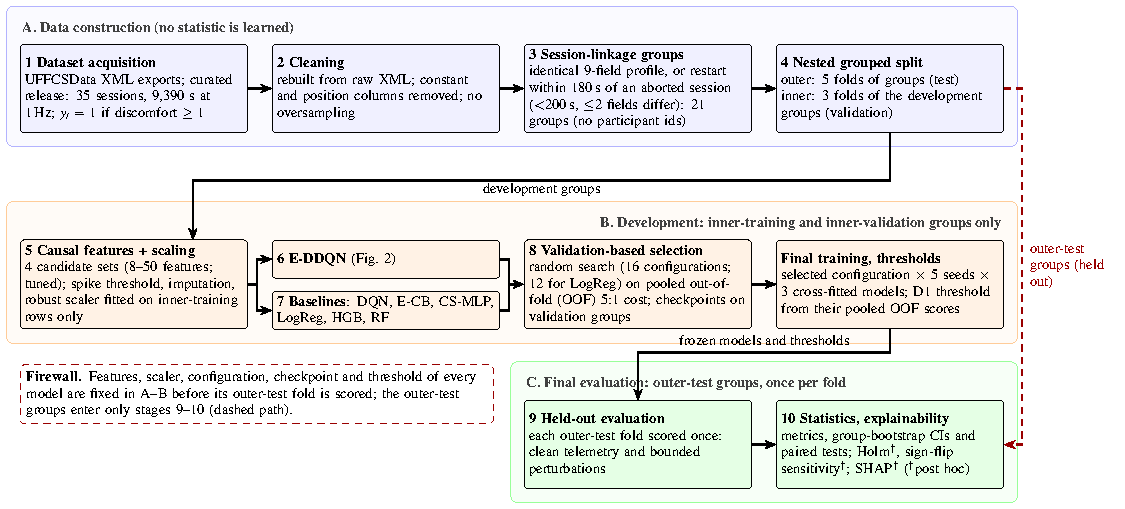
\includegraphics[width=\textwidth]{fig1_workflow.pdf}
\caption{Implemented workflow. OOF: out-of-fold; D1: validation-chosen cost-minimizing threshold; SHAP: SHapley Additive exPlanations; other abbreviations as in Section~\ref{sec:intro}. A: data construction; B: development on inner folds only (E-DDQN in Fig.~\ref{fig:arch}); C: single evaluation of each outer-test fold (protocol in Fig.~\ref{fig:protocol}). The dashed path marks the outer-test groups, which bypass every fitted step.}
\label{fig:workflow}
\end{figure*}

\subsection{Data and Target (Stages 1--2)}
\label{sec:data}
UFFCSData~\cite{porcino2019uffcsdata,porcino2022identifying,porcino2021methodology} was recorded while volunteers played a race game and a flight game in a head-mounted display. About once per second the game logged speed, acceleration, three camera-rotation components (range $[-1,1]$; the parameterization is not documented), frame rate, region of interest, configuration flags and the self-reported discomfort level (0--3: none, slight, moderate, severe)~\cite{kennedy1993ssq,porcino2019demo}. Each session also stores a pre-play Cybersickness Profile Questionnaire (CSPQ: gender, age band, VR experience, glasses, vision problems, eye dominance, flicker sensitivity). We rebuilt every input from the raw XML exports: the dataset authors' curated release (\nSessionsEval{} seated sessions, December~2019; \nSamplesEval{} samples) matches \nSessionsEval{} raw exports sample by sample and is the evaluation set; the \nSessionsDev{} October-2019 standing sessions are used only to debug code and calibrate training budgets (validation cost plateaued after 20--30 epochs, so 40 epochs were fixed).

The target is $y_t=1$ (\emph{event}) if the discomfort level at second $t$ is at least~1. The prevalence is \prevEval{} (Flight \prevFlight{}, Race \prevRace{}); grades 2--3 occur in \PHGradeRaceSevere{} of \PHGradeRaceSamples{} Race but only \PHGradeFlightSevere{} of \PHGradeFlightSamples{} Flight samples. Labels are near step functions: the binary label changes \PHLabelBinaryChanges{} times per session on average, never decreases in \PHLabelNonDecreasing{} of \PHLabelSessions{} sessions, and \nEventFreeSessions{} sessions never report discomfort. The prompting procedure is not documented, so consecutive labels are a held self-report, not independent measurements. No session was attacked: $y$ marks discomfort, not a manipulation.

\subsection{Session-Linkage Groups (Stage 3)}
\label{sec:groups}
Consecutive seconds of a session are near-duplicates with the same label, so every split must keep each session---and, as far as the data allow, each participant---on one side. The release has no participant identifier, and some participants restarted after an aborted session. We link two sessions if (a)~their nine profile fields are identical or (b)~one starts within 180\,s after an aborted session ($<200$ samples) and their profiles differ in at most two fields. The connected components are \nGroupsEval{} \emph{session-linkage groups}, the unit of every split. The rule may merge different people with the same profile, which is conservative, but cannot link one person who answered the questionnaire differently in non-consecutive sessions (Section~\ref{sec:limits}).

\subsection{Causal Features and Train-Only Preprocessing (Stage 5)}
\label{sec:features}
A feature is causal if its value at second $t$ uses only seconds $0,\dots,t$ of the same session; this was verified by recomputing all features on sessions truncated at random times. The 39 telemetry features are 13 instantaneous values (game, elapsed time, speed, acceleration, $|$acceleration$|$, the three rotation components $q_t$, $\lVert q_t-q_{t-1}\rVert$, frame rate, three region-of-interest indicators), 22 trailing-window statistics over 5\,s and 15\,s (mean, standard deviation (SD) and change of speed; mean and maximum $|$acceleration$|$; spike rate; mean and SD of rotation change; mean, minimum and drop fraction of frame rate) and 4 cumulative values (rotation change, spikes, frame drops, running mean speed). A spike is $|$acceleration$|$ above the 90th percentile of the training rows; a frame drop is a frame rate below 80\,fps. Eleven \emph{questionnaire indicators} (``profile'') encode the seven CSPQ items. The spike threshold, the imputation of the logger's zero frame rate on some first samples, and a median/interquartile-range scaler are fitted on the training rows of each inner split and applied unchanged to its validation and test rows. Constant columns (field of view and two camera flags per game, four configuration flags, posture) and the absolute position (a proxy for elapsed course distance) are removed; no oversampling or synthetic data are used. The feature set is a hyper-parameter: \emph{telemetry} (39), \emph{telemetry+profile} (50), \emph{exposure} (8 a-priori exposure descriptors: game, elapsed time, cumulative rotation change and spikes, running and 15-s mean speed, 15-s means of rotation change and $|$acceleration$|$) or \emph{exposure+profile} (19).

\subsection{Decision Formulation: Markov Decision Process or Contextual Bandit?}
\label{sec:formulation}
Each session is an episode. At second $t$ the detector observes the causal feature vector $s_t\in\mathbb{R}^d$, chooses $a_t\in\{0,1\}$ (silent, alarm) and receives $r_t=R(a_t,y_t)$ with
\begin{equation}
\begin{aligned}
R(1,1)&=+0.5, & R(0,0)&=+0.1,\\
R(0,1)&=-0.5, & R(1,0)&=-0.1.
\end{aligned}
\label{eq:reward}
\end{equation}
The next state $s_{t+1}$ is the next second of the same session; the last second is terminal ($d_t=1$). Because the telemetry was logged without an alarm in the loop, $P(s_{t+1}\mid s_t,a_t)=P(s_{t+1}\mid s_t)$, and for any $\gamma<1$
\begin{equation}
\begin{aligned}
Q^*(s,a)={}&\mathbb{E}[R(a,y_t)\mid s_t{=}s]\\
&+\underbrace{\gamma\,\mathbb{E}[(1-d_t)V^*(s_{t+1})\mid s_t{=}s]}_{\text{same for both actions}}.
\end{aligned}
\label{eq:decomp}
\end{equation}
Hence (i)~the logged-data problem is a \emph{contextual bandit}~\cite{lattimore2020bandit}: the best action maximizes the immediate expected reward for every $\gamma$. (ii)~With $p(s)=P(y=1\mid s)$ the optimal decision margin is
\begin{equation}
Q^*(s,1)-Q^*(s,0)=p(s)\,\Delta_{\mathrm{FN}}-(1-p(s))\,\Delta_{\mathrm{FP}},
\label{eq:margin}
\end{equation}
with regrets
\begin{equation}
\begin{aligned}
\Delta_{\mathrm{FN}}&=R(1,1)-R(0,1)=1.0,\\
\Delta_{\mathrm{FP}}&=R(0,0)-R(1,0)=0.2,
\end{aligned}
\label{eq:regret}
\end{equation}
so the greedy policy alarms iff $p(s)\ge\Delta_{\mathrm{FP}}/(\Delta_{\mathrm{FN}}+\Delta_{\mathrm{FP}})=1/6$: exactly the Bayes rule for costs $C_{\mathrm{FN}}:C_{\mathrm{FP}}=5:1$~\cite{elkan2001cost}. The asymmetric reward encodes an operating point, not a different objective. (iii)~Solving Eq.~\eqref{eq:margin} for $p$ maps a Q-function to a score on the nominal scale of $P(y=1\mid s)$,
\begin{equation}
\hat p(s)=\frac{\Delta Q(s)+\Delta_{\mathrm{FP}}}{\Delta_{\mathrm{FN}}+\Delta_{\mathrm{FP}}},\qquad \Delta Q(s)=Q(s,1)-Q(s,0),
\label{eq:phat}
\end{equation}
computed with each agent's own reward table ($\Delta_{\mathrm{FN}}=\Delta_{\mathrm{FP}}=2$ for the $\pm1$ reward); $\hat p$ is an uncalibrated estimate and can leave $[0,1]$. These consequences follow from known results~\cite{elkan2001cost,dudik2011efficient}; we state them because asymmetric-reward DQN detectors are usually presented without this link.

\emph{Score scale.} Class-balanced replay or minibatches (a share $1-\rho$ or one half of events instead of the training prevalence $\pi$, \SSPrevMin--\SSPrevMax) multiply the odds estimated by the scores by $k=\frac{1-\rho}{\rho}\frac{1-\pi}{\pi}$, so the nominal cut-off $\hat p\ge1/6$ corresponds to $P(y=1\mid s)\ge1/(1+5k)$: \SSEDDQNCutMin--\SSEDDQNCutMax{} for E-DDQN (approximate, since its $\gamma$ of 0.9--0.99 lets some residuals exceed the Huber threshold), \SSECBCutMin--\SSECBCutMax{} for E-CB and \SSCSMLPCutMin--\SSCSMLPCutMax{} for the balanced CS-MLP. The Huber loss with the standard DQN's $\pm1$ reward makes its $\hat p$ a nonlinear function of $P(y=1\mid s)$ (cut-off \SSDQNHuberCut{} at $\gamma=0$). These shifts affect the untuned rule D0; the primary rule D1 and the ranking metrics choose thresholds on the scores themselves, and rescaling every inner model to $P(y=1\mid s)$ changes at most \SSSensMaxChanged\,\% of D1 decisions, the cost by at most \SSSensMaxCostDelta{} and ROC-AUC by at most \SSSensMaxAucDelta{} (Supplementary Sec.~S5.12).

\emph{Episode termination and discounting.} Earlier DQN classifiers end an episode when a minority sample is misclassified~\cite{lin2020imbalanced,yang2024drlimbalanced}; a miss then also forfeits $\gamma V(s_{t+1})$, an extra $\gamma$-dependent penalty, so the problem is no longer a bandit. E-DDQN ends episodes only with the session, so Eqs.~\eqref{eq:decomp}--\eqref{eq:phat} apply. Bootstrapping ($\gamma>0$) only adds the action-independent term of Eq.~\eqref{eq:decomp} and its estimation noise; we therefore tune $\gamma\in\{0,0.5,0.9,0.99\}$ on validation data and also evaluate the separately tuned $\gamma=0$ special case (E-CB). Adaptive sequential control would require an intervention in the loop, which the data do not contain, so we make no such claim.

\subsection{E-DDQN (Stage 6)}
\label{sec:eddqn}
Fig.~\ref{fig:arch} shows E-DDQN as implemented; Table~\ref{tab:settings} lists its settings and search space. A multilayer trunk (Linear, batch or layer normalization~\cite{ioffe2015bn}, ReLU and dropout~\cite{srivastava2014dropout} except after the last layer) feeds a dueling head~\cite{wang2016dueling}, $Q(s,a)=V(s)+A(s,a)-\frac12\sum_{a'}A(s,a')$. The Double-DQN target~\cite{vanhasselt2016double} is
\begin{equation}
y_t=r_t+\gamma(1-d_t)\,Q_{\theta^-}\big(s_{t+1},\arg\max_{a'}Q_\theta(s_{t+1},a')\big),
\label{eq:ddqn}
\end{equation}
with the arg-max taken by the online network in evaluation mode ($y_t=r_t$ for $\gamma=0$). The Huber loss~\cite{huber1964robust,girshick2015fast} between $Q_\theta(s_t,a_t)$ and $y_t$ is minimized with Adam~\cite{kingma2015adam}, weight decay, gradient-norm clipping and cosine learning-rate decay~\cite{loshchilov2017sgdr}. After each update $\theta^-\leftarrow(1-\tau)\theta^-+\tau\theta$~\cite{lillicrap2016continuous}, and batch-normalization statistics are copied (all five selected E-DDQN networks used layer normalization, so this copy was inactive in the reported runs). Minibatches from the replay buffer~\cite{lin1992selfimproving} (50,000 transitions; 100,000 with full-information replay) contain a fixed share $\rho$ of non-event and $1-\rho$ of event transitions. Actions are $\varepsilon$-greedy, with an optional warm-up of random actions. With \emph{full-information replay} (tuned on/off) the action not taken is also stored with its own reward---a valid transition that the labels allow offline. Every second epoch the inner-validation groups are scored and the epoch with the lowest achievable 5:1 cost is kept (Algorithm~\ref{alg:eddqn}).

\begin{figure*}[t]
\centering
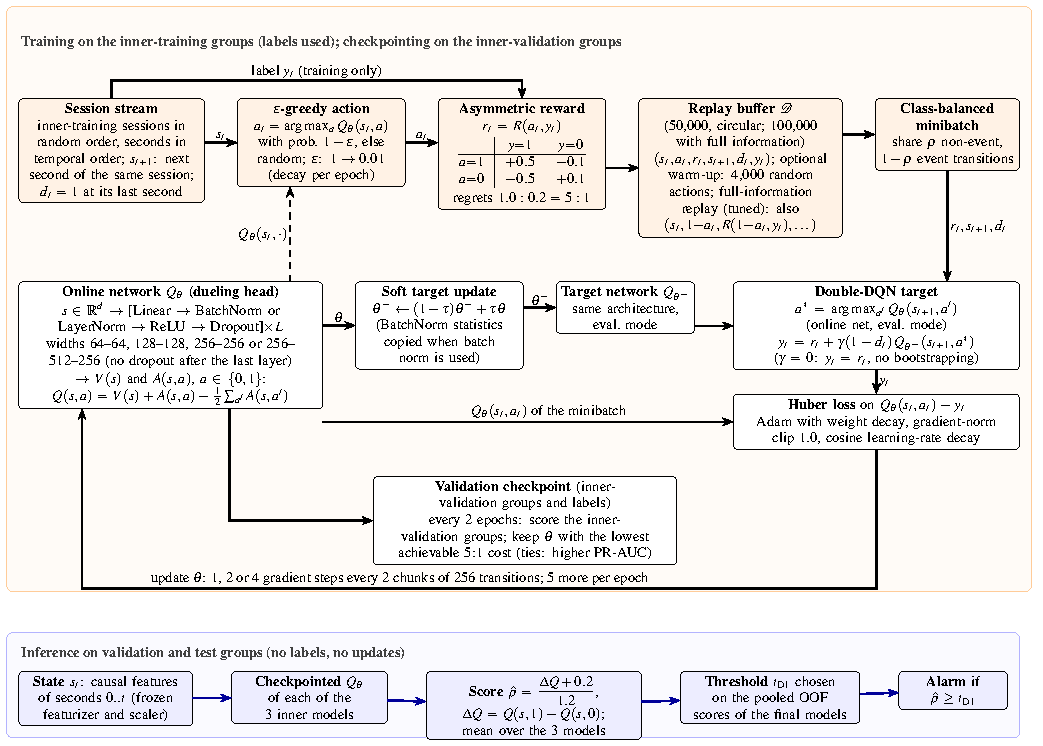
\includegraphics[width=\textwidth]{fig2_eddqn_architecture.pdf}
\caption{E-DDQN as implemented. Top (orange): training on the inner-training groups, where labels define the reward; bottom (blue): inference on validation and test groups with the checkpointed networks, the score of Eq.~\eqref{eq:phat} and the validation-chosen threshold of rule D1. Dashed: the online network selects actions; $\gamma=0$ removes the target-network path.}
\label{fig:arch}
\end{figure*}

\begin{algorithm}[t]
\caption{E-DDQN training for one inner split}
\label{alg:eddqn}
\begin{algorithmic}[1]
\small
\State Initialize $\theta$, $\theta^-\!\leftarrow\theta$, buffer $\mathcal{D}$; optional warm-up with random actions
\For{epoch $=1,\dots,40$}
  \State Concatenate training sessions in random order, each in temporal order; last second of each session terminal
  \For{each chunk of 256 consecutive transitions}
    \State $a_t\gets$ $\varepsilon$-greedy on $Q_\theta(s_t,\cdot)$;\ $r_t\gets R(a_t,y_t)$
    \State store $(s_t,a_t,r_t,s_{t+1},d_t,y_t)$ [and $(s_t,1-a_t,R(1-a_t,y_t),\dots)$ if full-information]
    \State every 2 chunks: 1, 2 or 4 updates on class-balanced minibatches with Eq.~\eqref{eq:ddqn}, Huber loss, Polyak update
  \EndFor
  \State 5 consolidation updates; decay $\varepsilon$; cosine LR step
  \State every 2 epochs: keep $\theta$ if the validation 5:1 cost improves
\EndFor
\State \Return checkpoint; score $\hat p(s)$ by Eq.~\eqref{eq:phat}
\end{algorithmic}
\end{algorithm}

\emph{Implementation checks.} An earlier implementation of this study built transitions from shuffled rows without terminal flags, stored the label as the action while rewarding a different action, and averaged only parameters into the target network. Unit tests guard against all three. On the real folds, every one of the \PVTransitions{} transitions written to the replay buffer in shortened runs of E-DDQN, E-CB and the standard DQN with each fold's selected configuration was logged: each stored reward is that of the stored action and the label of its state, each non-terminal next state is the next second of the same session, and terminal flags occur exactly at session ends (Supplementary Sec.~S8).

\subsection{Baselines (Stage 7)}
\label{sec:baselines}
Every baseline receives the same splits, candidate feature sets, search procedure and number of configurations (16; 12 for logistic regression), checkpoint rule (neural models), cross-fitting and threshold rules (Table~\ref{tab:settings}). The number of configurations is matched, not the coverage: the search spaces range from about \PHSpaceEDDQNMillion{} million configurations (E-DDQN) to \PHSpaceRF{} (random forest; Supplementary Sec.~S2.1). The \textbf{standard DQN}~\cite{mnih2015human} uses a symmetric $\pm1$ reward, a plain head, the max-operator target, periodic hard target copies and uniform replay; \textbf{E-CB} is E-DDQN with $\gamma=0$; the \textbf{CS-MLP} is a multilayer perceptron with event-weighted cross-entropy ($w=5$); \textbf{logistic regression}, \textbf{histogram gradient boosting (HGB)} and a \textbf{random forest (RF)}~\cite{pedregosa2011sklearn} use class weight 5. A weighted classifier estimates $p_w=5p/(5p+1-p)$, which is mapped back by
\begin{equation}
\hat p=\frac{p_w}{5-4p_w},
\label{eq:unweight}
\end{equation}
so that all models share the nominal scale of Eq.~\eqref{eq:phat}. \emph{Always alarm} and \emph{never alarm} are trivial references. Because exposure duration drives cybersickness~\cite{kennedy2000duration} and most selected configurations used exposure features, two exposure-time baselines were specified after the primary analysis and run under the same protocol: \textbf{Time-LR} (logistic regression on elapsed time) and \textbf{Time+game HGB}.

\begin{table}[t]
\centering
\caption{Implementation and training settings (\texttt{configs/protocol.json}, except the rows marked $^\dagger$; braces: searched values).}
\label{tab:settings}
\scriptsize
\setlength{\tabcolsep}{2.5pt}
\begin{tabular}{@{}p{0.27\columnwidth}p{0.70\columnwidth}@{}}
\toprule
Item & Setting \\
\midrule
Splits & outer \nOuter{} / inner \nInner{} stratified group folds (game $\times$ label); seeds 20261012 / 20261013--17 \\
Search & random, 16 configurations per family (LogReg 12 of 24), drawn once (sampling seed 777 + family index; training seed 777); objective: pooled OOF 5:1 cost at its best threshold, ties: area under the precision--recall curve (PR-AUC) \\
Neural (all) & feature set \{4 sets\}; trunk \{64--64, 128--128, 256--256, 256--512--256\}; dropout \{0, .1, .2, .3\}; norm \{batch, layer\}; learning rate $\eta$ \{3e-4, 1e-3, 3e-3\}, cosine to 1e-5; weight decay \{0, 1e-4, 1e-3\}; batch \{256, 512\}; 40 epochs; checkpoint every 2 epochs \\
Agents (all) & Huber loss (threshold 1), Adam, grad.-norm clip 1.0; buffer 50,000 (100,000 with full information); chunks of 256, learning step every 2 chunks with \{1, 2, 4\} updates, 5 consolidation updates per epoch; $\varepsilon$ 1.0$\rightarrow$0.01, decay \{0.90, 0.95, 0.97\}/epoch; warm-up \{0, 4,000\} \\
E-DDQN & reward Eq.~\eqref{eq:reward}; dueling; double; soft target $\tau$ \{0.005, 0.01, 0.05\}; $\gamma$ \{0, 0.5, 0.9, 0.99\}; balanced replay $\rho$ \{0.4, 0.5, 0.6\}; full-information \{off, on\} \\
E-CB & as E-DDQN with $\gamma=0$; $\rho$, full-information searched \\
DQN & $\pm1$ reward; plain head; max target; hard copy every \{10, 100, 500\} updates; $\gamma$ \{0, 0.5, 0.9, 0.99\}; uniform replay; no full-information replay \\
CS-MLP & weighted cross-entropy ($w=5$); minibatches \{uniform, balanced\} \\
LogReg & $C$ \{1e-4, \dots, 10\} (6 values) \\
HGB & $\eta$ \{.02, .05, .1\}; iterations \{50, 100, 200, 400\}; leaves \{4, 8, 16, 31\}; min.\ leaf \{20, 100, 300\}; $\ell_2$ \{0, 1, 10\} \\
RF & 300 trees; depth \{3, 5, 8, none\}; min.\ leaf \{5, 25, 100, 300\}; features \{sqrt, 0.5, 1.0\} \\
Final & 5 seeds (1000--1004) $\times$ \nInner{} cross-fitted inner models per outer fold \\
Inference$^\dagger$ & group bootstrap, 2,000 replicates (analysis code committed with the protocol); exact sign-flip test over $2^{21}$ sign patterns (post hoc) \\
Software$^\dagger$ & Python 3.13, PyTorch~\cite{paszke2019pytorch} 2.14.1 (run on the CPU), scikit-learn 1.9.1; one thread per process; full pipeline about 2.5--3.5\,h on four CPU cores; \authorinput{CPU model and memory to be added} \\
\bottomrule
\end{tabular}
\end{table}

\subsection{Evaluation Protocol and Statistics (Stages 4 and 8--10)}
\label{sec:protocol}
\label{sec:seeds}
Fig.~\ref{fig:protocol} shows the protocol; its split, search, checkpoint, threshold and seed rules were committed before any model was trained on the evaluation sessions (the post-hoc additions are marked). The \nGroupsEval{} groups are split into \nOuter{} outer folds; each serves once as test data and the rest form its development set, which is split into \nInner{} inner folds so that every development second receives one out-of-fold (OOF) validation prediction. For each family and outer fold: (1)~each configuration is trained on the three inner splits with one seed, and the one with the lowest pooled-OOF 5:1 cost $c=(5\,\mathrm{FN}+\mathrm{FP})/N$ is selected; (2)~it is retrained with five seeds, keeping the three checkpointed inner models per seed (cross-fitting), whose mean is the test score; (3)~thresholds are chosen on the pooled OOF scores of these final models: the primary rule \emph{D1} minimizes the 5:1 cost (ties: closest to $1/6$); secondary rules are \emph{D0}, the fixed cut-off $\hat p\ge1/6$ (the greedy policy for the asymmetric agents), and an OOF recall of at least 0.95. Each OOF score comes from one inner model, whereas each test score averages three, so averaging can make test scores less spread than the scores on which the threshold was chosen (checked post hoc; Section~\ref{sec:limits}, limitation (ix)); (4)~the outer-test fold is scored once, on clean and on perturbed telemetry. Checks on the real folds confirm that no session, linkage group, exact questionnaire profile, raw telemetry row or feature vector crosses a partition boundary in any of the 15 outer~$\times$~inner splits, that preprocessing is unaffected by evaluation rows, and that every configuration, checkpoint and threshold is reproduced from inner-validation data alone (Supplementary Sec.~S8). This establishes session- and linkage-group-disjoint evaluation, not participant independence.

\begin{figure*}[t]
\centering
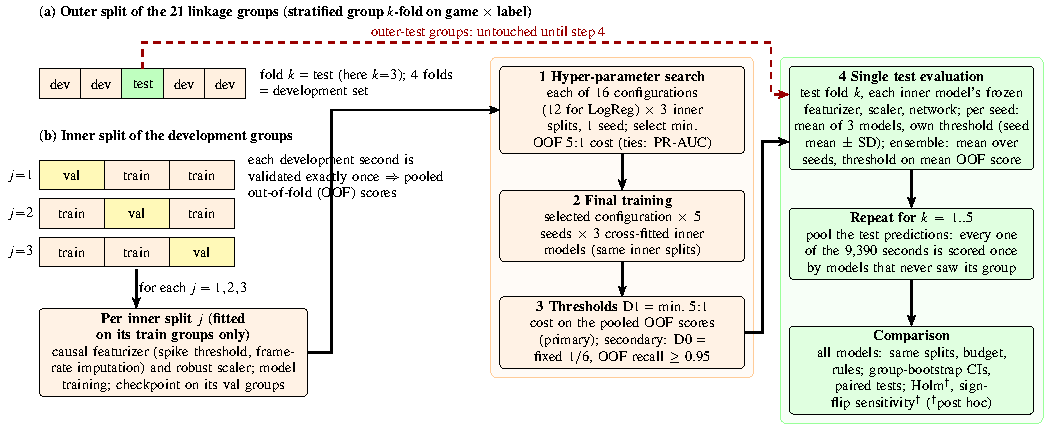
\includegraphics[width=\textwidth]{fig3_evaluation_protocol.pdf}
\caption{Nested, session-linkage-grouped evaluation protocol, applied identically to every model. Within each outer fold, all fitting, selection, checkpointing and thresholding use inner folds of the development groups; the outer-test groups are used once, in step~4.}
\label{fig:protocol}
\end{figure*}

\emph{Seed means and seed ensemble.} We report mean~$\pm$~SD over the five seeds. Analyses that need one prediction per sample (paired tests, confidence intervals, comparison with always alarming, event-level metrics, matched operating points, perturbations, cost curves) use the \emph{seed ensemble}, the mean score over seeds thresholded on the mean OOF score; this was fixed in the evaluation code before the evaluation. The two can differ: E-DDQN's ensemble cost is \PHEnsEDDQNCost{} against a seed mean of \EDDQNCostCostMean, the standard DQN's \PHEnsDQNCost{} against \DQNCostCostMean. No seed was selected or discarded.

\emph{Metrics and inference.} We report recall, specificity, balanced accuracy, Matthews correlation coefficient (MCC)~\cite{chicco2020mcc}, missed events, false positives, the 5:1 cost, ROC-AUC and PR-AUC~\cite{saito2015pr} (further metrics in Supplementary Sec.~S3.1) and event-level alarm fractions. Confidence intervals (CIs) are percentile intervals of a bootstrap over the \nGroupsEval{} linkage groups (2,000 replicates); they describe the sampling of test groups given the trained models, not retraining variability beyond the five seeds. The primary paired test is a group bootstrap of the seed-ensemble cost difference, $p=2\min\{\Pr(\Delta^*\le0),\Pr(\Delta^*\ge0)\}$ (resolved to about 0.001); it was implemented in the analysis code committed with the frozen protocol and yields effect size, CI and $p$-value from one distribution. An exact group sign-flip test over all $2^{21}$ sign patterns, added after a pre-submission review, is the sensitivity analysis. Every comparison is reported as an effect size with its 95\,\% CI and Holm-adjusted~\cite{holm1979simple} $p$-values, and a difference is treated as firmly established only if it is significant under both procedures. With \nGroupsEval{} unequal groups, cluster-bootstrap inference is approximate and can be anti-conservative~\cite{cameron2008bootstrap}, so $p$-values between 0.01 and 0.05 are read as approximate. Sample-level McNemar tests~\cite{mcnemar1947,dietterich1998tests} are secondary because consecutive seconds are dependent.

\emph{Post-hoc analyses} (Supplementary Sec.~S5). The following were specified after the primary results were known and committed before being run, unless stated otherwise: the exposure-time baselines; Holm adjustment of the six comparisons with E-DDQN; comparison with always alarming (its Holm adjustment added without prior commitment); session-level bootstrap and leave-one-group-out jackknife; validation-chosen cost curves over cost ratios $R$ from 1 to 20; within-fold ROC-AUC, sign-flip tests and feature-set tallies (after review, with all results known); a \emph{search-draw experiment}, specified with three decision rules and committed before it was run, which re-tunes E-DDQN and the standard DQN with two further random draws of 16 configurations and one exposure-only draw (Supplementary Sec.~S5.11); the descriptive score-scale calculation above (added in the final pre-submission check); and a threshold-scale check of the D1 results (specified and committed before it was run; Supplementary Sec.~S9.10). The paired comparisons of the exposure-time baselines with the primary models and the Q-value-scale diagnostic were added without prior commitment.

\subsection{Telemetry-Perturbation Stress Tests and Explainability}
\label{sec:threat}
\label{sec:shap}
The motivating threats degrade frame pacing, distort camera or locomotion motion, or manipulate the field of view~\cite{odeleye2021framerate,tseng2022dark,kundu2025securing}. The data contain no attacked sessions, so we use bounded, synthetic changes of the outer-test telemetry as a stress test of which inputs the detectors use; features are recomputed with the frozen featurizer and scaler, and labels are unchanged. The 24 variants, fixed before evaluation, are frame-rate capping, orientation jitter, speed up-scaling and acceleration-spike injection at three strengths, applied to the whole session or one 60-s window (values and bounds in Supplementary Sec.~S4.1; the 60- and 45-fps caps lie below every Flight frame rate after the first second, \SSFpsFlightMin--\SSFpsFlightMax\,fps). Field-of-view manipulation is not evaluated because it never varies within a game. An adaptive adversary with label knowledge picks, per session, among 17 whole-session variants (including five ``hiding'' manipulations that mask stress signals: speed down-scaling, orientation smoothing, frame-rate restoration) the one that minimizes alarms on event seconds or maximizes alarms on non-event seconds; these are lower bounds, weaker than gradient-based attacks~\cite{kundu2025securing,ahmed2025adversarialvr}. Post hoc, SHAP values (SHapley Additive exPlanations)~\cite{lundberg2017shap} of the decision margin $\Delta Q$ are computed for one separately retrained E-DDQN model per outer fold with the expected-gradients estimator (DeepExplainer~\cite{shrikumar2017deeplift} failed its additivity check on the layer-normalized networks; Supplementary Sec.~S9.8).
% ---- end sections_v2/s3_method

% ---- begin sections_v2/s5_results
\section{Results}
\label{sec:results}

\subsection{Effect of the Split Protocol}
\label{sec:leak}
Table~\ref{tab:leak} evaluates the same 21 raw columns under three protocols with an untuned gradient-boosting classifier, quantifying a known pitfall~\cite{kapoor2023leakage,kaufman2012leakage} on these data. Oversampling every discomfort grade to 5,243 samples before a 70/15/15 row split, the protocol of the earlier version of this study, gives \LeakOldAcc\,\% accuracy and ROC-AUC \LeakOldRocAuc; \LeakDupPct\,\% of the positive test rows have an exact duplicate in training. A row-level split without oversampling still gives ROC-AUC \LeakRowRocAuc, whereas a session-grouped split gives \LeakGrpRocAuc{} (MCC \LeakGrpMCC). The earlier E-DDQN implementation behaves alike (MCC \OrigOldMCC{} vs.\ \OrigGrpMCC). Near-perfect scores on these data thus measure recognition of seen sessions, without any RL; all further results use the grouped protocol of Fig.~\ref{fig:protocol}.

\begin{table*}[t]
\centering
\caption{Effect of the evaluation protocol on the same data (21 raw columns; test-split metrics). ``Proxy'': reconstruction of the earlier protocol, whose 41-feature input files were not available.}
\label{tab:leak}
\resizebox{\textwidth}{!}{% ---- begin generated/tab_leakage.tex
\begin{tabular}{llccccc}
\toprule
Model & Evaluation protocol & Acc. & Recall & Spec. & MCC & ROC-AUC \\
\midrule
HGB & Oversample to 5,243/grade, then 70/15/15 row split (earlier protocol) & 97.6 & 99.8 & 91.0 & 0.935 & 0.995 \\
HGB & Row-level random split, no oversampling & 95.3 & 94.1 & 96.3 & 0.905 & 0.992 \\
HGB & Grouped 5-fold split (session-linkage groups) & 52.2 & 33.6 & 66.9 & 0.005 & 0.523 \\
E-DDQN (earlier code) & Earlier script, earlier protocol (proxy) & 95.2 & 99.2 & 83.1 & 0.870 & -- \\
E-DDQN (earlier code) & Earlier script, grouped split (proxy) & 41.1 & 92.1 & 7.7 & $-$0.004 & -- \\
\bottomrule
\end{tabular}
% ---- end generated/tab_leakage.tex
}
\end{table*}

\subsection{Session-Grouped Comparison under the 5:1 Cost (RQ2)}
\label{sec:main}
Table~\ref{tab:main} gives every model's result, with thresholds chosen on validation groups only. Two facts dominate. First, discrimination is weak once sessions and groups are not shared: the best primary ROC-AUC is \HGBCostRocAucMean{} (HGB) and \RFCostRocAucMean{} (RF), and the best PR-AUC \DQNCostPrAucMean{} (DQN) against a prevalence of 0.44. Second, under a 5:1 cost every cost-optimal operating point lies near ``always alarm'' (cost \AlwaysCost): recall is high, but \DOneFPRMin--\DOneFPRMax\,\% of non-event seconds trigger an alarm. The random forest has the lowest cost (seed mean \RFCostCostMean$\pm$\RFCostCostSD; ensemble \PHEnsRFCost; point estimates, differences among supervised models not tested).

With its primary search draw (draw~1), E-DDQN has the highest cost and lowest ROC-AUC of the \nModels{} primary models (point estimates; tests in Section~\ref{sec:stats}): cost \EDDQNCostCostMean$\pm$\EDDQNCostCostSD{} (ensemble \PHEnsEDDQNCost), recall \EDDQNCostRecallMean\,\%, specificity \EDDQNCostSpecMean\,\%, ROC-AUC \EDDQNCostRocAucMean{} (ensemble \EDDQNCostRocAucEns, 95\,\% CI \EDDQNCIRocAucLo{} to \EDDQNCIRocAucHi, which includes chance). Its seed-ensemble cost exceeds the random forest's in \PHFoldsEDDQNWorseRF{} of 5 outer folds, by \PHFoldDiffEDDQNRFMin{} to \PHFoldDiffEDDQNRFMax. The standard DQN reaches cost \DQNCostCostMean{} and ROC-AUC \DQNCostRocAucMean, E-CB \ECBCostCostMean{} and \ECBCostRocAucMean.

\begin{table*}[t]
\centering
\caption{Session-grouped comparison (rule D1; \nSamplesEval{} outer-test samples; recall, specificity, balanced accuracy in \%). Left: mean~$\pm$~SD over five seeds. Right: seed ensemble, used for all paired tests and confidence intervals; FN and FP are exact counts. Bold: proposed model and lowest primary cost. HGB, logistic regression and the post-hoc baselines are deterministic (SD = 0). Further metrics: Supplementary Sec.~S3.1.}
\label{tab:main}
\resizebox{\textwidth}{!}{% ---- begin generated/tab_main_D1_with_posthoc.tex
\begin{tabular}{lccccccc|ccccc}
\toprule
 & \multicolumn{7}{c|}{Mean $\pm$ SD over five seeds} & \multicolumn{5}{c}{Seed ensemble (paired tests)} \\
Model & Recall & Spec. & Bal.\ acc. & MCC & Cost$_{5:1}$ & ROC-AUC & PR-AUC & Recall & Spec. & Cost$_{5:1}$ & FN & FP \\
\midrule
\textbf{E-DDQN} & 93.4$\pm$2.5 & 7.4$\pm$2.7 & 50.4$\pm$1.2 & 0.016$\pm$0.054 & 0.663$\pm$0.048 & 0.538$\pm$0.016 & 0.483$\pm$0.019 & 90.4 & 8.1 & 0.726 & 400 & 4,820 \\
E-CB & 97.1$\pm$2.9 & 8.4$\pm$2.8 & 52.8$\pm$1.2 & 0.122$\pm$0.052 & 0.575$\pm$0.055 & 0.653$\pm$0.011 & 0.562$\pm$0.006 & 96.6 & 14.6 & 0.552 & 140 & 4,480 \\
DQN & 95.2$\pm$2.7 & 14.5$\pm$4.9 & 54.8$\pm$1.6 & 0.158$\pm$0.038 & 0.584$\pm$0.040 & 0.661$\pm$0.013 & 0.595$\pm$0.022 & 96.9 & 16.3 & 0.536 & 129 & 4,391 \\
CS-MLP & 99.4$\pm$0.7 & 2.8$\pm$1.9 & 51.1$\pm$0.8 & 0.072$\pm$0.049 & 0.557$\pm$0.012 & 0.644$\pm$0.018 & 0.521$\pm$0.022 & 99.4 & 6.1 & 0.537 & 23 & 4,925 \\
LogReg & 99.1$\pm$0.0 & 8.1$\pm$0.0 & 53.6$\pm$0.0 & 0.167$\pm$0.000 & 0.532$\pm$0.000 & 0.626$\pm$0.000 & 0.576$\pm$0.000 & 99.1 & 8.1 & 0.532 & 36 & 4,817 \\
HGB & 97.0$\pm$0.0 & 14.6$\pm$0.0 & 55.8$\pm$0.0 & 0.197$\pm$0.000 & 0.543$\pm$0.000 & 0.692$\pm$0.000 & 0.593$\pm$0.000 & 97.0 & 14.6 & 0.543 & 124 & 4,479 \\
RF & 98.5$\pm$0.3 & 18.2$\pm$0.7 & 58.3$\pm$0.3 & 0.266$\pm$0.004 & \textbf{0.491$\pm$0.003} & 0.688$\pm$0.002 & 0.548$\pm$0.001 & 98.7 & 18.3 & \textbf{0.485} & 54 & 4,281 \\
\midrule
\multicolumn{13}{l}{\emph{Post-hoc exposure-time baselines (added after the primary analysis)}} \\
Time-LR (elapsed time) & 96.7$\pm$0.0 & 15.0$\pm$0.0 & 55.8$\pm$0.0 & 0.194$\pm$0.000 & 0.548$\pm$0.000 & 0.704$\pm$0.000 & 0.605$\pm$0.000 & 96.7 & 15.0 & 0.548 & 138 & 4,457 \\
Time+game HGB & 97.4$\pm$0.0 & 17.6$\pm$0.0 & 57.5$\pm$0.0 & 0.239$\pm$0.000 & 0.517$\pm$0.000 & 0.676$\pm$0.000 & 0.550$\pm$0.000 & 97.4 & 17.6 & 0.517 & 107 & 4,319 \\
\midrule
Always alarm & 100.0 & 0.0 & 50.0 & 0.000 & 0.558 & -- & -- & 100.0 & 0.0 & 0.558 & 0 & 5,243 \\
Never alarm & 0.0 & 100.0 & 50.0 & 0.000 & 2.208 & -- & -- & 0.0 & 100.0 & 2.208 & 4,147 & 0 \\
\bottomrule
\end{tabular}
% ---- end generated/tab_main_D1_with_posthoc.tex
}
\end{table*}

\emph{Exposure-time baselines (post hoc).} Time-LR, a logistic regression on elapsed time alone, reaches ROC-AUC \PHTimeLRRocAucMean{} (Fig.~\ref{fig:roc}). Computed within each outer fold and averaged (\emph{within-fold ROC-AUC}, which avoids pooling the scores of five fold-specific models), the random forest is slightly higher (\PHWfRFAuc{} vs.\ \PHWfTimeLRAuc) and E-DDQN lowest (\PHWfEDDQNAuc). Time-LR's ROC-AUC does not differ significantly from the random forest's (difference \PHTimeLRvsRFAuc, CI \PHTimeLRvsRFAucLow{} to \PHTimeLRvsRFAucHigh), and the wide interval does not establish equivalence either. At the 5:1 operating point the random forest has a lower cost than Time-LR (\PHEnsRFCost{} vs.\ \PHEnsTimeLRCost; group bootstrap $p=$\,\PHTimeLRvsRFCostP, sign-flip $p=$\,\PHSfTimeLRvsRFP; approximate), so the evidence that its additional inputs help is suggestive, not conclusive. Time+game HGB (cost \PHTimeHGBCostMean, ROC-AUC \PHTimeHGBRocAucMean) does not differ significantly from the random forest either (cost $p=$\,\PHTimeHGBvsRFCostP, ROC-AUC $p=$\,\PHTimeHGBvsRFAucP). Time-LR ranks seconds better than the primary E-DDQN (ROC-AUC difference \PHTimeLRvsEDDQNAuc, CI \PHTimeLRvsEDDQNAucLow{} to \PHTimeLRvsEDDQNAucHigh). No primary model was shown to discriminate better than a population onset curve---a risk of discomfort that rises with time in the session---as long documented for exposure duration~\cite{kennedy2000duration}; modest gains remain possible within the wide intervals.

\begin{figure}[t]
\centering
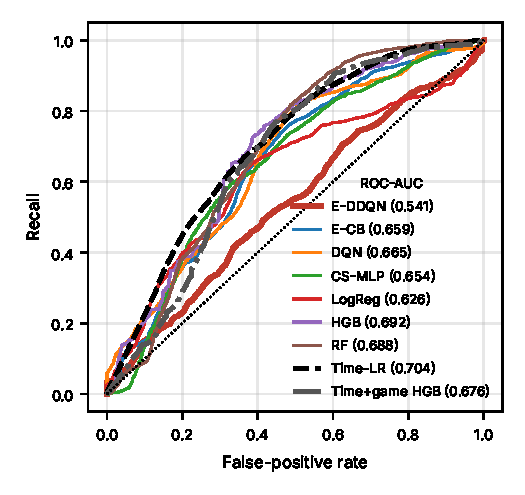
\includegraphics[width=\columnwidth]{fig4_roc.pdf}
\caption{ROC curves of the seed-ensemble scores, pooled over the outer-test folds, for the primary models and the exposure-time baselines (dashed). Legend: ensemble ROC-AUC.}
\label{fig:roc}
\end{figure}

\subsection{Statistical Comparison}
\label{sec:stats}
Table~\ref{tab:paired} compares E-DDQN with each primary model on identical test samples (seed ensembles). E-DDQN's ensemble cost exceeds the others' by \PairDOneECBCostDiff{} to \PairDOneRFCostDiff; these differences are larger than those of seed means (\PHMeanDiffDQN{} to \PHMeanDiffRF) because E-DDQN's ensemble is worse than its average seed. After Holm adjustment, only the difference from the random forest is significant under the primary group bootstrap (\PairDOneRFCostDiff, 95\,\% CI \PairDOneRFCostLo{} to \PairDOneRFCostHi; $p=$\,\PHHolmRF); the other five adjusted $p$-values lie between \PHHolmECB{} and \PHHolmHGB, and the difference from the standard DQN (\PairDOneDQNCostDiff) is not significant (unadjusted $p=$\,\PairDOneDQNPboot). The sign-flip sensitivity analysis gives $p=$\,\PHSfRFHolm{} (Holm) for the random-forest comparison. The direction is stable---the session-level bootstrap gives the same pattern (Holm $p=$\,\PHSesRFHolm) and no leave-one-group-out deletion changes the sign (\PHJkEDDQNvsRFMin{} to \PHJkEDDQNvsRFMax)---but because the difference is significant under the primary procedure only, it is not firmly established, and we do not conclude that the random forest is superior.

Against always alarming, no model's cost difference is significant after Holm adjustment with linkage groups as units (random forest \PHAlwRFGrp, CI \PHAlwRFGrpLow{} to \PHAlwRFGrpHigh, adjusted $p=$\,\PHAlwRFGrpHolm; E-DDQN \PHAlwEDDQNGrp, adjusted $p=$\,\PHAlwEDDQNGrpHolm). This reflects the strength of the evidence, not demonstrated equivalence; resampling sessions instead, which ignores dependence between linked sessions, leaves the random forest's advantage significant (adjusted $p=$\,\PHAlwRFSesHolm, approximate).

\begin{table*}[t]
\centering
\caption{Paired comparisons with E-DDQN (A) on the same \nSamplesEval{} test samples (seed ensembles, rule D1). $b$: A correct, B wrong; $c$: A wrong, B correct. $\Delta$Cost: difference of seed-ensemble costs; CI and $p_{\text{group}}$ from 2,000 group-bootstrap replicates (unadjusted; Holm-adjusted values in the text); $p_{\text{exact}}$: sample-level McNemar test, which ignores within-session dependence.}
\label{tab:paired}
\footnotesize
% ---- begin generated/tab_paired_D1.tex
\begin{tabular}{lcccccccc}
\toprule
B (vs. A = E-DDQN) & $b$ & $c$ & err$_A$ & err$_B$ & $\chi^2_{cc}$ & $p_{\text{exact}}$ & $\Delta$Cost$_{5:1}$ (A$-$B) [95\% CI] & $p_{\text{group}}$ \\
\midrule
E-CB & 299 & 899 & 5,220 & 4,620 & 299.5 & $<$0.001 & +0.175 [+0.016, +0.448] & 0.014 \\
DQN & 297 & 997 & 5,220 & 4,520 & 377.6 & $<$0.001 & +0.190 [$-$0.017, +0.493] & 0.079 \\
CS-MLP & 402 & 674 & 5,220 & 4,948 & 68.3 & $<$0.001 & +0.190 [+0.005, +0.485] & 0.039 \\
LogReg & 389 & 756 & 5,220 & 4,853 & 117.0 & $<$0.001 & +0.194 [+0.011, +0.477] & 0.026 \\
HGB & 203 & 820 & 5,220 & 4,603 & 370.9 & $<$0.001 & +0.183 [+0.011, +0.460] & 0.035 \\
RF & 293 & 1,178 & 5,220 & 4,335 & 531.2 & $<$0.001 & +0.242 [+0.052, +0.528] & 0.001 \\
\bottomrule
\end{tabular}
% ---- end generated/tab_paired_D1.tex

\end{table*}

\subsection{Operating Points and Cost Ratios}
\label{sec:op}
With the untuned rule D0 (for E-DDQN the greedy policy, an effective cut-off of \SSEDDQNCutMin--\SSEDDQNCutMax{} on $P(y=1\mid s)$) E-DDQN reaches recall \EDDQNBayesRecallMean\,\% at specificity \EDDQNBayesSpecMean\,\% (cost \EDDQNBayesCostMean), the random forest \RFBayesRecallMean\,\% at \RFBayesSpecMean\,\% (\RFBayesCostMean); under a validation recall of at least 0.95 the random forest again has the lowest cost (\RFRecCostMean; E-DDQN \EDDQNRecCostMean; Supplementary Sec.~S9.3). At validation-matched recall targets, E-DDQN's thresholds transfer worst (Supplementary Sec.~S9.4). Since the reward encodes the same operating point as a cost-weighted classifier (Eq.~\eqref{eq:margin}), on these data it provided no advantage that cost weighting plus a validation-chosen threshold did not.

The cost curves (Fig.~\ref{fig:costcurves}) show that this negative result does not depend on the 5:1 ratio. At $R=1.5$--2, the relative costs of all models except E-DDQN lie between \PHCcLowRMin{} and \PHCcLowRMax; as $R$ grows, always alarming becomes nearly optimal and models that still miss events rise above 1 (at $R=20$: E-DDQN \PHCcEDDQNTwenty, DQN \PHCcDQNTwenty). The lowest relative cost over all models and ratios is \PHCcMinAll{} (random forest, $R=\PHCcMinAllRatio$), so no model removes more than about \PHCcMinAllReduction\,\% of the cost of the better trivial policy at any ratio (point estimates).

\begin{figure}[t]
\centering
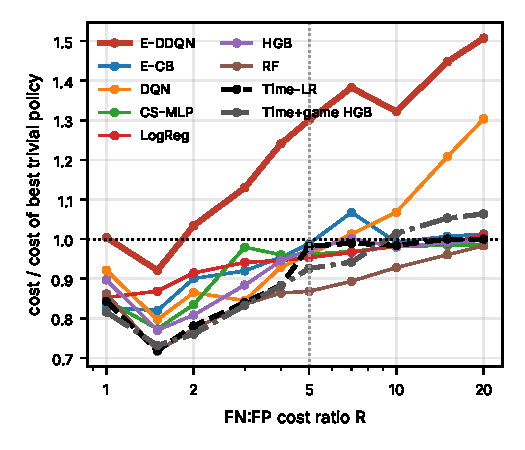
\includegraphics[width=\columnwidth]{fig5_cost_curves.pdf}
\caption{Validation-chosen cost curves (post hoc): for each cost ratio $R$, the threshold minimizing $R\,\mathrm{FN}+\mathrm{FP}$ on validation predictions is applied to the test fold; the seed-ensemble test cost is divided by that of the better trivial policy. Values below 1 beat both trivial policies; dotted line: $R=5$.}
\label{fig:costcurves}
\end{figure}

\emph{Event level.} At the cost-optimal operating points every model flags almost every session: E-DDQN alarms on \EDDQNEvFreeAlarm\,\% of the seconds of the \nEventFreeSessions{} event-free sessions and \EDDQNEvPreAlarm\,\% of pre-onset seconds (random forest \RFEvFreeAlarm\,\% and \RFEvPreAlarm\,\%), so events are ``detected'' with zero median delay by construction, not by discrimination.

\subsection{Why E-DDQN Under-Performs in the Primary Analysis}
\label{sec:why}
Validation selected $\gamma=$ \EDDQNGammas{} for E-DDQN's five folds and the questionnaire indicators in \EDDQNnProfile{} of 5 folds.

\emph{Search-draw experiment (specified and committed before it was run).} E-DDQN and the standard DQN were re-tuned under the full protocol with two further random draws of 16 configurations and one exposure-only draw, with three decision rules fixed in advance (R1: is the E-DDQN--DQN cost comparison overturned? R2: does E-DDQN's result depend on the draw? R3: does restricting both to exposure features close their ranking gap?). In none of the three full-space draws or the exposure-only draw did E-DDQN have a significantly lower cost than the DQN (seed-ensemble differences \SDCostDiffMin{} to \SDCostDiffMax; smallest $p=$\,\SDCostPMin, in draw~1; R1). E-DDQN's own result depended strongly on the draw (R2): seed-mean cost \SDEDDQNCostMin--\SDEDDQNCostMax{} and within-fold ROC-AUC \SDEDDQNWfMin, the lowest of the primary models, to \SDEDDQNWfMax, close to the highest (RF \PHWfRFAuc; not tested); the DQN varied less (\SDDQNWfMin--\SDDQNWfMax). The ranking of the two agents reversed: the DQN ranked seconds better with draw~1 (unadjusted $p=$\,\SDPairOneAucP, approximate), E-DDQN with draw~2 (unadjusted $p=$\,\SDPairTwoAucP). Restricted to exposure features, E-DDQN's within-fold ROC-AUC (\SDEDDQNExposureWfAuc) was within \SDExposureGap{} of the DQN's (R3).

\emph{Search draw and selection (exploratory, post hoc).} Each family's configurations were drawn once and reused in every outer fold; E-DDQN's primary draw offered only \PHDrawExposureEDDQN{} exposure-only configurations (DQN \PHDrawExposureDQN; Supplementary Sec.~S5.10), and validation selected configurations with questionnaire indicators in \EDDQNnProfile{} of 5 folds. The selection criterion is nearly flat near always alarming (\PHSelCostMin--\PHSelCostMax{} for the selected configurations vs.\ \AlwaysCost), so with noisy training curves and validation checkpointing configurations can look best on validation folds by chance~\cite{varma2006bias}. The \emph{selection optimism}, outer-test cost minus the inner-validation cost at selection, is \EDDQNOptGap{} for E-DDQN and \RFOptGap--\ECBOptGap{} for the other models (Supplementary Sec.~S9.5).

\emph{Questionnaire indicators (exploratory).} Across the seven primary models, the \PHFsProfile{} selected configurations with questionnaire indicators rank worse within folds than the \PHFsNoProfile{} without them (deviation from the fold mean \PHFsDevProfile{} vs.\ \PHFsDevNoProfile; without E-DDQN \PHFsDevProfileExE{} vs.\ \PHFsDevNoProfileExE; Supplementary Sec.~S5.9). With \nGroupsEval{} groups such indicators may fit group-level label rates that do not transfer; feature sets were selected, not assigned, so this suggests but does not establish a cause.

\emph{Bootstrapping.} With E-DDQN's configurations fixed, $\gamma=0$ raises ROC-AUC only from \EDDQNCostRocAucMean{} to \AblGammaZeroCostRocAuc{} (Table~\ref{tab:ablation}), and in draw~2 E-DDQN reached its best ranking with $\gamma=0.99$ in \SDEDDQNDrawTwoStrongGammaFolds{} of 5 folds. Q-values stay finite but exceed the return bound $r_{\max}/(1-\gamma)$ by up to a factor of \PHQRatioMaxEDDQN{} (Supplementary Sec.~S5.6).

Together these results suggest that sensitivity to the search draw, combined with noisy validation-based selection, contributes substantially to E-DDQN's weak primary result. They do not isolate a single cause---draw, feature sets, discount factors and other hyper-parameters varied together---and they do not show that any E-DDQN component helps a configuration that ranks well.

\subsection{Component Ablation and Reward Ratio}
\label{sec:ablation}
% ---- begin sections_v2/s5b_ablation
Table~\ref{tab:ablation} removes or changes one component of E-DDQN at a time while keeping the configuration selected for each outer fold fixed (five seeds; same protocol). No formal test was performed, so the differences below are point estimates. Because the selected configurations already used no warm-up in four of the five folds, the ``no warm-up'' variant differs from the full model only in the remaining fold. This analysis and the reward-ratio analysis below hold E-DDQN's primary (draw-1) configurations fixed, which rank weakly (Section~\ref{sec:why}); they cannot show whether a component helps a configuration that ranks well. Every variant ranks seconds only weakly (ROC-AUC \AblSoftCostRocAuc--\AblGammaZeroCostRocAuc, where 0.5 is chance). No single change moves the cost by more than about one seed standard deviation of the full model (\EDDQNCostCostMean$\pm$\EDDQNCostCostSD). The lowest cost is obtained by \emph{replacing} the asymmetric reward with the symmetric $\pm1$ reward (\AblAsymCostCost) and the highest ROC-AUC by switching off bootstrapping ($\gamma=0$; \AblGammaZeroCostRocAuc); hard target copies (\AblSoftCostCost), no dueling head (\AblDuelCostCost), uniform replay (\AblBalCostCost), no warm-up (\AblWarmCostCost) and toggling full-information replay (\AblFullCostCost) leave the cost essentially unchanged, and removing the double estimator slightly increases it (\AblDoubleCostCost). None of these components can be credited with a gain in safety or accuracy. Every variant is scored on the same nominal implied-probability scale and thresholded with the same rules, so the reward table can act only through the learned scores; at the fixed cut-off $\hat p\ge1/6$ (rule D0) the symmetric-reward variant is not worse either (cost \AblAsymBayesCost{} vs.\ \EDDQNBayesCostMean), although the effective position of that cut-off on $P(y=1\mid s)$ differs between the variants (Section~\ref{sec:formulation}).

\begin{table*}[t]
\centering
\caption{Leave-one-component-out ablation of E-DDQN (selected configuration per outer fold held fixed; rule D1; mean over 5 seeds, cost $\pm$ SD). The no-warm-up variant changes only the one fold whose selected configuration used warm-up.}
\label{tab:ablation}
\footnotesize
% ---- begin generated/tab_ablation_D1.tex
\begin{tabular}{lccccc}
\toprule
Variant & Recall & Spec. & Cost$_{5:1}$ & ROC-AUC & PR-AUC \\
\midrule
Full E-DDQN (selected) & 93.4 & 7.4 & 0.663$\pm$0.048 & 0.538 & 0.483 \\
\midrule
full-information replay toggled & 93.7 & 5.4 & 0.667$\pm$0.106 & 0.563 & 0.500 \\
symmetric $\pm$1 reward instead of asymmetric & 94.8 & 8.6 & 0.625$\pm$0.038 & 0.572 & 0.517 \\
uniform instead of class-balanced replay & 94.3 & 4.3 & 0.660$\pm$0.045 & 0.554 & 0.486 \\
no double estimator (max-operator target) & 93.1 & 5.3 & 0.681$\pm$0.086 & 0.543 & 0.491 \\
no dueling head & 94.6 & 5.8 & 0.644$\pm$0.059 & 0.559 & 0.494 \\
hard target copy every 10 updates & 94.9 & 6.5 & 0.634$\pm$0.043 & 0.529 & 0.472 \\
no warm-up & 93.8 & 7.1 & 0.656$\pm$0.049 & 0.547 & 0.497 \\
$\gamma=0$ (contextual bandit) & 94.4 & 6.4 & 0.645$\pm$0.070 & 0.576 & 0.510 \\
\bottomrule
\end{tabular}
% ---- end generated/tab_ablation_D1.tex

\end{table*}
% ---- end sections_v2/s5b_ablation

Varying the reward's regret ratio from 1:1 to 10:1 with E-DDQN's configurations fixed moves the greedy policy along the trade-off as Eq.~\eqref{eq:margin} predicts (recall \RatioArgOneRecall\,\% at 1:1, \RatioArgFiveRecall\,\% at 5:1, \RatioArgOneZeroRecall\,\% at 10:1), but once the threshold is chosen on validation data all ratios end at similar costs (\RatioTunedOneCost--\RatioTunedOneZeroCost; within one seed SD, untested; Supplementary Sec.~S9.6): the ratio sets the default operating point, not the discrimination.

\subsection{Telemetry-Perturbation Stress Test (RQ3)}
\label{sec:attack}
Under the whole-session perturbations, \AttAucFracSmall\,\% of the model--scenario ROC-AUC values change by less than 0.03 and none by more than \AttAucMaxAbsChange{} (Supplementary Sec.~S9.7). This feature-space stress test gives no evidence of robustness: \PHFsExposure{} of \PHFsTotal{} selected configurations use exposure features, which the perturbations barely touch, and a shift applied to every session alike need not reorder scores. At fixed thresholds the adaptive adversary lowers recall on event seconds by \AttEvasionDropMin--\AttEvasionDropMax{} percentage points and raises false-positive rates to \EDDQNAttWorstFPR--100\,\% (Supplementary Sec.~S4.3). SHAP attributions of E-DDQN's $\Delta Q$ are dominated by \ShapTopFive{} (Supplementary Sec.~S9.8): exposure and questionnaire inputs rather than instantaneous telemetry, consistent with the exposure-time baselines; since the primary E-DDQN ranks near chance, they describe what it uses, not a validated signal.
% ---- end sections_v2/s5_results

% ---- begin sections_v2/s6_discussion
\section{Discussion}
\label{sec:discussion}

\subsection{What the Results Support}
\emph{Evaluation.} On these data the split protocol, not the model, decides whether scores look near-perfect; accuracy figures on gameplay cybersickness data should be read together with the split protocol.

\emph{RQ1.} On logged data the asymmetric reward encodes a cost-sensitive operating point: under the natural class mix the greedy policy is the 5:1 Bayes rule, and class-balanced replay shifts it. Empirically the ratio moved the default operating point but not the discrimination, and replacing the asymmetric reward with the symmetric one lowered rather than raised E-DDQN's cost as a point estimate (Section~\ref{sec:ablation}). The evidence therefore does not support a benefit of the asymmetric reward beyond what cost weighting and a validation-chosen threshold provide.

\emph{RQ2.} E-DDQN did not have a significantly lower 5:1 cost than the standard DQN with any of three search draws, and the two agents' ranking reversed between draws, so neither is consistently better. With its primary draw its seed-ensemble cost was higher than the random forest's, significantly under the primary procedure but not under the sensitivity analysis, so this is not firmly established. No primary model ranked seconds significantly better than elapsed time, and no model meets a safety-prioritized target.

\emph{RQ3.} The small effect of bounded perturbations on ranking reflects which inputs the selected configurations use; at fixed thresholds an adaptive adversary still changes decisions. These feature-space stress tests say nothing about real rendering attacks.

\subsection{Is E-DDQN Reinforcement Learning?}
With logged data the alarm cannot influence later telemetry, so the problem is a contextual bandit. E-DDQN remains a valid value-based learner of a cost-sensitive policy, but bootstrapping cannot improve the optimal policy and, under bandit feedback, the agent observes the reward of one action although the labels reveal both---which is why full-information replay is the principled way to use the labels. Any DQN classifier trained on a fixed dataset whose episodes end only with the data must therefore gain through estimation effects and should be compared with cost-weighted models at the same operating point; error-triggered termination~\cite{lin2020imbalanced,yang2024drlimbalanced} only adds a $\gamma$-dependent penalty on that error. Adaptive sequential control would require an alarm that triggers a mitigation whose effect on later telemetry and symptoms is measured, which, to our knowledge, no public cybersickness dataset provides.

\subsection{The Safety Objective}
A 5:1 cost makes an alarm cheaper whenever $P(y=1\mid s)\ge1/6$. With a prevalence of 0.44 and weakly informative inputs almost every second qualifies, so every cost-optimal policy is close to always alarming: high recall, but \DOneFPRMin--\DOneFPRMax\,\% false alarms. High recall alone is therefore not evidence of a useful monitor. Judged on cost, threshold-free ranking and cost curves across ratios, near-complete detection with a controlled false-alarm rate is not achieved on these data. Once sessions and groups are not shared, no primary model ranked seconds significantly better than session duration, which distinguishes individual susceptibility only coarsely; questionnaire indicators, which could in principle capture susceptibility, appeared not to transfer across the \nGroupsEval{} groups (exploratory; Section~\ref{sec:why}).

\subsection{Limitations}
\label{sec:limits}
(i)~One public dataset with \nSessionsEval{} sessions, \nGroupsEval{} groups and \nEventSessions{} onsets: intervals are wide, fold-to-fold variation is large, and inference with so few clusters is approximate (E-DDQN vs.\ random forest: Holm-adjusted $p=$\,\PHHolmRF{} by bootstrap, \PHSfRFHolm{} by sign-flip). (ii)~Participant identity cannot be verified: linkage groups are reconstructed from questionnaire profiles and session timing; the checks of Supplementary Sec.~S8 establish session- and group-disjoint evaluation, not participant independence. (iii)~The label is a coarse, held self-report with undocumented elicitation, and the binary threshold merges slight with severe discomfort, which is almost absent from Flight. (iv)~All analyses beyond the frozen protocol are post hoc; Section~\ref{sec:protocol} and Supplementary Sec.~S5 state which were committed before being run (the exposure-time baselines, Holm adjustment of the E-DDQN comparisons, always-alarm comparison, grouping sensitivity, cost curves and the search-draw experiment) and which were added later, some after a pre-submission review when all results were known. (v)~Perturbations are synthetic and feature-space, their physiological effect is unknown, and the adversary is weaker than optimization-based attacks. (vi)~The search budget (\HPOBudget{} configurations; 12 for logistic regression) covers a far smaller fraction of the RL spaces (about \PHSpaceEDDQNMillion{} million E-DDQN configurations) than of the random-forest space (\PHSpaceRF); only E-DDQN and the DQN were re-tuned with further draws, so the other rankings may also depend on their draws. (vii)~The October-2019 sessions could not serve as an external test set because their orientation channels are constant (a logging defect). (viii)~The diagnosis of E-DDQN's weak result rests on three draws and one feature-set restriction and does not isolate any single component. (ix)~Thresholds are chosen on OOF scores from single inner models but applied to test scores averaged over three inner models. Averaging narrowed the score spread by a similar factor for every model (median SD ratio \TSSpreadEDDQN{} for E-DDQN, \TSSpreadOtherMin--\TSSpreadOtherMax{} for the others). In a post-hoc check, applying the unchanged thresholds to single-model test scores instead changed the seed-mean 5:1 cost by \TSNeuralDeltaCostMin{} to \TSNeuralDeltaCostMax{} for the neural models (E-DDQN \TSEDDQNDeltaCost) and by \TSTreeLRDeltaCostMin{} to \TSTreeLRDeltaCostMax{} for the others, and left the cost ranking of the seven models \TSRankUnchanged{} (Supplementary Sec.~S9.10). The scale difference therefore does not explain E-DDQN's weak result. (x)~For models trained on a balanced class mix and for the standard DQN, the untuned rule D0 is the 5:1 Bayes cut-off only nominally; D1 and the ranking metrics are affected only marginally (Section~\ref{sec:formulation}).

\subsection{Implications}
Results on session data should be reported with participant- or session-grouped splits, trivial policies and an exposure-time baseline. RL detectors compared under small search budgets should be evaluated over several random draws; here E-DDQN's within-fold ROC-AUC spanned \SDWfSpan{} across three draws. An asymmetric reward should be treated as a cost-sensitive operating point and compared with cost-weighted models at matched recall or cost. Robustness claims should state which inputs a detector uses and evaluate decisions at fixed thresholds. Progress is likely to require physiological or eye-tracking signals, verified participant identifiers and, for adversarial claims, manipulations applied to participants with measured effects.
% ---- end sections_v2/s6_discussion

% ---- begin sections_v2/s7_conclusion
\section{Conclusion}
\label{sec:conclusion}
We asked whether an asymmetric-reward dueling Double DQN (E-DDQN) improves safety-prioritized cybersickness detection in VR; on the public UFFCSData gameplay dataset we found no evidence that it does. On logged data the problem is a contextual bandit, and the 5:1 reward induces exactly the Bayes threshold of 5:1 cost-sensitive classification. Under a nested, session-linkage-grouped protocol fixed before testing, E-DDQN reached a 5:1 cost of \EDDQNCostCostMean{} (mean over seeds; seed ensemble \PHEnsEDDQNCost) and ROC-AUC \EDDQNCostRocAucMean, and did not have a significantly lower cost than a standard DQN (\DQNCostCostMean; ensemble \PHEnsDQNCost) in any of three search draws. Its seed-ensemble cost was higher than a cost-weighted random forest's (\RFCostCostMean; ensemble \PHEnsRFCost; difference \PairDOneRFCostDiff, 95\,\% CI \PairDOneRFCostLo{} to \PairDOneRFCostHi), significantly under the primary group bootstrap (Holm-adjusted $p=$\,\PHHolmRF) but not under the sign-flip sensitivity analysis (Holm-adjusted $p=$\,\PHSfRFHolm), so this difference is not firmly established. Across draws E-DDQN's within-fold ROC-AUC ranged from \SDEDDQNWfMin{} to \SDEDDQNWfMax, which suggests that search-draw sensitivity contributes to its weak primary result without isolating a single cause. A post-hoc logistic regression on elapsed time alone reached ROC-AUC \PHTimeLRRocAucMean, no primary model ranked seconds significantly better, and no model combined high recall with a controlled false-alarm rate or was shown, with linkage groups as units, to improve on always alarming, which reflects limited evidence rather than demonstrated equivalence. Row-level splits of the same data give near-perfect scores, so grouped evaluation was essential. Bounded perturbations, a secondary feature-space stress test that does not evaluate real attacks, changed ROC-AUC by at most \AttAucMaxAbsChange. RL detectors for this task should be compared with cost-weighted and exposure-time baselines, over several search draws, under grouped evaluation.
% ---- end sections_v2/s7_conclusion


% ---- begin sections_v2/backmatter
% Closing sections shared by main.tex (IEEEtran) and main_access.tex (IEEE Access).
\section*{Data and Code Availability}
The data are the publicly available UFFCSData release~\cite{porcino2019uffcsdata} (AGPL-3.0). All code, the evaluation protocol (\texttt{configs/\allowbreak protocol.json}, committed before any model was trained on the evaluation sessions), the specification of the post-hoc analyses (\texttt{configs/\allowbreak posthoc.json}; which analyses were committed before being run and which were added later is stated in Supplementary Sec.~S5), the split tables, the per-sample predictions of every model and the scripts that produce every number, table and figure of this paper are archived at \authorinput{DOI to be added on deposit}. A single script regenerates everything from the raw XML files. Seeds are fixed for data splitting (20261012), hyper-parameter search (777; 801--802 for the post-hoc baselines; six configuration seeds between 9120 and 9202 for the search-draw analysis) and final training (1000--1004); CPU execution with one thread per process was used, and minor floating-point differences across hardware are possible.

\section*{Ethics Statement}
This study is a secondary analysis of the publicly released UFFCSData dataset~\cite{porcino2019uffcsdata}, whose session files contain no names or contact details of participants. No new data were collected from human participants, and no attempt was made to identify individuals; the session-linkage groups (Section~\ref{sec:groups}) are used only to keep sessions that may belong to the same person in the same data partition. \authorinput{Add your institution's ruling if it requires a formal exemption for secondary analysis of public data, and the ethics approval of the original data collection if the journal asks for it.}

\section*{Author Contributions}
% CRediT roles: Conceptualization; Data curation; Formal analysis; Funding acquisition;
% Investigation; Methodology; Project administration; Resources; Software; Supervision;
% Validation; Visualization; Writing - original draft; Writing - review & editing.
\authorinput{To be completed by the authors with CRediT roles}: R.~Darabee: \authorinput{roles}; M.~Muniandy: \authorinput{roles}; O.~Shindi: \authorinput{roles}; C.~W.~Khuen: \authorinput{roles}; E.~H.~Sumiea: \authorinput{roles}. All authors read and approved the final manuscript.

\section*{Use of Generative AI}
The authors used Claude, an AI assistant developed by Anthropic (\authorinput{version and period of use}), to help re-implement and run the analysis pipeline (data parsing, evaluation protocol, statistical analysis and figures), to check numerical consistency and bibliographic references, and to draft and edit the manuscript text. The authors reviewed and verified the code, results and text and take full responsibility for the content of this article. \authorinput{Confirm that this describes your use, and adapt it to the target journal's policy.}

\section*{Acknowledgment}
The authors thank Universiti Teknologi PETRONAS for institutional and computational support, and the authors of the UFFCSData dataset for making their data public.

\section*{Conflict of Interest}
The authors declare no conflict of interest.

\section*{Funding}
This research received no specific grant from any funding agency in the public, commercial, or not-for-profit sectors.
% ---- end sections_v2/backmatter


% bibliography embedded from main_access_v2.bbl (IEEEtran style; source: refs.bib)
% Generated by IEEEtran.bst, version: 1.14 (2015/08/26)
\begin{thebibliography}{10}
\providecommand{\url}[1]{#1}
\csname url@samestyle\endcsname
\providecommand{\newblock}{\relax}
\providecommand{\bibinfo}[2]{#2}
\providecommand{\BIBentrySTDinterwordspacing}{\spaceskip=0pt\relax}
\providecommand{\BIBentryALTinterwordstretchfactor}{4}
\providecommand{\BIBentryALTinterwordspacing}{\spaceskip=\fontdimen2\font plus
\BIBentryALTinterwordstretchfactor\fontdimen3\font minus
  \fontdimen4\font\relax}
\providecommand{\BIBforeignlanguage}[2]{{%
\expandafter\ifx\csname l@#1\endcsname\relax
\typeout{** WARNING: IEEEtran.bst: No hyphenation pattern has been}%
\typeout{** loaded for the language `#1'. Using the pattern for}%
\typeout{** the default language instead.}%
\else
\language=\csname l@#1\endcsname
\fi
#2}}
\providecommand{\BIBdecl}{\relax}
\BIBdecl

\bibitem{caserman2021cybersickness}
P.~Caserman, A.~Garcia-Agundez, A.~Gámez~Zerban, and S.~Göbel,
  ``Cybersickness in current-generation virtual reality head-mounted displays:
  Systematic review and outlook,'' \emph{Virtual Reality}, vol.~25, no.~4, pp.
  1153--1170, 2021.

\bibitem{tseng2022dark}
W.-J. Tseng, E.~Bonnail, M.~McGill, M.~Khamis, E.~Lecolinet, S.~Huron, and
  J.~Gugenheimer, ``The dark side of perceptual manipulations in virtual
  reality,'' in \emph{Proc. CHI Conf. Human Factors in Computing Systems},
  2022.

\bibitem{odeleye2021framerate}
B.~Odeleye, G.~Loukas, R.~Heartfield, and F.~Spyridonis, ``Detecting
  framerate-oriented cyber attacks on user experience in virtual reality,'' in
  \emph{Proc. 1st Int. Workshop Security for {XR} and {XR} for Security
  ({VR4Sec}), held with {SOUPS} 2021}, 2021, pp. 1--5.

\bibitem{kundu2025securing}
R.~K. Kundu, M.~Denton, G.~Mongalo, P.~Calyam, and K.~A. Hoque, ``Securing
  virtual reality experiences: Unveiling and tackling cybersickness attacks
  with explainable {AI},'' \emph{IEEE Trans. Dependable Secure Comput.},
  vol.~22, no.~6, pp. 6040--6057, 2025, arXiv:2503.13419.

\bibitem{dennison2016physio}
M.~S. Dennison, A.~Z. Wisti, and M.~D'Zmura, ``Use of physiological signals to
  predict cybersickness,'' \emph{Displays}, vol.~44, pp. 42--52, 2016.

\bibitem{islam2020automatic}
R.~Islam, Y.~Lee, M.~Jaloli, I.~Muhammad, D.~Zhu, P.~Rad, Y.~Huang, and
  J.~Quarles, ``Automatic detection and prediction of cybersickness severity
  using deep neural networks from user's physiological signals,'' in
  \emph{Proc. IEEE Int. Symp. Mixed and Augmented Reality ({ISMAR})}, 2020, pp.
  400--411.

\bibitem{islam2021fusion}
R.~Islam, K.~Desai, and J.~Quarles, ``Cybersickness prediction from integrated
  {HMD}'s sensors: A multimodal deep fusion approach using eye-tracking and
  head-tracking data,'' in \emph{Proc. IEEE Int. Symp. Mixed and Augmented
  Reality ({ISMAR})}, 2021, pp. 31--40, arXiv:2108.06437.

\bibitem{liu2024cnneca}
M.~Liu, B.~Yang, M.~Xu, P.~Zan, L.~Chen, and X.~Xia, ``Exploring quantitative
  assessment of cybersickness in virtual reality using {EEG} signals and a
  {CNN-ECA-LSTM} network,'' \emph{Displays}, vol.~81, p. 102602, 2024.

\bibitem{yalcin2024automatic}
M.~Yalcin, A.~Halbig, M.~Fischbach, and M.~E. Latoschik, ``Automatic
  cybersickness detection by deep learning of augmented physiological data from
  off-the-shelf consumer-grade sensors,'' \emph{Frontiers in Virtual Reality},
  vol.~5, p. 1364207, 2024.

\bibitem{jeong2024precyse}
D.~Jeong and K.~Han, ``{PRECYSE}: Predicting cybersickness using transformer
  for multimodal time-series sensor data,'' \emph{Proc. ACM Interact. Mob.
  Wearable Ubiquitous Technol.}, vol.~8, no.~2, pp. 42:1--42:24, 2024.

\bibitem{lin2020imbalanced}
E.~Lin, Q.~Chen, and X.~Qi, ``Deep reinforcement learning for imbalanced
  classification,'' \emph{Applied Intelligence}, vol.~50, pp. 2488--2502, 2020.

\bibitem{yang2024drlimbalanced}
J.~Yang, R.~El-Bouri, O.~O'Donoghue, A.~S. Lachapelle, A.~A.~S. Soltan, D.~W.
  Eyre, L.~Lu, and D.~A. Clifton, ``Deep reinforcement learning for multi-class
  imbalanced training: Applications in healthcare,'' \emph{Mach. Learn.}, vol.
  113, pp. 2655--2674, 2024.

\bibitem{vanhasselt2016double}
H.~van Hasselt, A.~Guez, and D.~Silver, ``Deep reinforcement learning with
  double {Q}-learning,'' in \emph{Proc. AAAI Conf. Artificial Intelligence},
  2016, pp. 2094--2100.

\bibitem{wang2016dueling}
Z.~Wang, T.~Schaul, M.~Hessel, H.~van Hasselt, M.~Lanctot, and N.~de~Freitas,
  ``Dueling network architectures for deep reinforcement learning,'' in
  \emph{Proc. Int. Conf. Machine Learning ({ICML})}, 2016, pp. 1995--2003.

\bibitem{kapoor2023leakage}
S.~Kapoor and A.~Narayanan, ``Leakage and the reproducibility crisis in
  machine-learning-based science,'' \emph{Patterns}, vol.~4, no.~9, p. 100804,
  2023.

\bibitem{kundu2022truvr}
R.~K. Kundu, R.~Islam, P.~Calyam, and K.~A. Hoque, ``{TruVR}: Trustworthy
  cybersickness detection using explainable machine learning,'' in \emph{Proc.
  IEEE Int. Symp. Mixed and Augmented Reality ({ISMAR})}, 2022, pp. 777--786.

\bibitem{elkan2001cost}
C.~Elkan, ``The foundations of cost-sensitive learning,'' in \emph{Proc. Int.
  Joint Conf. Artificial Intelligence ({IJCAI})}, 2001, pp. 973--978.

\bibitem{porcino2019uffcsdata}
T.~Porcino \emph{et~al.}, ``{UFFCSData}: Raw and selected datasets with user
  tests reporting the level of discomfort during virtual experiments,''
  \url{https://github.com/tmp1986/UFFCSData}, 2019, {AGPL}-3.0.

\bibitem{dudik2011efficient}
M.~Dud\'ik, D.~Hsu, S.~Kale, N.~Karampatziakis, J.~Langford, L.~Reyzin, and
  T.~Zhang, ``Efficient optimal learning for contextual bandits,'' in
  \emph{Proc. Conf. Uncertainty in Artificial Intelligence ({UAI})}, 2011,
  arXiv:1106.2369.

\bibitem{kennedy1993ssq}
R.~S. Kennedy, N.~E. Lane, K.~S. Berbaum, and M.~G. Lilienthal, ``Simulator
  sickness questionnaire: An enhanced method for quantifying simulator
  sickness,'' \emph{Int. J. Aviation Psychology}, vol.~3, no.~3, pp. 203--220,
  1993.

\bibitem{kundu2023litevr}
R.~K. Kundu, R.~Islam, J.~Quarles, and K.~A. Hoque, ``{LiteVR}: Interpretable
  and lightweight cybersickness detection using explainable {AI},'' in
  \emph{Proc. IEEE Conf. Virtual Reality and 3D User Interfaces ({VR})}, 2023,
  pp. 609--619.

\bibitem{kundu2023vrlens}
R.~K. Kundu, O.~Y. Elsaid, P.~Calyam, and K.~A. Hoque, ``{VR-LENS}: Super
  learning-based cybersickness detection and explainable {AI}-guided deployment
  in virtual reality,'' in \emph{Proc. 28th Int. Conf. Intelligent User
  Interfaces ({IUI})}, 2023, pp. 819--834.

\bibitem{yang2022mlreview}
A.~H.~X. Yang, N.~Kasabov, and Y.~O. Cakmak, ``Machine learning methods for the
  study of cybersickness: A systematic review,'' \emph{Brain Informatics},
  vol.~9, p.~24, 2022.

\bibitem{porcino2021methodology}
T.~Porcino, D.~Trevisan, and E.~Clua, ``An experimental methodology to capture
  user and gameplay data tied to cybersickness,'' in \emph{Proc. Workshop on
  Extended Reality in Games ({XR} in Games), held with the {ACM} Int. Conf.
  Interactive Media Experiences ({IMX})}, 2021.

\bibitem{porcino2022identifying}
T.~Porcino, E.~O. Rodrigues, F.~Bernardini, D.~Trevisan, and E.~Clua,
  ``Identifying cybersickness causes in virtual reality games using symbolic
  machine learning algorithms,'' \emph{Entertainment Computing}, vol.~41, 2022,
  art. no. 100473.

\bibitem{kaufman2012leakage}
S.~Kaufman, S.~Rosset, C.~Perlich, and O.~Stitelman, ``Leakage in data mining:
  Formulation, detection, and avoidance,'' \emph{ACM Trans. Knowl. Discov.
  Data}, vol.~6, no.~4, p.~15, 2012.

\bibitem{roberts2017cv}
D.~R. Roberts \emph{et~al.}, ``Cross-validation strategies for data with
  temporal, spatial, hierarchical, or phylogenetic structure,''
  \emph{Ecography}, vol.~40, no.~8, pp. 913--929, 2017.

\bibitem{odeleye2023virtually}
B.~Odeleye, G.~Loukas, R.~Heartfield, G.~Sakellari, E.~Panaousis, and
  F.~Spyridonis, ``Virtually secure: A taxonomic assessment of cybersecurity
  challenges in virtual reality environments,'' \emph{Computers \& Security},
  vol. 124, p. 102951, 2023.

\bibitem{giaretta2025security}
A.~Giaretta, ``Security and privacy in virtual reality: A literature survey,''
  \emph{Virtual Reality}, vol.~29, p.~10, 2025.

\bibitem{cheng2023perceptual}
\BIBentryALTinterwordspacing
K.~Cheng, J.~F. Tian, T.~Kohno, and F.~Roesner, ``Exploring user reactions and
  mental models towards perceptual manipulation attacks in mixed reality,'' in
  \emph{Proc. 32nd {USENIX} Security Symp.}\hskip 1em plus 0.5em minus
  0.4em\relax USENIX Association, 2023. [Online]. Available:
  \url{https://www.usenix.org/conference/usenixsecurity23/presentation/cheng-kaiming}
\BIBentrySTDinterwordspacing

\bibitem{ahmed2025adversarialvr}
I.~Ahmed, R.~K. Kundu, and K.~A. Hoque, ``Adversarial {VR}: An open-source
  testbed for evaluating adversarial robustness of {VR} cybersickness detection
  and mitigation,'' in \emph{Proc. IEEE Int. Symp. Mixed and Augmented Reality
  Adjunct ({ISMAR-Adjunct})}, 2025.

\bibitem{mnih2015human}
V.~Mnih \emph{et~al.}, ``Human-level control through deep reinforcement
  learning,'' \emph{Nature}, vol. 518, no. 7540, pp. 529--533, 2015.

\bibitem{garcia2015safe}
J.~Garc\'ia and F.~Fern\'andez, ``A comprehensive survey on safe reinforcement
  learning,'' \emph{J. Machine Learning Research}, vol.~16, no.~42, pp.
  1437--1480, 2015.

\bibitem{porcino2019demo}
\BIBentryALTinterwordspacing
T.~Porcino, D.~Trevisan, and E.~Clua, ``{DEMO}: Using gameplay data to classify
  cybersickness level in virtual environments,'' in \emph{Anais Estendidos do
  Simp\'osio de Realidade Virtual e Aumentada ({SVR})}.\hskip 1em plus 0.5em
  minus 0.4em\relax SBC, 2019. [Online]. Available:
  \url{https://sol.sbc.org.br/index.php/svr_estendido/article/view/8462}
\BIBentrySTDinterwordspacing

\bibitem{lattimore2020bandit}
T.~Lattimore and C.~Szepesv\'ari, \emph{Bandit Algorithms}.\hskip 1em plus
  0.5em minus 0.4em\relax Cambridge University Press, 2020.

\bibitem{ioffe2015bn}
S.~Ioffe and C.~Szegedy, ``Batch normalization: Accelerating deep network
  training by reducing internal covariate shift,'' in \emph{Proc. Int. Conf.
  Machine Learning ({ICML})}, 2015, pp. 448--456.

\bibitem{srivastava2014dropout}
N.~Srivastava, G.~Hinton, A.~Krizhevsky, I.~Sutskever, and R.~Salakhutdinov,
  ``Dropout: A simple way to prevent neural networks from overfitting,''
  \emph{J. Machine Learning Research}, vol.~15, pp. 1929--1958, 2014.

\bibitem{huber1964robust}
P.~J. Huber, ``Robust estimation of a location parameter,'' \emph{Ann. Math.
  Statist.}, vol.~35, no.~1, pp. 73--101, 1964.

\bibitem{girshick2015fast}
R.~Girshick, ``Fast {R-CNN},'' in \emph{Proc. IEEE Int. Conf. Computer Vision
  ({ICCV})}, 2015, pp. 1440--1448.

\bibitem{kingma2015adam}
D.~P. Kingma and J.~Ba, ``Adam: A method for stochastic optimization,'' in
  \emph{Proc. Int. Conf. Learning Representations ({ICLR})}, 2015.

\bibitem{loshchilov2017sgdr}
I.~Loshchilov and F.~Hutter, ``{SGDR}: Stochastic gradient descent with warm
  restarts,'' in \emph{Proc. Int. Conf. Learning Representations ({ICLR})},
  2017.

\bibitem{lillicrap2016continuous}
T.~P. Lillicrap \emph{et~al.}, ``Continuous control with deep reinforcement
  learning,'' in \emph{Proc. Int. Conf. Learning Representations ({ICLR})},
  2016.

\bibitem{lin1992selfimproving}
L.-J. Lin, ``Self-improving reactive agents based on reinforcement learning,
  planning and teaching,'' \emph{Machine Learning}, vol.~8, no. 3--4, pp.
  293--321, 1992.

\bibitem{pedregosa2011sklearn}
F.~Pedregosa \emph{et~al.}, ``Scikit-learn: Machine learning in {P}ython,''
  \emph{J. Machine Learning Research}, vol.~12, pp. 2825--2830, 2011.

\bibitem{kennedy2000duration}
R.~S. Kennedy, K.~M. Stanney, and W.~P. Dunlap, ``Duration and exposure to
  virtual environments: Sickness curves during and across sessions,''
  \emph{Presence: Teleoperators and Virtual Environments}, vol.~9, no.~5, pp.
  463--472, 2000.

\bibitem{paszke2019pytorch}
A.~Paszke \emph{et~al.}, ``{PyTorch}: An imperative style, high-performance
  deep learning library,'' in \emph{Advances in Neural Information Processing
  Systems ({NeurIPS})}, vol.~32, 2019.

\bibitem{chicco2020mcc}
D.~Chicco and G.~Jurman, ``The advantages of the {M}atthews correlation
  coefficient ({MCC}) over {F1} score and accuracy in binary classification
  evaluation,'' \emph{BMC Genomics}, vol.~21, p.~6, 2020.

\bibitem{saito2015pr}
T.~Saito and M.~Rehmsmeier, ``The precision-recall plot is more informative
  than the {ROC} plot when evaluating binary classifiers on imbalanced
  datasets,'' \emph{PLoS ONE}, vol.~10, no.~3, p. e0118432, 2015.

\bibitem{holm1979simple}
S.~Holm, ``A simple sequentially rejective multiple test procedure,''
  \emph{Scand. J. Statist.}, vol.~6, no.~2, pp. 65--70, 1979.

\bibitem{cameron2008bootstrap}
A.~C. Cameron, J.~B. Gelbach, and D.~L. Miller, ``Bootstrap-based improvements
  for inference with clustered errors,'' \emph{Review of Economics and
  Statistics}, vol.~90, no.~3, pp. 414--427, 2008.

\bibitem{mcnemar1947}
Q.~McNemar, ``Note on the sampling error of the difference between correlated
  proportions or percentages,'' \emph{Psychometrika}, vol.~12, no.~2, pp.
  153--157, 1947.

\bibitem{dietterich1998tests}
T.~G. Dietterich, ``Approximate statistical tests for comparing supervised
  classification learning algorithms,'' \emph{Neural Computation}, vol.~10,
  no.~7, pp. 1895--1923, 1998.

\bibitem{lundberg2017shap}
S.~M. Lundberg and S.-I. Lee, ``A unified approach to interpreting model
  predictions,'' in \emph{Advances in Neural Information Processing Systems
  ({NeurIPS})}, 2017, pp. 4765--4774.

\bibitem{shrikumar2017deeplift}
A.~Shrikumar, P.~Greenside, and A.~Kundaje, ``Learning important features
  through propagating activation differences,'' in \emph{Proc. Int. Conf.
  Machine Learning ({ICML})}, 2017, pp. 3145--3153.

\bibitem{varma2006bias}
S.~Varma and R.~Simon, ``Bias in error estimation when using cross-validation
  for model selection,'' \emph{BMC Bioinformatics}, vol.~7, p.~91, 2006.

\end{thebibliography}


% IEEE Access asks for a short biography and a photograph of every author
% (replace the placeholder box with \includegraphics of the photograph).
\begin{IEEEbiography}{Rajai Darabee}
\authorinput{Biography of about 100 words and a photograph, to be supplied by the author.}
\end{IEEEbiography}

\begin{IEEEbiography}{Manoranjitham Muniandy}
\authorinput{Biography of about 100 words and a photograph, to be supplied by the author.}
\end{IEEEbiography}

\begin{IEEEbiography}{Omar Shindi}
\authorinput{Biography of about 100 words and a photograph, to be supplied by the author.}
\end{IEEEbiography}

\begin{IEEEbiography}{Cheng Wai Khuen}
\authorinput{Biography of about 100 words and a photograph, to be supplied by the author.}
\end{IEEEbiography}

\begin{IEEEbiography}{Ebrahim Hamid Sumiea}
\authorinput{Biography of about 100 words and a photograph, to be supplied by the author.}
\end{IEEEbiography}

\EOD

\end{document}
